%=========================================================================%
%   "Epigenetic basis of endocycle regulation in Oikopleura dioica"
%
% Master thesis by André Figueiredo Rendeiro
% 2013/1014
%
% University of Aveiro thesis
% based on the template by Tomás Oliveira e Silva
%
%=========================================================================%

\documentclass[11pt,twoside,a4paper]{report}
%incluir 'final' nas opções em baixo para omitir "Documento Provisório"
\usepackage[DBIO,newLogo,final]{uaThesis}

% packages
\usepackage[english]{babel}
\usepackage{hyperref}
\usepackage{amsmath}
\usepackage{amssymb}
\usepackage{xspace}% used by \sigla
\usepackage[sort]{cite}
\usepackage[titletoc]{appendix}
\usepackage{emptypage} % to remove numbering from empty pages
\usepackage{multirow} % for merging cells in tables
\usepackage{float} %to manage floating objects
\usepackage{array} % used in table
\usepackage{titlesec} % used to format paragraph sections
\usepackage{fancyhdr} % used to format headings and footer

\usepackage{caption}
\usepackage{subcaption}

\usepackage[section]{placeins}  % force figure position in section

% provide encoding packages depending on the compiler
\ifxetex
  \usepackage{fontspec}
\else
  \usepackage[T1]{fontenc}
  \usepackage[utf8]{inputenc}
  \usepackage{lmodern}
\fi
% to get external fonts (e.g. google webfonts)
% must use xelatex compiler!!!
% \setmainfont[Ligatures=TeX]{Junge.ttf}

% defs
\def\ThesisYear{2014}
\def\ThesisAuthor{André Figueiredo Rendeiro}
\def\ptThesisTitle{O papel dos fatores de transcrição E2F e de metilação da lisina 79 da histona H3 nos diferentes modos de ciclo celular de \textit{Oikopleura dioica}}
\def\enThesisTitle{The role of E2F regulation and H3K79 methylation in \textit{Oikopleura dioica}'s cell cycle modes}

% optional (comment to use default)s
%   depth of the table of contents
%     1 ... chapther and sections
%     2 ... chapters, sections, and subsections
%     3 ... chapters, sections, subsections, and subsubsections
\setcounter{tocdepth}{5}
\setcounter{secnumdepth}{5}

% make paragraphs look like sections
\titleformat{\paragraph}[hang]{\normalfont\small\bfseries}{\theparagraph}{1em}{}
\titlespacing*{\paragraph}{0pt}{3.5ex plus 1ex minus .2ex}{1em}

% heading and footer
\pagestyle{fancy}
\renewcommand{\headrulewidth}{0pt}
\fancyhf{}
\fancyhead[lo]{\slshape\nouppercase{\rightmark}}
\fancyhead[re]{\slshape\nouppercase{\leftmark}}

\lfoot[\thepage]{}
\cfoot{}
\rfoot[]{\thepage}

% custom macros (could also be defined using \newcommand)
\def\I{\mathtt{i}}         % one possible way to represent $\sqrt{-1}$
\def\Exp#1{e^{2\pi\I #1}}  % argument inside braces, i.e., "{}"
\def\EXP#1.{e^{2\pi\I #1}} % argument finishes when a full stop is encountered, i.e., "."
\def\sigla{\LaTeX\xspace}  % use as "blabla \sigla blabla (no need to do "blabla \sigla\ blabla"

\def\AddVMargin#1{\setbox0=\hbox{#1}%
                  \dimen0=\ht0\advance\dimen0 by 2pt\ht0=\dimen0%
                  \dimen0=\dp0\advance\dimen0 by 2pt\dp0=\dimen0%
                  \box0}   % add extra vertical space above and below the argument (#1)
\def\Header#1#2{\setbox1=\hbox{#1}\setbox2=\hbox{#2}%
           \ifdim\wd1>\wd2\dimen0=\wd1\else\dimen0=\wd2\fi%
           \AddVMargin{\parbox{\dimen0}{\centering #1\\#2}}} % put #1 on top #2

\newcommand{\degree}{\ensuremath{^\circ}}
\DeclareUnicodeCharacter{B0}{\degree}

\begin{document}

%=========================================================================%
% Cover page (use only one of the first two \TitlePage)
%=========================================================================%
\TitlePage
    \HEADER{%\BAR\
    }{\ThesisYear}
    
    \TITLE{\ThesisAuthor}
        {\enThesisTitle}
    \vspace*{10mm}
    \TITLE{}{\ptThesisTitle}
          %\HEADER{\BAR\FIG{\begin{minipage}{50mm} % no more than 120mm
          %``I'm King of the world.''
          % \begin{flushright}
          %  --- Jack Nicholson
          % \end{flushright}
          % \end{minipage}}}
          % {\ThesisYear}
\EndTitlePage

\cleardoublepage

%=========================================================================%
% Cover page
%=========================================================================%

\TitlePage
    \HEADER{}{\ThesisYear}
    \TITLE{\ThesisAuthor}
        {\enThesisTitle}
    \vspace*{10mm}
    \TITLE{}{\ptThesisTitle}
    \vspace*{15mm}
    
    \TEXT{}
       {Dissertação apresentada à Universidade de Aveiro para cumprimento dos requisitos necessários à obtenção do grau de Mestre em Biologia Molecular e Celular, realizada sob a orientação científica de Eric Thompson, Professor do Departamento de Biologia da Universidade de Bergen e de Manuel Santos, Professor Associado do Departamento de Biologia da Universidade de Aveiro.}
       
\EndTitlePage

\cleardoublepage

%=========================================================================%
% Title page
%=========================================================================%

\TitlePage
  \vspace*{55mm}
  \TEXT{\textbf{jury}}{}
       
  \TEXT{president}
       {\textbf{António MASADASDDSASD}\newline {\small Associated Professor at the Biology Department of the University of Aveiro }}
  \vspace*{5mm}
  
    \TEXT{}
       {\textbf{António MASADASDDSASD}\newline {\small Associated Professor at the Biology Department of the University of Aveiro }}
  \vspace*{5mm}
  
    \TEXT{}
       {\textbf{António MASADASDDSASD}\newline {\small
        Associated Professor at the Biology Department of the University of Aveiro }}
  \vspace*{5mm}
  
\EndTitlePage

\cleardoublepage

%=========================================================================%
% Dedications
%=========================================================================%

\TitlePage
  \vspace*{55mm}
    \TEXT{\textbf{acknowledgements}}
        {I thank Prof. Thompson for allowing me to work in his lab and for all the help with my stay in Norway. Pavla and Gemma, for support and guidance during this period, and everyone in the lab for help when needed.}
    \TEXT{}
        {I'd like to thank my family for all the support throughout these years, allowing me to follow my dreams.}
    \TEXT{}
		{I'd also like to acknowledge the free open source software community for its marvellous efforts in building an open world and Tomás Oliveira e Silva for the University of Aveiro \LaTeX thesis template.}
    \TEXT{}
        {This thesis was made entirely using free open source software.}


\EndTitlePage

\cleardoublepage

%=========================================================================%
% Portuguese abstract page
%=========================================================================%

\TitlePage
  \vspace*{55mm}
  \TEXT{\textbf{palavras-chave}}
        {epigenética, endociclos, Oikopleura dioica}
  \TEXT{\textbf{resumo}}
    	{Lorem ipsum dolor sit amet, consectetur adipisicing elit, sed do eiusmod tempor incididunt ut labore et dolore magna aliqua. Ut enim ad minim veniam, quis nostrud exercitation ullamco laboris nisi ut aliquip ex ea commodo consequat. Duis aute irure dolor in reprehenderit in voluptate velit esse cillum dolore eu fugiat nulla pariatur. Excepteur sint occaecat cupidatat non proident, sunt in culpa qui officia deserunt mollit anim id est laborum.}
\EndTitlePage

\cleardoublepage

%=========================================================================%
% English abstract page
%=========================================================================%

\TitlePage
    \vspace*{55mm}
    \TEXT{\textbf{keywords}}
        {cell cycle, endocycles, E2F, \textit{Oikopleura dioica}, H3K79me, Dot1}
  \TEXT{\textbf{abstract}}
		{The eukaryotic cell cycle is one of the most studied biological processes. However, variations of the canonical cell cycle have been discovered and found to be more predominant than previously expected. Endoreplication and endocycling - two such variants - produce polyploid cells, conferring advantages in growth and genotoxic stress. Although some of the regulatory principles of these cycles are being discovered, little is known about how cells can transition from a mitotic cell cycle to them.
		Recently, it has been proposed that methylation of histone 3 lysine 79 (H3K79me) might have a function distinct from most histone modifications - a timer for a cell's age -, for methylation of all H3K79 states is performed in a distributive fashion (unlike all other methylated lysines in histones) by Dot1 and no demethylase is known. Functional studies on Dot1 have shown aberrant patterns of replication, linking it directly to a cell's ability to regulate its cell cycle.
		This project aims to study the mechanisms of transition between different cell cycle modes in \textit{Oikopleura dioica} - a marine chordate employing endocycling extensively through its life cycle.
		We performed ChIP-seq on two antagonist transcription factors (E2F1 and E2F7) involved in the control of cell cycle progression that have been shown to have differential patterns of regulation in mitotic and endocycling cell cycle modes. Initial results reveal a high degree of spatial and temporal occupancy of both transcription factors in close proximity to transcription start sites, regulating genes with a function highly enriched for the control of replication and cell cycle. We set ourselves to perform an initial functional study of H3K79me in \textit{Oikopleura} though Dot1 inhibition in developmental stages employing different cell cycle modes. Preliminary results show deregulation of proliferation patterns in different ways in the different cell cycle modes, highlighting a contribution of H3K79me to their regulation in \textit{Oikopleura}.
		}
\EndTitlePage

\cleardoublepage

%=========================================================================%
% Tables of contents, of figures, ...
%=========================================================================%

\pagenumbering{roman}

\tableofcontents

\listoffigures

\listoftables

\chapter*{Abbreviations}
		\begin{description}
			\item[aa] Amino acid
			\item[APC/C] Anaphase promoting complex
			\item[bp] Nucleotide base pair
			\item[CDK] Cyclin-dependent kinase
			\item[CDS] Coding sequence of genes
			\item[ChIP] Chromatin immunoprecipitation
			\item[ChIP-chip] Chromatin immunoprecipitation followed by DNA microarray hybridization 
			\item[ChIP-ER] ChIP-enriched region
			\item[ChIP-seq] Chromatin immunoprecipitation followed by high-throughput DNA sequencing
			\item[CKI] Cyclin-dependent kinase inhibitor
			\item[DNA] Deoxyribonucleic acid
			\item[GSCs] Germline stem cells
			\item[GA] Growth arrest
			\item[kD] Kilo Dalton
			\item[$\mu$L, mL, L] Microlitre, Mililitre and Litre, respectively
			\item[O/N] Over night
			\item[R/T] Room temperature
			\item[RC] pre-Replication Complex
			\item[TF] Transcription factor
			\item[UTR] Untranslated regions of genes
			\item[V] Volt
		\end{description}

\cleardoublepage
%=========================================================================%
% The chapters (usually written using the isolatin font encoding ...)
%=========================================================================%
\pagenumbering{arabic}
%=========================================================================%
\chapter{Introduction}
%=========================================================================%

	\section{Polyploid cell cycles - Endoreplication and Endocycles}
		Polyploid cells possess more than two pairs of their set of chromossomes. This polyploid state is common to be predominant within fungi, plants and some vertebrates like fish and amphibians, but also within restricted cell types in many other organisms \cite{Fox2013}.
		
		Documented advantages of polyploid organisms compared to diploids include heterosis (a evolutionary situation where the progeny has fitness advantages compared to its progenitors), gene redundancy, and gain of asexual reproduction by loss of self-incompatibility \cite{Comai2005}. From a strict cellular perspective, gene redundancy is the most relevant - it provides a way of masking the effect of deleterious alleles, and shields the possible effect of mutagens in the DNA. On the other hand, the increase of the gene-space available for mutations to act can also be seen as a evolutionary advantage.
		
		Changing ploidy within a cell has tremendous consequences for its physiology. Increased genetic material when active will produce more products, which will contribute to increase the cell volume and this inevitably changes the general cellular architecture. Higher number of genomic loci will bring new challenges in nuclear organization which can alter the epigenetic stability and consequently, gene expression. Cell division can be seriously compromised due to the inadequacy of the cell division machinery in dealing with an abnormal number of chromosomes. Like anything exposed to selection, only the sum of all these attributes will predict the outcome of the success of the organism, and while some of these events may be seriously restrictive to an organism survival in a specific environment, in others it might confer advantages.
		
		Polyploidy as a cellular state is known for more than a century, but studies of it under the light of endoreplication, a cell cycle mode which relies on cycles of genome replication without cell division (see Figure \ref{fig:simple_cell_cycle}), only recently began to gain relevance. Two main ways exist for the occurrence of endoreplication: endocycling, where genome replication in the S phase of the cell cycle alternates with a G phase preparing for the next replication; endomitosis, where an abortive mitotic cell division attempt after genome replication returns to a new G phase. Since the outcome of both is the same - the creation of a single polyploid cell - the distinction between the two can sometimes be unclear.
		
		\begin{figure}[here]
			\centering
			\begin{subfigure}{.33\textwidth}
				\centering
				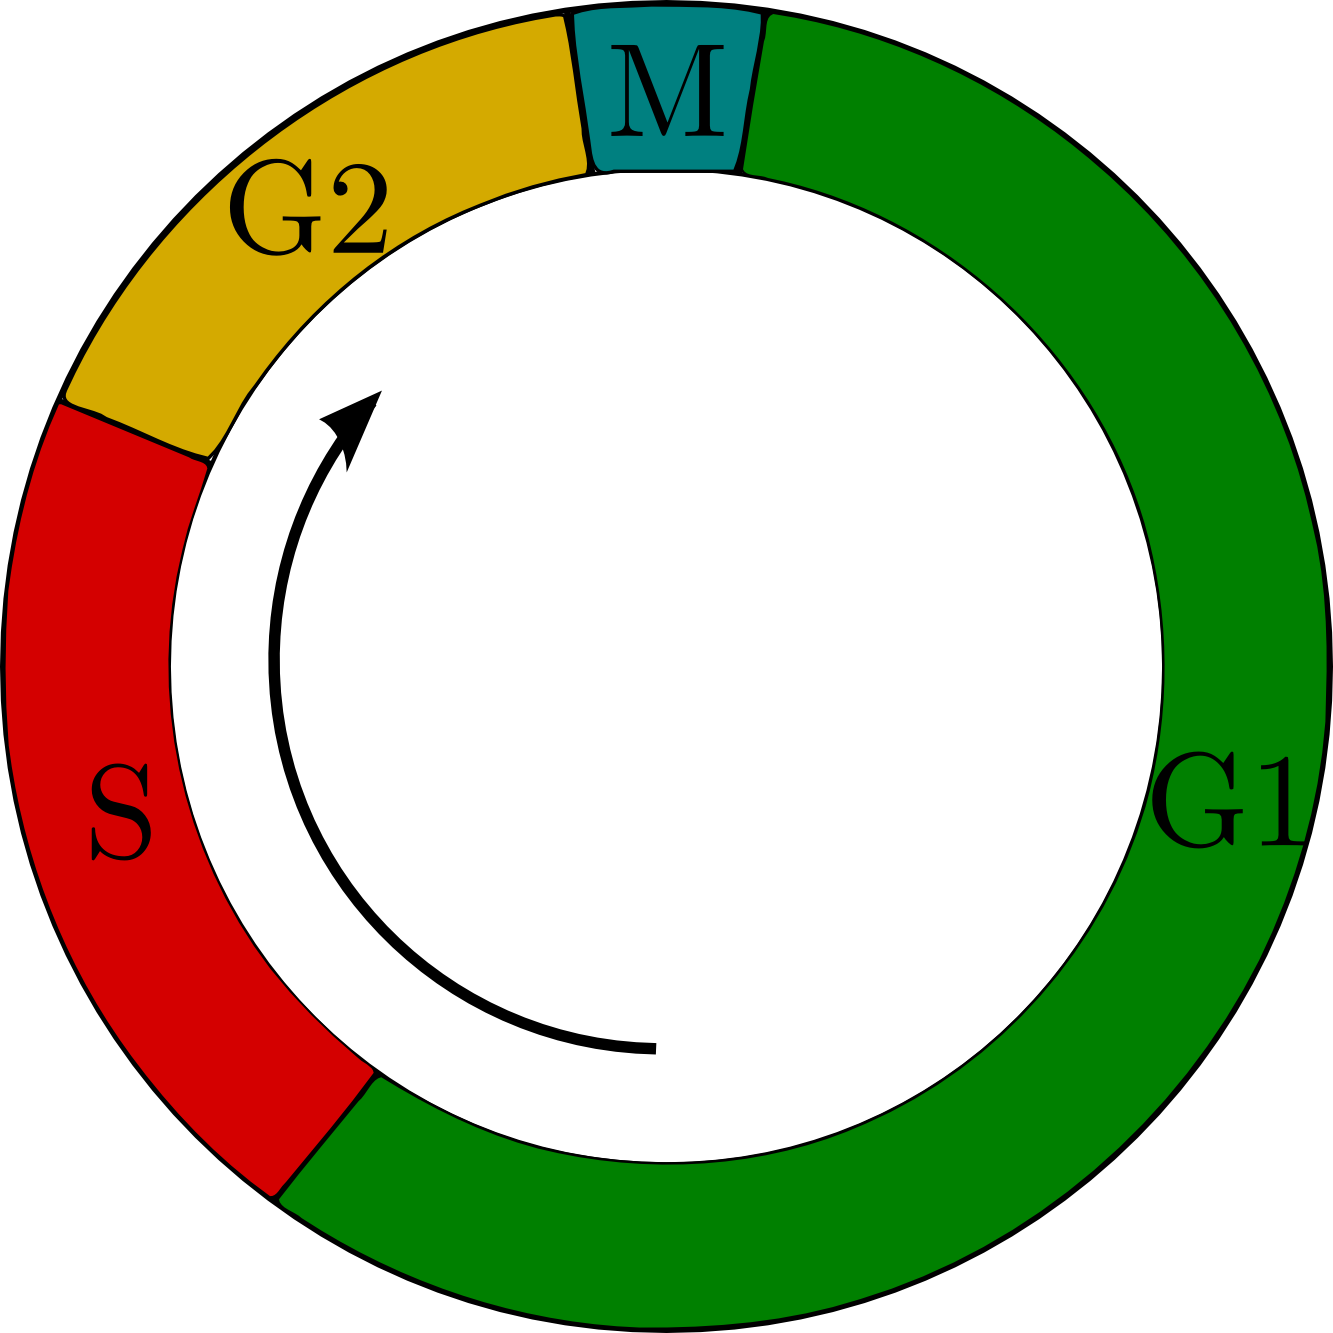
\includegraphics[width=0.95\linewidth]{pngs/cell_cycle.png}
				\caption{Canonical.}
			\end{subfigure}%
			\begin{subfigure}{.33\textwidth}
				\centering
				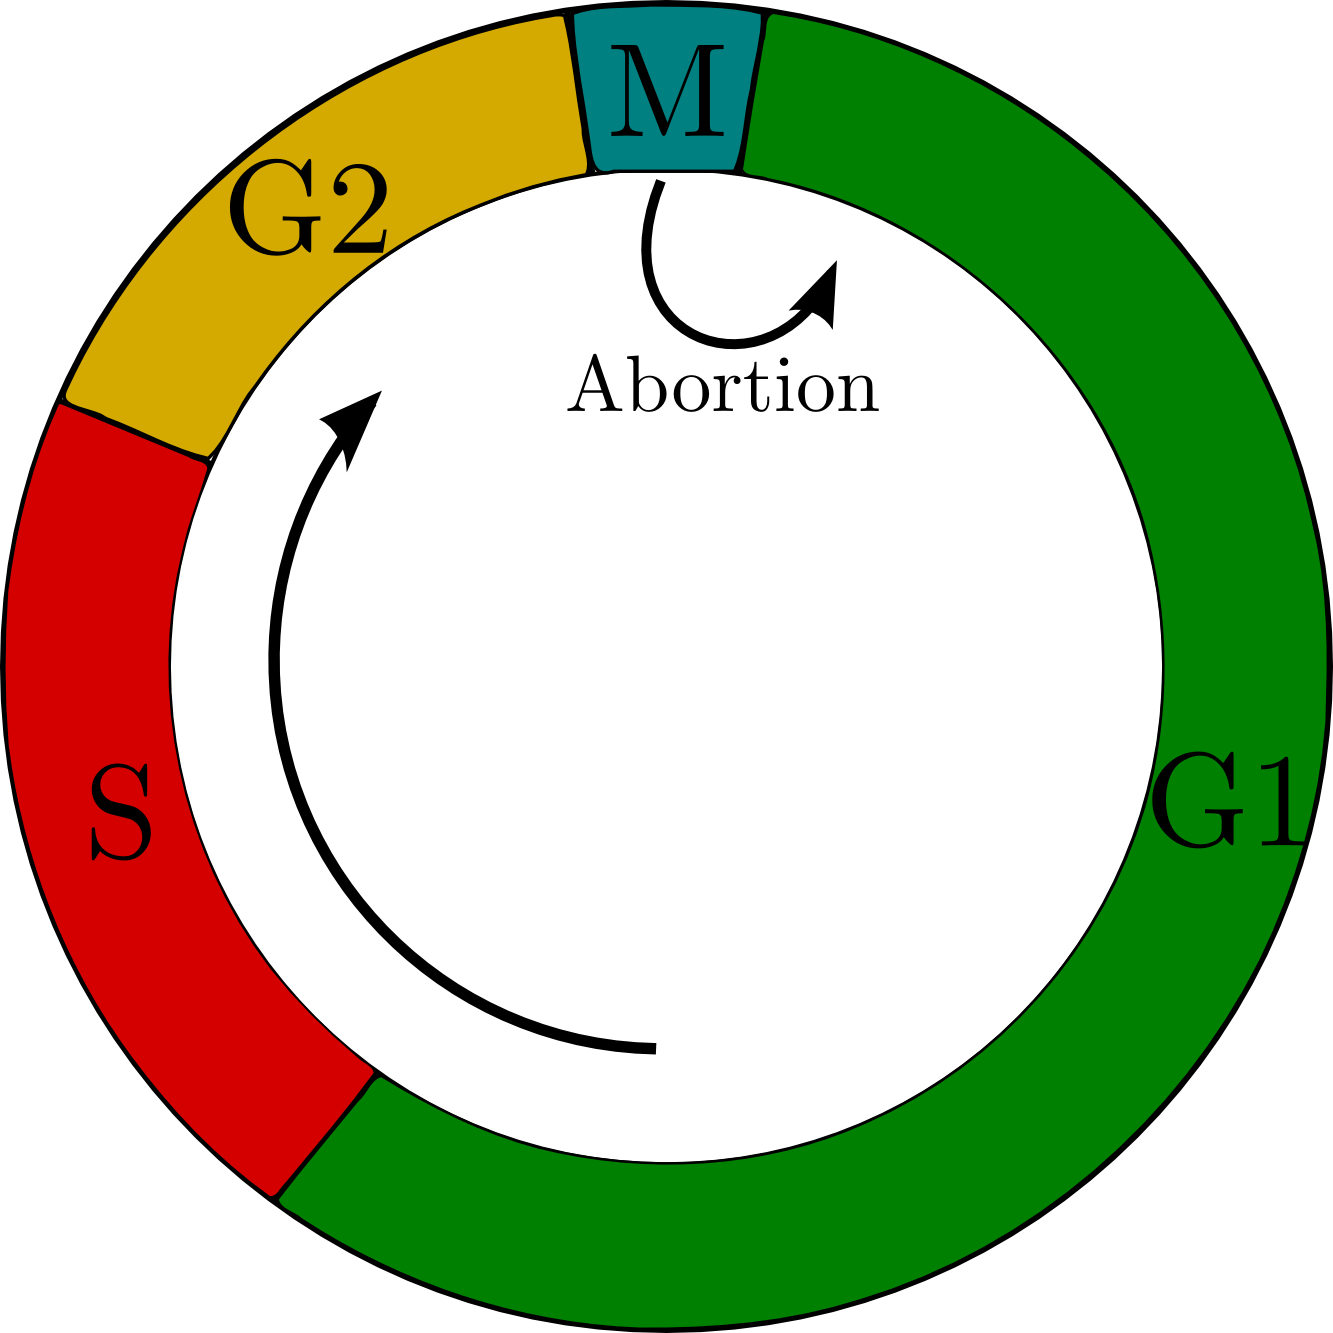
\includegraphics[width=0.95\linewidth]{pngs/cell_cycle_abortive.png}
				\caption{Abortive mitotic phase.}
			\end{subfigure}%
			\begin{subfigure}{.33\textwidth}
				\centering
				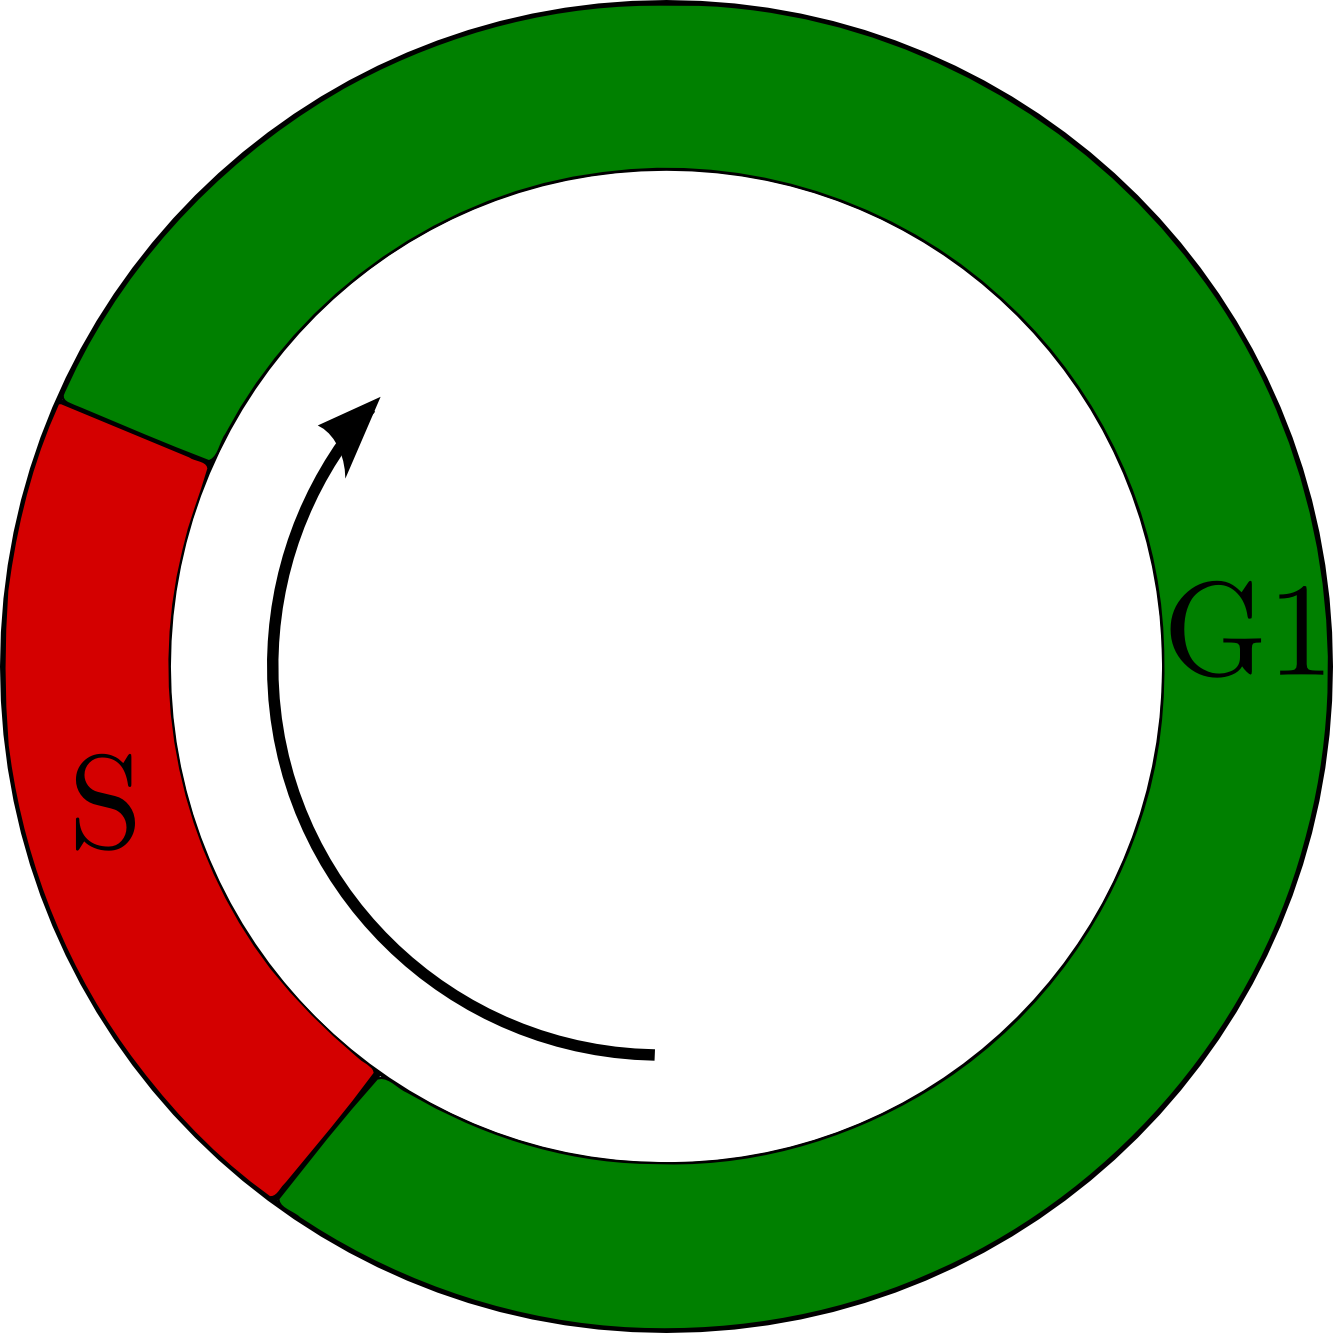
\includegraphics[width=0.95\linewidth]{pngs/endocycle.png}
				\caption{Endoreplicative and Endocycle.}
			\end{subfigure}%
			\caption[Variants of cell cycles employed by eukaryotic organisms]
			{Variants of cell cycles employed by eukaryotic organisms.}
			\label{fig:simple_cell_cycle}
		\end{figure}
		
		
		Most remarkably, the core protein machinery that drives and regulates the canonical mitotic cell cycle performs as well in endocycles.
		%Key signalling factors during development seems to exploit conserved cell cycle pathways to guide a cell into performing endocycling. 
		
			\subsection{An overview of the eukaryotic canonical cell cycle}
			Cell division is a mechanism common to all organisms, being necessary for reproduction and also used for growth and proliferation in multicellular organisms. Regulation of the whole cell cycle and cell division is intricately complex, but is necessary to assure progression into the several phases in a controlled manner. Multicellular eukaryotes in particular, require precise timing and sensing of internal and environmental clues, which is regulated by complex cellular machinery, to achieve correct tissue and organ development.
			
			The canonical cell cycle consists of four major phases: gap phase one (G1) - cell growth and synthesis of required subtracts for DNA synthesis; Synthesis (S) - genome replication; gap phase two (G2) - continued cell growth; mitotic phase (M) - cell division through mitosis. Progression through the cell cycle phases is controlled by a number of checkpoints where genomic and cellular integrity are attested and various internal and external cues are considered, allowing progression, or arresting cell cycle.
			
			Numerous protein classes interact during regulation of the canonical cell cycle, being the complexes formed by Cyclins and Cyclin-dependent kinases (CDK) very prominent. Different CDK-Cyclin complexes are activated throughout the cell cycle, and their specific temporal regulation allows modulation of the activity of specific downstream effectors of cycle progression. While CDKs remain relatively constant through the cycle, the level of the Cyclin subunit is regulated thus restricting the complexes' temporal activity. 
			
				\subsubsection{Regulation of cell cycle progression by Cyclin-CDK complexes}
				In general, the overall activity of CDK-Cyclin complexes increases from G1 to M, being several thresholds of their activity used by the cell to identify the phase it is in. An overview of the major CDK-Cyclin complexes during the phases of the cell cycle can be seen in Figure \ref{fig:cellcycle_complex}.
				
								
				% some CDKs are mitotic, some are...
				The G1 phase is the one with lowest CDK-Cyclin activity. This allows the cell to start replication with the assembly of the replication-specific proteins into a pre-replication complex in DNA sites that will become origins of replication. The assembly of pre-replication complexes during the G1 phase licenses replication and when CDK activity is detected above a threshold, the S phase begins with DNA replication. High CDK activity activates replication but also prevents replication licensing during other phases, for it requires low activity. A unique cell division per cycle is thus assured, for only when CDK activity is abolished at the end of mitosis can the genome be licensed for replication again.
				
				\begin{figure}[here]
					\centering
					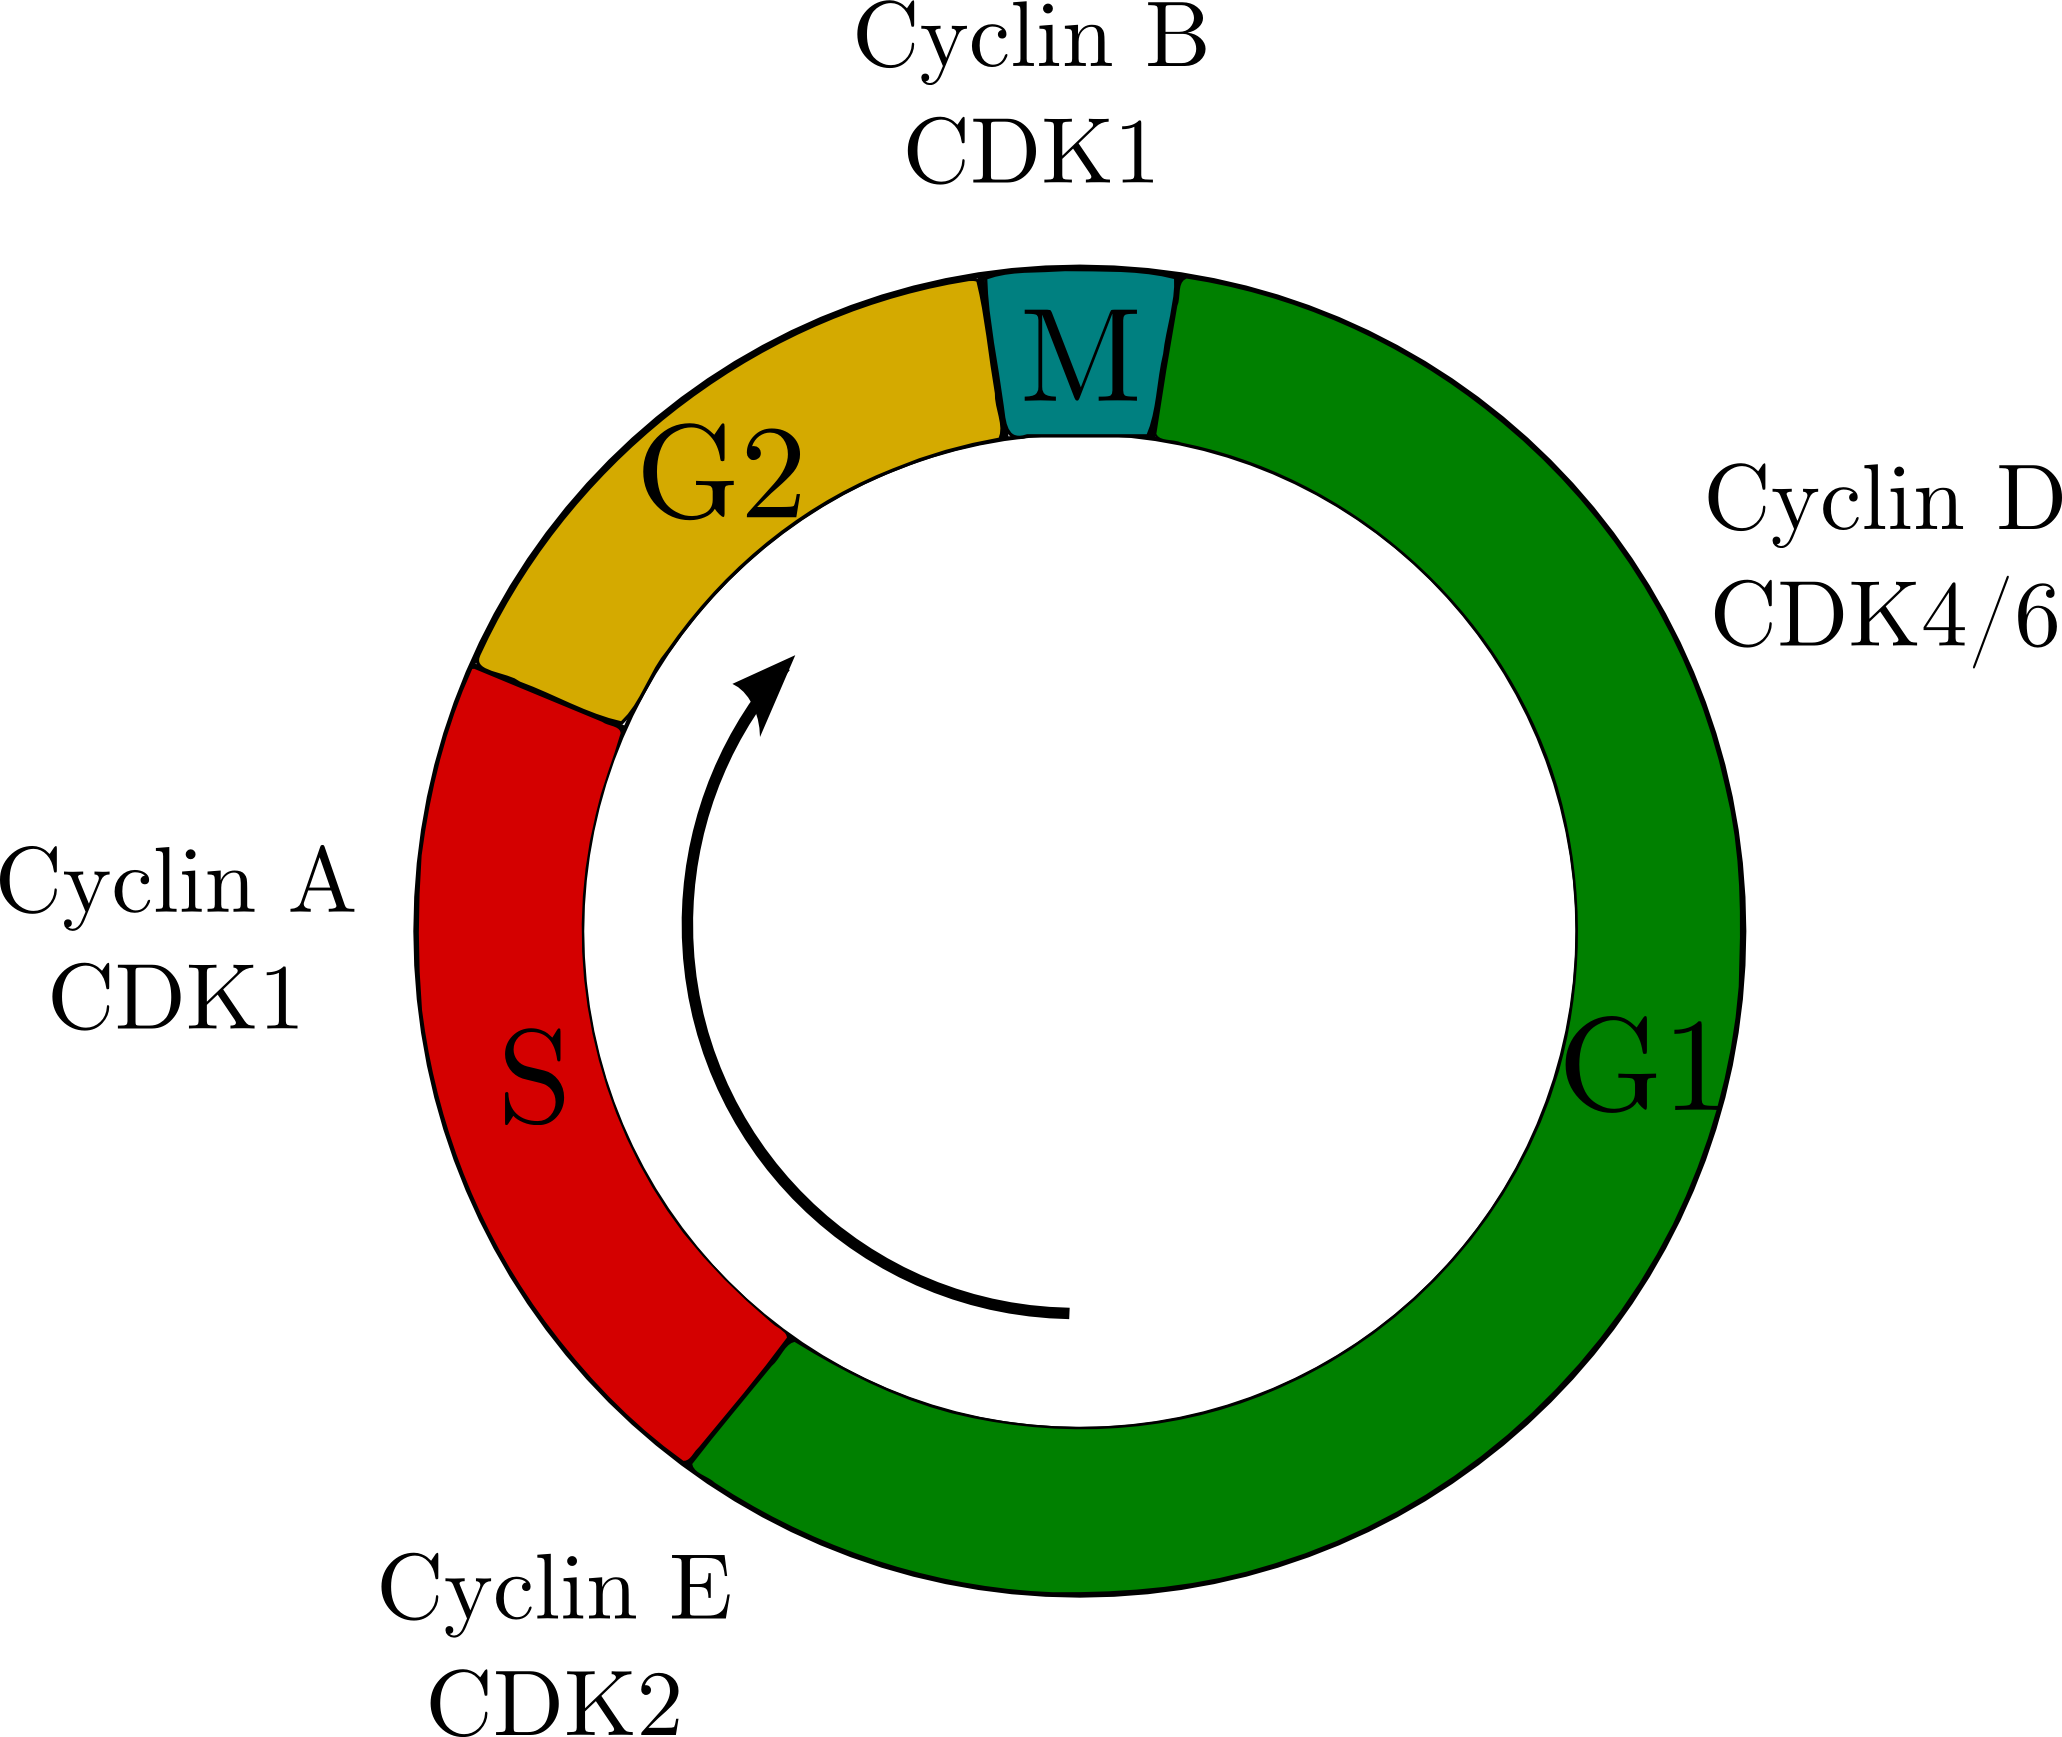
\includegraphics[width=0.5\textwidth]{pngs/cell_cycle_complex.png}
					\caption[Cyclin-CDK complexes during progression of cell cycle phases]
					{Cyclin-CDK complexes during progression of cell cycle phases.}
					\label{fig:cellcycle_complex}
				\end{figure}
								
				In the G1 phase, the D cyclins are expressed in response to external cues such as growth factors. These associate with both CDK 4 and 6 and phosphorilate downstream targets which most importantly include the retinoblastoma protein (pRb). pRb natively binds to a complex formed by a member of the E2F family of transcriptions factors (TF) and DP (also a TF), inhibiting it. When phosphorilated, pRb releases the E2F-DP TF complex and this is free to bind DNA and activate the expression of downstream genes that are responsible for entry into the S phase (Figure \ref{fig:pRb-E2F}).
				
				\begin{figure}[here]
					\centering
					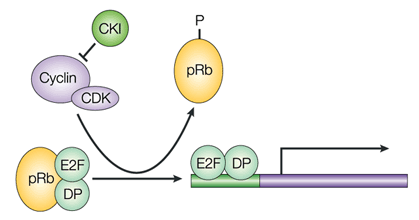
\includegraphics[width=0.5\textwidth]{pngs/CDK-pRb-E2F-DP.png}
					\caption[Cyclin-CDK phosphorilation of pRb and release of the E2F TF during G1 phase of the cell cycle]
					{Cyclin-CDK phosphorilation of pRb and release of the E2F TF during G1 phase of the cell cycle. {\footnotesize Adapted from \cite{Frisch2002}}}
					\label{fig:pRb-E2F}
				\end{figure}
				
				Among the genes regulated by the E2F TF upon S phase entry is Cyclin A. This Cyclin first interacts with CDK2 and this complex is required for successful completion of S phase. Later, Cyclin A complexes with CDK1 having a function in G2/M phases transition.
				
				In the mitotic phase the predominant Cyclin-CDK complex is the Cyclin B-CDK1, which has important functions in phosphorilating cytoskeletal proteins involved in mitosis.
				
				Towards the end of cell division, cyclins are degraded, therefore greatly reducing the overall level of CDK activity. Both A and B cyclins are ubiquitinated by the ubiquitin ligase anaphase-promoting complex/cyclosome (APC/C), which includes the Fzr/Cdh1 subunit. This subunit confers Cyclin A and B specificity, marking them for proteolytic degradation starting at the end of mitosis but continuing through the G1 phase, which helps to ensure unidirectional cell cycle progression.	
				
				Cyclin-CDK activity can also be modulated by Cyclin-dependent kinase inhibitors (CKI). Among the most prominent are p27 which inhibits CDK4 in the pre-S phase Cyclin D-CDK4 complexes - therefore preventing phosphorilation of pRb and E2F release - and CDK 2 in the Cyclin E-CDK2 complex causing the cell to stay in S phase.
				
				Downstream effects of Cyclin-CDK activity involve activation of various cell cycle effectors including cyclins necessary for the subsequent phase, and this is fundamental for all cell cycle events to occur, specially in the beginning of the S phase, and during mitosis, assuring that the latter cannot start without the first and vice-versa, and that once they have started they cannot be reversed. These concepts can be visualized in Figure \ref{fig:canonical_cycle} and will prove useful when considering the implications of an endoreplicative cell cycle - a cycle of G and S phases.
				
				\begin{figure}[here]
					\centering
					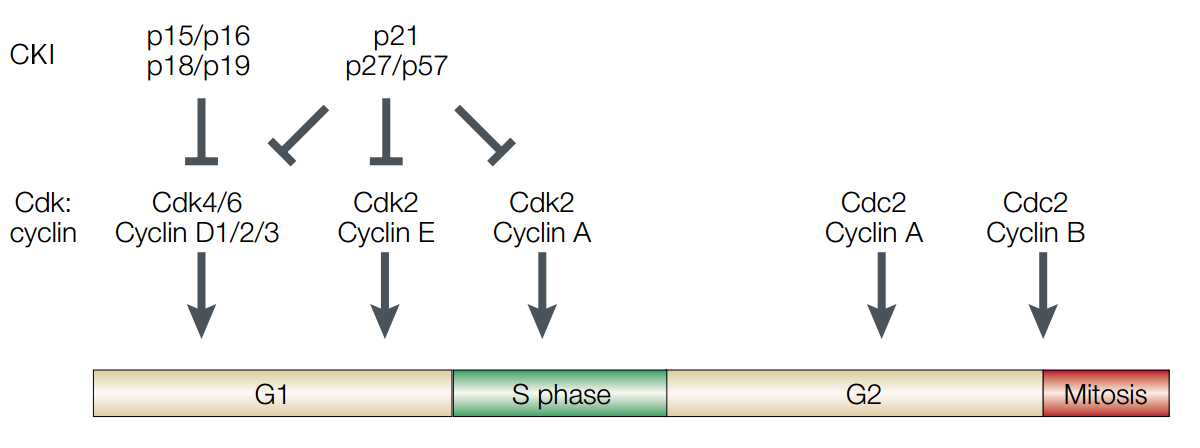
\includegraphics[width=0.9\textwidth]{pngs/canonical_cell_cycle.png}
					\caption[The phases of the canonical eukaryotic cell cycle]
					{The phases of the canonical eukaryotic cell cycle. {\footnotesize Adapted from \cite{Trimarchi2002}}}
					\label{fig:canonical_cycle}
				\end{figure}

			\subsection{Endocycle regulation}
			\label{subsection:endocycles}
			Much less is known about the regulation of alternative modes of cell cycles, endocycling in particular. Compared with the canonical cell cycle regulation, two prominent events must occur for an endocycle to take place:
			
			\begin{enumerate}
				\item abolishment of mitosis and cell division;
				\item alternative regulation of cell cycle effectors to continue to allow genome replication despite that there has been no cell division.
			\end{enumerate}
						
				\subsubsection{Abolishment of mitosis and cell division}
				Bypassing mitosis and cell division in endocycles can be accomplished in several ways. One such way involves the exploitation of the regular regulation mechanism in the canonical cell cycle through modulation of the Cyclin-CDK regulators. 
				The APC/C subunit, Frz/Cdh1 is used in \textit{Drosophila} and \textit{Arabidopsis} as a way to achieve this, and its continued expression is in fact sufficient to induce endoreplication \cite{asd}. Its expression throughout the endocycles is required to continue suppression of pro-mitotic effectors, in particular Cyclin A and B.
				
				Evidence from mammalian cells, specifically placental throphoblas giant cells (TGC) and megakaryocytes in the bone marrow - both employ endocycling - suggest that Cyclin kinase inhibitors (CKI), proteins that act by direct binding to CDKs, also promote endocycling. This happens, with the activation of the p57 protein (a CKI), which inhibits CDK1 and prevents it from actively promoting entry into mitosis.	
				
			 	Blocking cytokinesis is a way to inhibit cell division and thus leads to endoreplication, a mechanism known to be normal in plants, where it has even been used in horticulture to improve crops. RhoA, a GTPase with a key role in regulating cell division is not activated due to the downregulation of two of its activators (GEF-H1 and ECT2) during cytokinesis in magakaryocytes as well, which causes failure of cell division. Endoreplication through an incomplete mitosis, is also known as endomitosis.
			
			\subsubsection{Alternative regulation of cell cycle drivers}
			
				\paragraph{Endoreplication by CDK activity regulation}
			
				The Cyclin E-CDK2 complex is the main driver for S phase entry in the canonical cell cycle, although in the absence of CDK2, CDK1 can act as a substitute in mammalian cells \cite{Ullah2009}. Evidence suggests that modulation of Cyclin E expression during endoreplication in \textit{Drosophila} is crucial and possibly sufficient for its maintenance \cite{Lilly2005}, and megakaryocytes with Cyclin E overexpression show increased ploidy \cite{Eliades2010}, reinforcing the role of Cyclin E complexed with a CDK in endoreplication. The Cyclin E-CDK complex has also been shown to be responsible for the inhibition of the pre-replication complex (RC) protein Orc1 indirectly, by inhibiting the APC/C component Fzr/Cdh1 \cite{Narbonne-Reveau2008}.
			
				All these observations put the Cyclin E-CDK2 complex in the center of regulation of endoreplicative cell cycles: it seems to generally contribute to increased replication, but also inhibits elements necessary for it, indicating that a temporally cyclic regulation of expression is necessary. Cyclin E is present at both transcript and protein level just before and during S phase, but not G, in endoreplicating Drosophila cells \cite{Weng2003} and if expressed continually, endoreplication is suppressed \cite{Weiss}.
			
				\paragraph{E2F factors in CDK activity regulation}
				\label{paragraph:E2Fs}
			
				 The E2F family of TFs is well known to have important functions in the regulation of both the canonical and endoreplicative cell cycles. This family of eight TFs in mammals can be grouped in a set of six canonical and two atypical TFs.
				 Canonical E2Fs dimerize with the DP TF through a XXXXXXXXX domain; E2F3 is duplicated
				 Atypical lack the DP-interaction domain, have two DNA-binding domains which allows homo- and heterodimerization.
							
				Activator E2Fs, after dimerizing with DP are bound by the Retinoblastoma protein (Rb) which prevents its action as TF of binding DNA 
				 (van den Heuvel and Dyson, 2008)
			
				\begin{figure}[here]
					\centering
					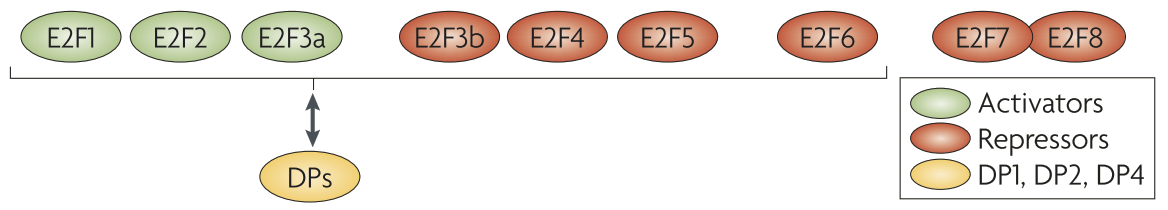
\includegraphics[width=0.9\textwidth]{pngs/E2F_family.png}
					\caption[The E2F family of transcription factors in mammals]
					{The E2F family of transcription factors in mammals. {\footnotesize Adapted from \cite{VandenHeuvel2008}}}
					\label{fig:E2F_family}
				\end{figure}
				
				The most prominent regulator of Cyclin E in the canonical cell cycle is the transcription factor E2F1. It is a potent regulator of S phase entry and DNA synthesis.
				In \textit{Drosophila} endocycles, E2F1 is subject to regulation by the action of CRL4/Cdt2, an ubiquitin ligase that is activated upon DNA replication and thus itself a consequence of the E2F1 activity - a negative feedback mechanism \cite{Zielke2011}\cite{Havens2011}\cite{Shibutani2008}.  There is therefore an oscillation of E2F1 during endocycles that both promotes and is also the consequence of the oscillation of other key players in cell cycle regulation: 
				APC/C activity as a xXXXXXXXX is negatively regulated by Cyclin E-CDK2
				Cdt1 (essential replication licensing protein Cdt1 (Dup - droso))
				Gemini (inhibitor of Cdt1 - inhibited by APC)
				
				\begin{figure}[here]
					\centering
					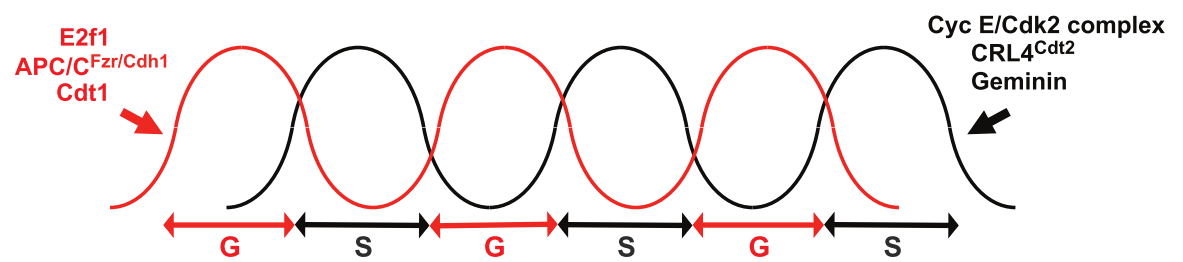
\includegraphics[width=0.9\textwidth]{pngs/oscilation.png}
					\caption[Oscillation of opposing networks of cell cycle genes during endocycles]
					{Oscillation of opposing networks of cell cycle genes during endocycles. {\footnotesize Adapted from \cite{Fox2013}}}
					\label{fig:oscillation}
				\end{figure}
				
				
				This is mechanism of regulation ensures DNA is replicated only once per S phase, and is consistent with the observation that E2F1 activity is necessary for 
				consistent 
			

			Nonetheless, these results emphasize that negative-feedback regulation is a common and important feature of molecular oscillators that control cell cycle progression (Ferrell et al., 2011). A central CDK oscillator provides a mechanism through which other important aspects of endoreplication can be controlled (Fig. 2). 
			For example, the oscillation of APC/C activity in Drosophila salivary glands probably results directly from the oscillation of Cyclin E/Cdk2 complex activity, which inhibits the APC/C (Narbonne-Reveau et al., 2008). Key targets of the APC/C during endoreplication progression are the mitotic cyclins and the protein Geminin, which is an inhibitor of the essential replication licensing protein Cdt1 (Dup – FlyBase).
			Indeed, the combination of mitotic Cdk1 inhibition and Geminin proteolysis can trigger endoreplication in human cells (Hochegger et al., 2007). By contrast, in Arabidopsis, little or no APC/C activity is required for endoreplication progression (as opposed to endoreplication entry, as described above), perhaps because there is no Geminin protein (Roodbarkelari et al., 2010). In Drosophila salivary glands, Geminin is absent during G phase, when replication licensing occurs, and present during S phase to prevent DNA licensing (Zielke et al., 2008).
			 In this way, the endoreplication S phase is similar to the S phase of a cell division cycle and distinct from the phenomenon of re-replication, in which specific segments of DNA are replicated more than once in a single S phase. In contrast to endoreplication, re-replication is an aberrant situation that causes genomic instability and is observed in some cancer cells (see Box 2).
			 In summary, the central endoreplication oscillator entrains many molecular activities to ensure the cycling of CDK activity and, thus, the cycling of replication licensing. It is important to keep in mind that the mechanism by which cyclic CDK activity is achieved may differ among species or even among different cell types within the same organism. For example, Drosophila nurse cells probably rely more on CKI activity than on E2F activity for CDK control during endoreplication (Hong et al., 2007). Nevertheless, the network of interactions controlling cyclic S phase CDK activity constitutes the central principle of endoreplication that we propose is universally applicable.

			Negative-feedback regulation of E2F activity is also important for endoreplication in hepatocytes (Chen et al., 2012; Pandit et al., 2012), but here it appears to control the transition from cell division to endoreplication, and it is not yet known whether E2F functions as part of a mammalian endoreplication oscillator.
			
			
			In another perspective, E2F7 is known to repress a network of cell cycle genes to control S-phase progression.\cite{Westendorp2012}
			\cite{Moon2008}
			\cite{Meserve2012}
			\cite{Chen2012}

	\clearpage
	\section{Histone modifications in cell cycle regulation}
	In the post-genomic era, characterizing the genetic repertoire of a model species is solely the first step to understanding of its Biology from a molecular point of view. Gene regulation is currently the limelight of studies in Biology and Biomedicine and the characterization of gene expression and the mechanisms of its regulation pre- and post-transcription and translation is the current forefront of research. An important contribution to gene regulation comes from epigenetics. Long-non coding RNAs (lncRNAs), histone variants, histone modifications and modification of DNA bases (prominently methylation) are four great classes of mechanisms by which gene expression is altered epigenetically. 
		
	The fundamental structural unit of chromatin is the nucleosome - a structure formed by histone proteins with DNA wrapped around them. A core octamer of histones comprised of two copies of H2A, H2B, H3 and H4 histones each, forms the canonical nucleosome structure to which 147 base pairs of DNA are wrapped around twice. This basic structure repeats itself throughout the genome and provides the basis for higher-order structure in chromatin. The disposition of the histone proteins creates a disc-shaped structure resulting from the left-handed superhelical DNA structure. Since the first structural evidence of the nucleosome, more \textit{in-vivo} nucleosome structures presenting different stoichiometries have been discovered and although in some cases their functional implications have yet to be shown, they have changed the way we look at nucleosomes - it can no longer be viewed as a static identity.

	Genes of histone proteins involved in the formation of the canonical nucleossome have several specific conserved features. They lack introns and are organized in clusters. Due to the occurrence of a major celluclar event requiring a high number of histone proteins - replication in S phase - histone genes are known to be replication dependent (RD). Their expression is coupled with the cellular event of replication by the use of a conserved stem-loop (SL) in the 3’UTR of the mRNAs, which promotes translation in this phase. Genes of variant histone proteins are often transcribed from orphan genes (not in clusters), can contain introns and lack the SL motif that couples translation to replication. Although considerable structural divergence exists, in most cases histone variants (also called replication-independent (RI) histones) are still fairy conserved due to being subject to the structural constraints promoted by the assembly into nucleossomes.
			
	Post-translational modifications of histone proteins were discovered in the mid-1960s and are long known to have a functional role. Due to the fact that most post-translational modifications of histones were found on the protruding histone tails, initial theories suggested they affected the interactions between DNA and histone tails electrostatically. This less stringent DNA-histone link would loosen chromatin structure and make attachment and detachment possible, explaining changes in accessibility of DNA sequence to regulatory proteins and differential position of nucleosomes along the DNA sequence. Later, with better knowledge of the diversity of post-translational modifications of histones and the discovery of more functions associated with them, post-translational modifications of histones are now thought to function as epitopes for regulatory proteins to act on, marking discrete parts of the histone-bound DNA for a specific function. At the same time, discovery of post-translational modifications of histones nearer to the histone core still supported the idea that they also contribute to alter DNA-histone and histone-histone interactions.
	 
	Some post-translational modifications of histones are known to be correlated with gene silencing, others with gene activation, and some correlate with presence or activity of regulatory elements, transcriptional units or replication origins, but although many have been identified and associated with these functions, the exact mechanism but which they achieve this is not entirely known. Common post-translational modifications in histone proteins are methylation, acetylation or ubiquitination of lysines, serine phosphorylation or arginine methylation, but others exist as well  \cite{Strahl2000a} \cite{Kouzarides2007} \cite{Bannister2011}.
	 
	This array of chemical varieties in histones is therefore heavily loaded with information that has been shown to condition gene expression and contribute to triggering of major cellular events (\textit{e.g.} cell division). This information is stably maintained and passed to daughter cells upon cell division which is important for the maintenance of regulatory status along cell division and differentiation. These processes are therefore considered epigenetic because they influence gene expression and are inheritable by daughter cells.
		
	The cell cycle is currently one of the most studied biological processes, due to its significance in growth and development, but increasingly due to its deregulation in many human disorders. Studies using a diverse set of model organisms have greatly expanded knowledge of cell cycle regulation and have contributed to a uniform view of how the basic cell cycle machinery is regulated  \cite{Raynaud2014a}.
	
	Although studied for long, only recently have histone modifications been shown to contribute to it. This chapter of the review highlights the function of some post-translational histone modifications in cell cycle regulation.
		
		\subsection{The role of H2Bub in DNA replication}
		Monoubiquitylation of histone H2B on lysine 123 (H2Bub1) is known to be an important histone modification during transcription. H2Bub1 is promoted by the Bre1 ubiquitin ligase and this happens mainly in coding regions, particularly the ones that are being expressed. It is also a highly dynamic histone modification, with cycles of ubiquitylation and deubiquitylation naturaly occuring during the transcritpional process. I has been shown that this oscilation is required for proper transcriptional elongation through the control of the RNA Polymerase II (Pol II) and inhibition of recruitment of the CTK1 kinase, which has a function in later phases of transcription. H2Bub1 also controls the methylation state of both lysine 4 and 79 residues on histone H3 - two other important modifications in the transcriptional and replicative process \cite{Kouzarides2007}.
		
		The mechanistical similarities between transcription and replication suggest that H2Bub1 may have a role in replication as well. In both processes, nucleossomes must be displaced ahead of the replication fork and assembled again after (in replication in more strands than in the original template).
		
		In recent studies performed in the buddying yeast  \cite{Trujillo2012}, H2Bub1 has been shown to be enriched at replication origins, while the writer of this modification, Bre1, is also present. H2Bub1 continued to be present after replication, during G2 and M phases, suggesting that it is maintained on daughter strands of chromatin and after origins are fired for replication start.
		
		Hydroxyurea, a inhibitor of a ribonucleotide reductase enzyme required for deoxyribonucleotides production, has the effect of causing S phase arrest due to nucleotide depletion. When G1 arrested synchronized cells were released into hydroxyurea, Bre1 and H2Bub1 were detected at regions away from replication origins, posing the hypothesis that Bre1 could be travelling with the replissome as happens in transcription due to Pol II complex association \cite{Trujillo2012}.
		
		Using a mutant strain for H2BK123, it was possible to detect that H2Bub1 was shown to be not required for the initiation of DNA synthesis as mutant cells initiated DNA replication. Nevertheless, when accessed for their capability to complete replication in the same time as wild-type cells, H2BK123 mutants were slower, as accessed by the levels of H3K56ac and the G2/M marker Clb2. This confirmed the involvment of H2Bub1 in normal cell cycle progression, particularly in the elongation of DNA replication in S phase \cite{Trujillo2012}.
		
		Dissecting the reason of the inefficiency of H2BK123 mutant cells in replication elogation, it was shown that in these cell only a fraction of the factors required for replication elongation (Pol $\alpha$, Pol $\epsilon$ Mcm4, Cdc45 Psf2) did not accumulate significantly at positions downstream of replication origins when compared with wild-type cells. Additionaly, reduced intermediate single-stranded DNA was detected in mutants. Toghether this reveals the important role of H2Bub1 in the progression of replication forks, possibly through the interaction with other effectors necessary for replication elongation \cite{Trujillo2012}.
		
		In these mutant cells, it was also noted that global histone H3 levels were reduced in replication origins after replication compared with wild-type cells, pointing to either a defect in nucleossome assembly on newly synthesised strands or reduced stabilization of assembled nucleossomes \cite{Trujillo2012}.
		
		Spt16, a subunit of the FACT complex that is responsible for nucleossome displacement ahead of the transcription fork is known to interact with H2Bub1 to restore nucleossome ocupancy during elongation of transcription. In replication the same was also detected, with Spt16 present at replication origins and more distal positions with the replication fork advancement. However, in H2BK123 mutant cells, Spt16 was significantly reduced in distal replicating positions, suggesting that H2Bub1 stabilizes Spt15 on replicating chromatin \cite{Trujillo2012}.
		
		Taken together, evidence collected in this study \cite{Trujillo2012} showed an unprecedented role for a histone modification in replication. Ubiquitylation of H2BK123 is present in origins of replication, promotes efficient replication elongation and the stability of the replisome as well as nucleosome assembly or stability.
		
		\subsection{Dot1 and H3K79 methylation in the cell cycle}
	
		All known histone lysine methyltransferases contain a SET domain, with the exception of Dot1, which has a conserved catalytic core more similar to arginine methyltransferases. Dot1 is conserved from trypanosomes to humans and catalyses mono-, di- and trimethylation of histone H3K79, a residue located in the nucleosome core \cite{Kouzarides2007}. Until now, no protein has been identified that unambigously binds a specific methylated state of H3K79 or that can remove any methyl group from it \cite{Frederiks2008}.
		
		It has been shown that Dot1's mode of action is distributive \textit{in vivo} and not processive as all SET domain-containing methyltransferases \cite{Frederiks2008}. This means Dot1 acts in a ‘methylate-and-run’ fashion rather than using a multistep processive approach - this makes it the first known distributive protein lysine methyltransferase. This also implies that the initial methylation states of H3K79 are obligatory intermediates in the synthesis of higher methylation states by Dot1.
		
		The earliest known function of H3K79 methylation was in euchromatin, where it restricts Sir-mediated silencing of chromatin to regions of silent chromatin \cite{Frederiks2008}. In this function there is no correlation between the level of any of the specific methylation states and the degree of silencing, but the sum of all methylation states is indeed correlated, which implies that the different methylation states are likely to have redundant functions.
		
		It is also known that di- and trimethylation of H3K79 in yeast requires ubiquitination of histone H2B on Lys123 (H2Bub1) which is deposited by the Bre1 ubiquitin ligase. Bre1 does not specifically regulate H3K79 methylation but instead enhances its overall catalysis \cite{Kouzarides2007} \cite{Frederiks2008}. This has been proposed to be due to the possibility that the ubiquitin moiety directly affects the active site of Dot1 or that H2Bub1 affects the \textit{in vivo} chromatin substrate such that H3K79 on the nucleosome core becomes more accessible for interaction with Dot1 \cite{Frederiks2008}. The second option seems more supported due to the fact that \textit{in vitro}, H2BK123ub1 is not required for multiple methylation of H3K79 by Dot1.
		
		Dot1's distributive mode of action has prompted the mathematical modelling of H3K79 methylation states in yeast, using quantitative proteomics data, growth rates and estimates of nuclear Dot1 and histone abundance \textit{in vivo} \cite{DeVos2011}. This model predicts that increased states of H3K79 methylation accumulate with time until a H3K79me3-rich steady state is reached. Another important prediction is that each subsequent methylation reaction is slower than the one before - in agreement with a non-processive mechanism of methylation \cite{DeVos2011}.
			
		Since all states of H3K79 methylation accumulate during a cell's life cycle, one prediction of the model is that cell-cycle length can affect the average pattern of methylation throughout the cell cycle phases. This was confirmed experimentally with the observation that in slowly growing or arrested cells, H3K79 methylation is indeed higher, probably due to the fact that Dot1 has more time to introduce methyl groups. Over all cell cycle stages, it was noted a temporary drop in methylation during S phase, when new, unmodified histones are deposited on chromatin \cite{DeVos2011}. The level of H3K79me0 was highest in the S phase but progressive accumulation of methyl groups until a new S phase. This would implicate that H3K79 methylation is at least not fully maintained on new histones during replication. Nevertheless, only when the cell cycle time was doubled, a steady state of high H3K79me3 was reached, indicating that in a normal yeast cell cycle a steady state is not reached and histone renewal might play a role on the balance of H3K79 methylation \cite{DeVos2011}.
		
		The model thus accurately predicted the dynamics of H3K79 methylation through cell cycle and highlighted the importance of the residence time of histones in chromatin.	It was shown experimentally that the level of H3K79 methylation correlates with the age of the histones, regardless of the cell's age and that nucleossomes binding genes known for high histone turnover had significantly less H3K79 methylation. These observations confirm the temporal dependency between H3K79 methylation and the age of histones. The same dependency was not detected in H3K4 methylation, suggesting that the presence of a demethylase can counteract the accumulation of methylation on ageing histones \cite{DeVos2011}.
		
		This temporal dependence of H3K79 methylation has additional implications: epigenetic inheritance of H3K79 methylation states is hindered by the fact that at least one of the daughter cells will not receive the same information as the parent cell. This is incompatible with the current model of histone modification as marks of epigenetic memory. However it shouldn't be excluded that not the information of single nucleossomes, but the global state of H3K79 methylation over larger chromatin domains might bare epigenetic function.
		
		Figure \ref{fig:dot1_k79}.
		
		\begin{figure}[here]
			\centering
			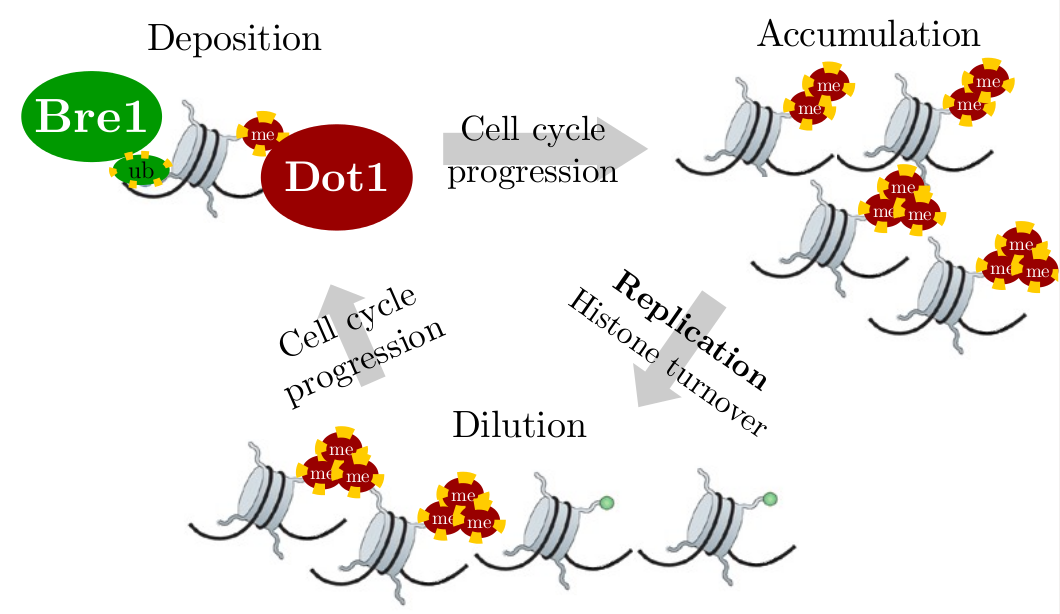
\includegraphics[width=0.9\linewidth]{pngs/dot1_k79.png}
			\caption{Schema of the dynamics of H3K79 methylation during a cell's cycle.}
			\label{fig:dot1_k79}
		\end{figure}
		
		In \textit{Trypanossoma} - a unicellular eukaryotic parasite with considerable divergence of key cell cycle regulators - the view of H3K79 methylation (H3K76 in \textit{Trypanossoma}) as a carrier of epigenetic information is also challenged by the depletion of H3K79 methylation on newly incorporated histones during S phase \cite{Gassen2012}.
		
		In this organism there are two Dot1 homologue proteins of Dot1 (Dot1A and Dot1B) and there seems to be some division of labour between the two regarding the different methylation states of H3K79. Although both enzymes can mono- and dimethylate H3K79, Dot1A seems incapable of trymetylating H3K79, whereas Dot1B does, but it is not clear if both enzymes have the same affinity for the two shared methylation forms and therefore contribute equally \cite{Gassen2012}. Only Dot1A is required for survival.
	
		Depletion of Dot1A decreased H3K79 mono- and di-methylation and generated cells with reduced DNA content, which suggests a role for H3K79 methylation in accurate cell-cycle progression. These cells suffered complete replication inhibition which nevertheless didn't prevented cell division \cite{Gassen2012}.
		
		The inverse disturbance in Dot1A expression (overexpression) resulted in premature H3K79 methylation (during S phase) opposed to generalised increase of methylation levels. Nevertheless, this temporal deregulation caused continuous DNA replication which created cells with increased levels DNA content - the opposite effect of Dot1A depletion. This suggests that not only the global methylation states of H3K79 are implied in accurate cell cycle regulation, but that the timing of addition of this histone modification also plays a role at least in \textit{Trypanossoma} \cite{Gassen2012}.
		
		In human cells, depletion of Dot1, and consequently H3K79 methylation, did not seem to affect replication mechanism itself since the frequency of replication initiation events, replication fork velocity and the proportion of cell cycle phases were not different when compared with normal cells \cite{Fu2013a}. However, an increased fraction of cells exhibiting DNA content greater than 4N and apoptosis was detected.
		
		Although cells were still able to proliferate and replicate DNA in the absence of H3K79 methylation, its absence affected the regulatory processess modulating the timing of DNA replication, for the causes of a higher fraction of cells with higher ploidy than normally were identified as cells skipping mitosis after S phase and re-replicating their DNA without completing cell division \cite{Fu2013a}.
		
		This deregulation of replication timing led to the hypothesis that Dot1 mediated H3K79 methylation marks origins of replication that have started replication, preventing replication initiation a second time before the cell completes division. In the case of cells lacking Dot1, the cause of re-replication might then be new replication from origins or replication that had already been used previously in the same cell cycle. This hypothesis is supported by evidence that H3K79me2 was shown to be associated with functional replication origins, but not with a mutant replication origin that resembled a functional one \cite{Fu2013a}.
		
		These studies highlight the non-canonical use of a histone modification (H3K79 methylation) and show its importance in the regulation of replication, a major cellular event.

	\clearpage
	\section{\textit{Oikopleura dioica}, a marine chordate extensively employing endocycles}
		\textit{Oikopleura dioica} is a marine  chordate organism belonging to the class Appendicularia, which is a member of the Tunicate subphylum along with the classes Thaliacea (salps) and Ascidiacea (sea squirts). Tunicates are the most closely extant group related to the vertebrates (see Figure \ref{fig:tree}) \cite{Delsuc2006}. \textit{Oikopleura} shares some biological traits with most tunicates (\textit{e.g.} filter feeding through a secreted house), but unlike them has some peculiarities which make it a very interesting model for the study of many biological features, such an accelerated development and life cycle, a miniature genome and an extensive use of endocycles through its life. \textit{Oikopleura dioica} owes its name to the fact that it is the only dioeicious appendicularian known, being most other species hermaphrodites.
		
		\begin{figure}[here]
			\centering
			\begin{subfigure}{.5\textwidth}
				\centering
				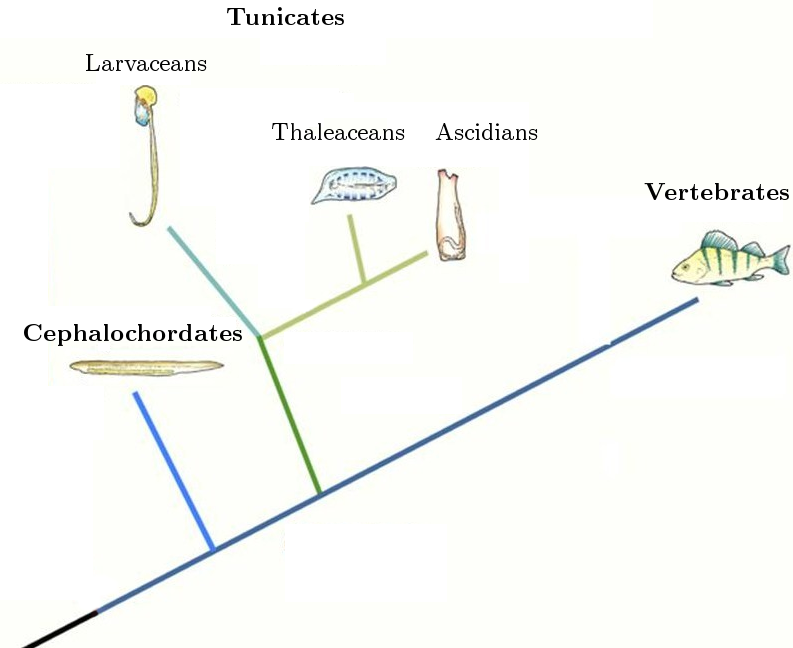
\includegraphics[width=1\linewidth]{pngs/phylogeny.png}
				\caption{Simplified phylogeny of the Tunicate group.}
			\end{subfigure}%
			\begin{subfigure}{.5\textwidth}
				\centering
				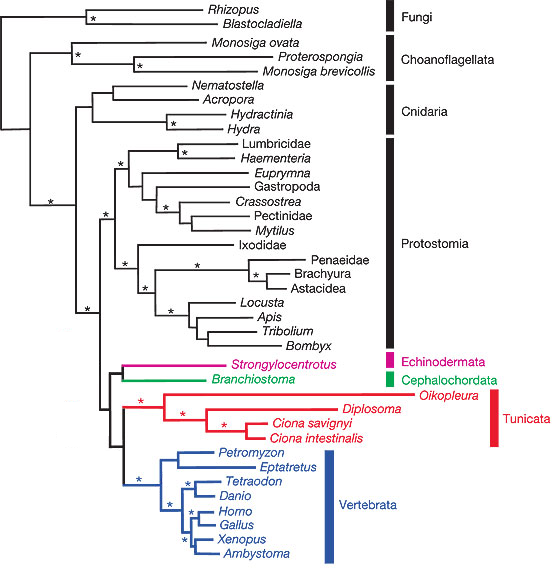
\includegraphics[width=1\linewidth]{pngs/tree.png}
				\caption{Phylogenetic tree including the position of \textit{Oikopleura}.}
			\end{subfigure}
			\caption[Phylogenetic position of the Tunicate group and \textit{Oikopleura}]
			{Phylogenetic position of the Tunicate group and \textit{Oikopleura dioica}.
				{\footnotesize
					Adapted from a figure by Charlotte Konikoff at the University of Washington and \cite{Delsuc2006}.
				}
			}
			\label{fig:tree}
		\end{figure}
		
		\subsection{\textit{Oikopleura}'s life cycle}
		\label{subsection:lifeCycle}
		\textit{Oikopleura} reproduces through external fertilization after the rupture of both female and male gonads or sperm release via the spermiduct \cite{Bouquet2009}. The first cell division remarkably occurs only 35 min after fertilization proceeds with a basically bilateral pattern with minor left–right asymmetries. Gastrulation takes place starting at the 32-cell stage (roughly two hpf at 20ºC) and progresses until all of the vegetal cells have ingressed and are covered by the animal cells. By the 64-cell stage eight cells disposed in two rows of four align themselves along the anterior-posterior axis and are internalized giving rise to the neural tube later. This simple but accelerated early development of \textit{Oikopleura}, gives rise to a conserved chordate body plan with the animal bent ventrally inside the chorion (Tailbud stage) soon hatching and becoming a free-swimming larva \cite{Fujii2008}.
		
		Larval development takes place until fifteen hours after fertilization, where a metamorphosis known as Tailshift occurs: the tails changes orientation towards the ventral side of the animal. At this point, most cells have stopped mitotic division and start performing endocycling, a endoreduplicative cell division strategy which gives rise to multinucleated cells (> 1000 C \cite{Ganot2002})and increases body size by increasing the cell volume rather than cell division (discussed in detail in Section \ref{subsection:endocycles} and \ref{subsection:CellCycleVariants}). \textit{Oikopleura} secretes a extracellular, cellulose-based structure through its epithelium (‘tunics’ or ‘houses’) which uses to filter particles in suspension to feed on and sustain growth. This growth strategy continues throughout most of the remaining juvenile life of \textit{Oikopleura} until the third day of development, where gonad development starts.
		
		Most of \textit{Oikopleura}'s growth until the end of its life at day six is dedicated to gonad maturation, which at its peak reaches a total volume bigger than the somatic part of the whole organism. This is achieved again through the employment of endocycling in the gonad tissues, creating a giant cell of over 2000 C. In the female gonad, a process of nuclei selection occurs, where some nuclei are selected to become oocytes and other nurse nuclei, providing support for the selected nuclei and then degenerating towards the end of maturation. Male gametogenesis is known to start later than the female and is a fast process occuring just before full maturation.
		
		An overview of the different phases of development of \textit{Oikopleura} can be seen in 	Figure \ref{fig:LifeCycle}.
		
		\begin{figure}[here]
			\centering
			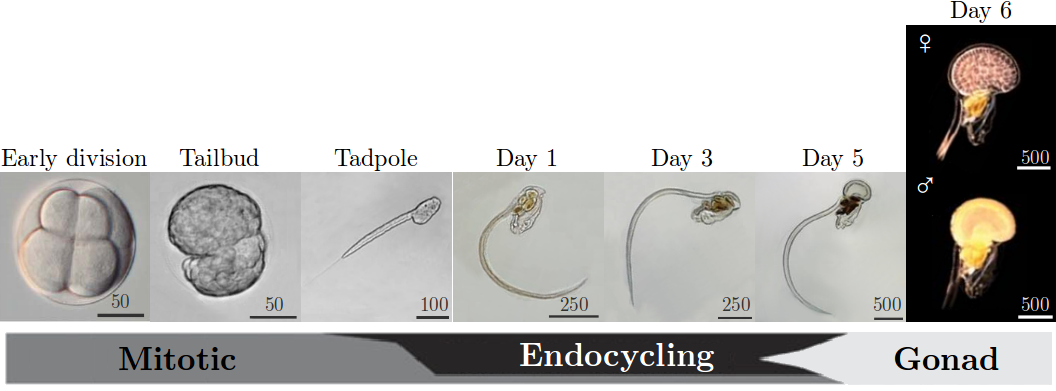
\includegraphics[width=1\textwidth]{pngs/lifeCycle.png}
			\caption[Development of \textit{Oikopleura} and respective predominantly employed modes of cell cycle]
			{Stages of development of \textit{Oikopleura dioica} and respective predominantly employed modes of cell cycle.
				{\footnotesize
					Scale in micrometers. Adapted from \cite{Fujii2008} and \cite{Bouquet2009}.
				}
			}
			\label{fig:LifeCycle}
		\end{figure}
		

		\subsection{The genome of \textit{Oikopleura dioica}}
		A reference sequence of \textit{Oikopleura dioica} genome was made available in 2010 \cite{Denoeud2010a}, revealing a surprisingly plastic architecture and the species fast evolution. In this planctonic animal, the chordate genome architecture seems to have been redesigned to obtain a minimal-sized genome: approximately 70 megabases. This is greatly due to the reduction of intron and intergenic space, although some gene loss was also detected.
		
		The dramatic reduction of intergenic space brings obvious constrains in terms of gene regulation, which is to some degree easily seen by the normal occurrence of genes in Operons (~28\% of the 18000 total), and makes the \textit{Oikopleura} genome one of the most compact of all known chordate genomes. Operons are significantly enriched for genes involved in house-keeping functions, while genes involved in developmental processes are significantly under-represented in Operons \cite{Denoeud2010a}.

		Although the idea of generalised simplicity in regulatory mechanisms could be an hipotesis due to the high density of the genome, insights from two distinct populations of \textit{Oikopleura} seem to contradict this. Highly conserved elements in non-coding regions have been found through genomic alignments of Atlantic and Pacific \textit{Oikopleura dioica} \cite{Denoeud2010a}. Besides those, several other conserved genomic features can be found in the \textit{Oikopleura} genome. 	Long introns are more likely to be descendants of ancestrally conserverd introns than the shorter ones, and genes important for development show twice as much more ancestral introns when compared to all annotated genes. Nevertheless, major changes in the number and syntheny of cis regulatory modules (promoters and enhancers) compared with other Tunicates are likely to have occured due to major loss of gene syntheny and the fast evolutionary rate of \textit{Oikopleura}.
		
		\subsection{Histone variants and modifications of \textit{Oikopleura dioica}}
		In \textit{Oikopleura dioica}, the diversity of histone variants and their use through development has been profiled with a mass spectrometry approach \cite{Moosmann2011}. \textit{Oikopleura} possesses a histone complement of 31 histone variants which can be grouped in distinct sets of developmental expression profiles throughout its life cycle. Most common histone variants are present, although remarkable absences can be seen in the macroH2A and H2AX histone variants. A significant expansion of the histone complement exists in \textit{Oikopleura}, which is even further diversified by the existance of alternative splicing on some variants. Additionally, a remarkable set of 15 male-specific histone variants was discovered \cite{Moosmann2011}.
		
		Histone modifications also occur extensively in \textit{Oikopleura} \cite{Moosmann2011}.	Mass spectrometry identified 40 different post-translational modifications (PTMs) in structurally distinct locations. Histone modifications involved in transcription and marking of cis-regulatory elements such as mono-, di- and tri-methylation of lysine 4 in histone 3 (H3K4me1/2/3), acetylated lysine 27 on histone 3 (H3K27ac), are present. 
		Repressive marks with different modes of action were also found such as the constitutive heterochromatin marker trimethylation of lysine 9 of histone H3 (H3K9me3) and the mark layed by the Polycomb-Repressor Group (PRG) of proteins trimethylation of lysine 27 on histone H3 (H3K27me3). Histone marks related with the control of replication such as all methylation states of lysine 20 in histone H4 (H4K20me), monoubiquitinilation of lysine 123 in histone H2B (H2BK123ub1) and methylation of lysine 79 in histone H3 (H3K79me) , the later two of particular interest in this work.
		
		Regarding the function of histone modifications in the cell cycle, conservation of the function of phosphorilation of serine 10 and 31 in histone 3 (H3S10p and H3S31p) was detected \cite{Schulmeister2007} and \cite{Ganot2008}. These modifications are a marker for the mitotic phase of cell cycle, present in the diplotene/diakinesis where they have been shown to contribute to normal chromosome segregation and transmission during mitosis and meiosis. H3S10p is also a mediator of gene silencing at different stages of the cell cycle. Phosphorylation of serine 28 of H3 (H3S28p) also occurs during mitosis where it is seen as a licensing factor and indicating the state of readiness of chromosomes to undergo separation after metaphase rather than as a driving force in chromosome condensation.
					
		\subsection{The cell cycle modes of \textit{Oikopleura dioica}}
		\label{subsection:CellCycleVariants}
		\textit{Oikopleura dioica} employs an unique combination of different modes of cell cycle through its life cycle (see section \ref{subsection:lifeCycle}). This is unique because most cells switch from rapid mitotic division to endocycles around the event of tail shift. Nevertheless, not much is known about the regulation of the alternative cell cycle modes of endocycling in the somatic and gonadal tissues and even less on how can cells change from one to other.
		
		In a study of the diversity of \textit{Oikopleura}'s Cyclin and Cyclin-dependent kinases (CDK) \cite{Campsteijn2012}, it was shown that the complement of cyclins involved in transcriptional regulation is similar to other high invertebrates, whereas the complement used for cell cycle regulation has significant amplifications, specially in the cyclin D, B and CDK1 families. Remarkably, some families are extended not only by gene duplication by by the existence of alternative splice forms, such as in the Cyclin Db. Many of the Cyclin and CDK proteins are expressed exclusively and distinctively during the later stages of development that follow sex differentiation and gonad maturation, showing an important link between complex biological features and gene regulation.
		
		Amplification of the CDK1 family to five paralogs of this mitotic CDK is somewhat unexpected due to the necessity of suppression of CDK1 activity by the activation of APC/C (Cdh1/Fzr) in \textit{Drosophila} and mammalian endocycles. Due to the extensive use of endocycles, amplification of the families of CDK regulating the G1/S phases (CDK 2 or 6) would have been more anticipated. Also very suspicious is the expansion of the Cyclin D family, leading to the hipotesis that regulation through CyclinD-CDK1 complexes specially during the late developmental stages could provide the regulatory refinement needed to control such a complex system as the female coenocyst.
		
		Nevertheless, the \textit{Oikopleura} somatic endocycle resembled features known to be present in endocycles in other systems such as the downregulation of cyclins B and A as in the \textit{Drosophila} and vertebrate mammalian throphoblast giant cells endocycles.
		
		Regarding other key cell cycle regulators, \textit{Oikopleura} possesses a fairly conserved set of proteins involved in regulation of cell cycle both upstream and downstream of the Cyclin-CDK effectors. Of particular notice, the E2F family of transcription factors is reduced when compared with vertebrates or other invertebrates such as \textit{Drosophila}. In \textit{Oikopleura} there is only a canonical activator (E2F1) and a atypical repressor (E2F7) (see more about the E2F family of transcription factors in section \ref{paragraph:E2Fs}).
		
		\subsection{Growth arrest}
		\label{subsection:Growth_arrest}
		Developmental processes such as reproduction can be regulated by environmental conditions. In an array of organisms, the trigger for maturation of reproductive can be delayed or paused in unfavorable conditions. Two particular examples can be seen in the nematode \textit{Caenorhabditis elegans} and the fruitfly \textit{Drosophila melanogaster}, where the loss of germline stem cells (GSCs) has the consequence of extending the lifespan of the organism by evolutionarily conserved signaling pathways \cite{Kenyon2010}. The reverse situation has also been detected, when under nutritional deprivation, these models sacrifice a portion of GSCs that have already entered meiosis, maintaining only a small pool of active GSCs \cite{Subramaniam2014}.

		In \textit{Oikopleura dioica}, nutritional stress caused by cultivation in high density has shown to induce a condition of growth arrest (GA) where somatic endocycling ceases 	and the lifespan of the animal is expanded at least three-fold. In contrast with the previously mentioned models, \textit{Oikopleura} only enters GA condition before the start of meiosis. If nutritional deprivation is encountered after, GA is not induced and maturation occcurs at the same time, but animals have a reduced offspring \cite{Subramaniam2014}.
		
		The GA condition therefore represents a state of suppression of proliferation in the somatic endocycles and could be exploited for experimental purposes in understanding endocycle regulation.
	
	\clearpage
	\section{Project Goals}
		The general aim of this Master thesis was to study the regulation of the different \textit{Oikopleura} cell cycle modes and the transition between them. Although much is known about the canonical eukaryotic cell cycle and to some extent about endocycles, knowledge on the mechanism cells use to transition between different modes of cell cycles is still quite reduced.	 To broaden knowledge on this topic, this thesis studies specifically the role of the E2F transcription factors in these cycles by identifying putatively regulated genes during developmental stages with predominant use of either the canonical mitotic cycle or endocycling.
		
		\begin{figure}[here]
			\centering
			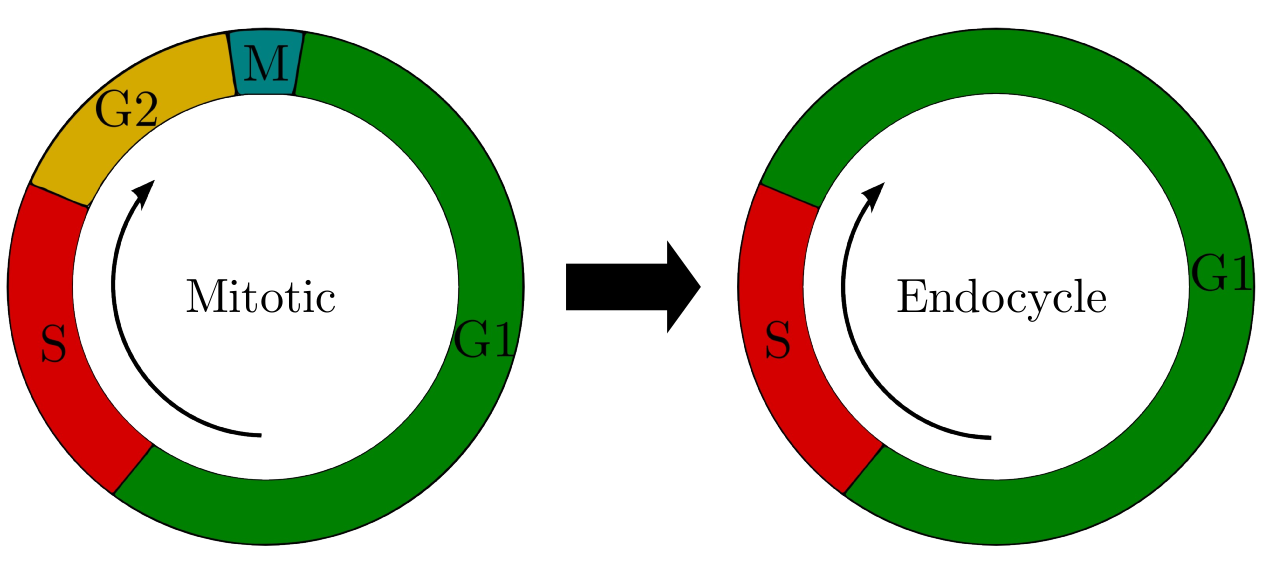
\includegraphics[width=0.7\textwidth]{pngs/change_cell-cycle.png}
			\caption{Goal: to gain understanding of the mechanisms behind the change of cell cycle modes in \textit{Oikopleura}.}
			\label{fig:goal_cycles}
		\end{figure}
		
		To that end, ChIP-seq on the E2F1 and E2F7 transcription factors was performed in the Tailbud (mitotic), Day 2 (somatic endocycle), Day 6 female (gonadal endocycle) and Day 6 male (mitotic) developmental stages. ChIP-chip data on the last two stages had been previously acquired and it is here explored to highlight the differences on these two modes of cell cycle.
		
		A much less explored component of regulation of cell cycles is the influence histone modifications have. Methylation of lysine 79 on histone H3 (H3K79me) has been proposed to act as a timer for a cell's age due to the distributive mechanism of action of its histone methyltransferase - Dot1 - and the absence of a demethylase, which causes the accumulation of this histone mark along the cell's life	.
		
		Another major goal of the project was to gain insights on the regulation of the different cell cycle modes by performing functional studies on the Dot1 histone methyltransferase, and consequently on the function of H3K79me during different modes of cell cycle in \textit{Oikopleura dioica}. This was accomplished by the use of a chemical inhibitor of Dot1 in the Tailbud stage (mitotic) and the Day 5 (endocycle) and characterization of the phenotypic effects of inhibition from a developmental and cellular point of view.
		
\clearpage

%=========================================================================%
\chapter{Materials and Methods}
%=========================================================================%
	\section{Materials}
		\subsection{Antibodies}
			\begin{table}[H]
       		\caption{\bf{Antibodies used for ChIP, immunofluorescence and western blot}}
        		\begin{center}
            		\begin{tabular}{p{2cm} | p{8cm} | p{3cm} | p{3cm}}
	                	\textbf{Antibody} & \textbf{Description} & \textbf{Supplier} & \textbf{Purpose}\\
    		            \hline
        		        ab46540 & Rabbit Control IgG - ChIP Grade & Abcam & ChIP\\
            		    ab & RNA Polymerase II CTD & Abcam & ChIP\\
            		     & E2F1 & & ChIP\\
						 & E2F7 & & ChIP\\
            		    ab10543 & Anti-Histone H3 (phospho S28) [HTA28] & Abcam & Immunostaining\\
            		    39143  & Anti-Histone H3 K79me2 Rabbit & Active Motif & Immunostaining and Western blot\\
            		    05-1312  &  Anti-Ubiquityl-Histone H2B Mouse & Milipore & Immunostaining\\
            		    \hline
            		    A-21206 & Anti-Rabbit IgG secondary antibody conjugated with Alexa 488 fluorochrome &  Molecular Probes & Immunostaining\\
               		    & Anti-Mouse IgG secondary antibody conjugated with Alexa 488  fluorochrome &  & Immunostaining\\
            		    & Anti-Rat IgG secondary antibody conjugated with Alexa 568 fluorochrome & & Immunostaining\\
            		    & Anti-Rabbit IgG secondary antibody conjugated with horseradish peroxidase &  & Western blot\\
	            	\end{tabular}
    		    \end{center}
		    \end{table}
		  
		\subsection{Chemicals and reagents}
		
			\begin{table}[H]
       		\caption{\bf{Chemicals and reagents used in various protocols}}
        		\begin{center}
            		\begin{tabular}{c|c|c}
	               		Supplier & Chemical & Purpose\\
    		            \hline
    		            Thermo Scientific & 16\% Formaldehyde Ampoules, Methanol-free & ChIP\\
    		            Tocris Bioscience & SGC0946 & H3K79me studies\\
	            	\end{tabular}
    		    \end{center}
		    \end{table}
    
	    \subsection{Consumables}
	    \label{subsection:consumables}
			\begin{table}[H]
       			\caption{\bf{Consumables with particular relevance in certain protocols}}
        		\begin{center}
            		\begin{tabular}{p{2.9cm} | p{8.2cm} | p{2.2cm}}
	                	\textbf{Supplier} & \textbf{Consumable} &  \textbf{Purpose}\\
    		            \hline
    		            Sigma-Aldrich & BD Precisionglide syringe needles - gauge 27, L 1/2 inches & ChIP\\
    		            Covaris & AFA microtubes & ChIP\\
						Sigma-Aldrich & Siliconized microtubes 1.7 mL capacity & ChIP\\
        		        Invitrogen & Protein G magnetic beads & ChIP\\
        		        Life Technologies & Qubit dsDNA HS assay kit & ChIP\\
        		        Bio-Rad & Mini-PROTEAN TGX stain-free gel & Western blot\\
        		        Bio-Rad & Trans-Blot turbo mini nitrocellulose membrane & Western blot\\
						Bio-Rad & Precision Protein StrepTactin-HRP Conjugate & Western blot\\
        		        Bio-Rad & Clarity western ECL substrate & Western blot\\
        		        Molecular Probes & TO-PRO-3 Iodide stain & Immunostaining\\
	            	\end{tabular}
    		    \end{center}
		    \end{table}
    
    		\subsection{Instruments and equipment}
			\begin{table}[H]
       		\caption{\bf{Instruments with particular relevance in certain protocols}}
        		\begin{center}
            		\begin{tabular}{p{3.1cm} | p{8.5cm} | p{2.2cm}}
	               		\textbf{Supplier} & \textbf{Instrument/equipment} & \textbf{Purpose}\\
    		            \hline
						Covaris & S200 focused sonicator & ChIP\\
						Thermo Scientific & Nanodrop ND-1000 spectrophotometer & ChIP\\
						Life Technologies & Qubit 2.0 fluorometer & ChIP\\
						BioRad & C1000 thermocycler with CFX96 module & ChIP\\
						Leica & TCS-SP5 confocal microscope with Ar-Kr ion laser & Microscopy\\
						Bio-Rad & Trans-Blot turbo transfer system & Western blot\\
						Bio-Rad & ChemiDox XRS imaging system & Western blot\\
	            	\end{tabular}
    		    \end{center}
		    \end{table}
		    
		\subsection{Buffers and solutions}
			\subsubsection{ChIP}
				\begin{description}
					\footnotesize
					\item[PBS, pH 7.4] 1.37 M NaCl, 27mM KCl,100 mM Na2HPO4, 1.8 mM KH2PO4
					\item[Lysis buffer] 150mM NaCl, 1\% NP-40, 0.5\% Na deoxycholate, 0.1\% SDS, 50 mM Tris pH 8, 1mM EDTA					
					\item[PBS-T] 0.02\% Tween-20 in PBS
					\item[Lithium chloride buffer] 50 mM Tris pH 8, 250mM LiCl, 0.5\% NP-40, 0.5\% Na deoxycholate
					\item[TE buffer] 10 mM Tris pH 8, 1 mM EDTA
					\item[Elution buffer] 50 mM Tris pH 8, 1 mM EDTA, 0.1\% SDS
				\end{description}
				
		    \subsubsection{Western blot}
		    \label{subsection:Westernbuffers}
				\begin{description}
					\footnotesize
					\item[Laemmli extract] 200 mM Tris-HCl pH 6.8, 8\% SDS, 40\% glycerol, 0.004\%bromophenol blue (400 mM 2-mercaptoethanol - added fresh)
					\item[Polyacrilamide gel, stacking portion] 6\% bis-acrilamide, 125 mM Tris pH 6.8, 0.1 \%SDS, 0.1\% ammonium persulphate,  0.1\% TEMED
					\item[Polyacrilamide gel, running portion] 8-18\% bis-acrilamide, 370 mM Tris pH 8.8, 0.1 \%SDS, 0.1\% ammonium persulphate,  0.1\% TEMED
					\item[SDS-PAGE running buffer] 25 mM Tris, 192 mM glycine, 0.1\% SDS
					\item[TBS, pH 7.4] 1.5M NaCl, 0.2M Tris
					\item[TBS-T] 1.5M NaCl, 0.2M Tris, 0.1\% Tween-20
					\item[PBS, pH 7.4] 1.37 M NaCl, 27mM KCl,100 mM Na2HPO4, 1.8 mM KH2PO4
					\item[Transfer buffer] 25 mM Tris, 192 mM glycine (10\% methanol - added fresh)
					\item[Ponceau S stain] 2\% Ponceau S, 30\% trichloroacetic acid, 30\% sulfosalicylic acid
				\end{description}
			
			\subsubsection{Immunostaining}
			     \begin{description}
					\footnotesize
					\item[Fixative] 4\% paraformaldehyde, 100 mM MOPS pH 7.5, 500 mM NaCl
					\item[PBS, pH 7.4] 1.37 M NaCl, 27mM KCl,100 mM Na2HPO4, 1.8 mM KH2PO4
					\item[PBS-T] 0.02\% Tween-20 in PBS buffer
					\item[PBS-TE] 0.02\% Tween-20, 1 mM EDTA in PBS buffer
					\item[PBS-TEG] 0.02\% Tween-20, 1 mM EDTA, 100 mM glycine in PBS buffer
					\item[Blocking solution] 3 \% acetylated bovine serum albumin (BSA) in PBS-TE buffer
				\end{description}
		    		    
		    
	\section{Animal culture and collection}
		\subsection{Culture of \textit{O. dioica}}
		The culture of \textit{Oikopleura} was performed at the SARS centre appendiculatian facility as previously described \cite{Bouquet2009}. Cultured animals are native from the coastal area outside Bergen and are frequently collected and added to the permanent culture. Animals are permanently cultured at the facility in 6L seawater beakers, with permanent stirring and daily water renewal as well as feeding twice daily with algae according to the developmental stage (see table \ref{table:ODculture}). The use of a fixed volume for culture implies the progressive dilution of animals until the third day of life, where density remains at 150 animals per 6L beaker.
		
		\begin{table}
       		\caption{\bf{Feeding regime of \textit{Oikopleura} according to developmental stage}}
       			\begin{center}
            		\begin{tabular}{ c | c | >{\centering\arraybackslash}m{1.6cm}  | >{\centering\arraybackslash}m{2.1cm}  | >{\centering\arraybackslash}m{2.0cm} | >{\centering\arraybackslash}m{2.2cm} | >{\centering\arraybackslash}m{1.8cm} }
		                \multicolumn{2}{c|}{} & \small{\textbf{\textit{Isochrysis sp.}}} & \small{\textbf{\textit{Chaetoceros calcitrans}}} & \small{\textbf{\textit{Rhinomonas reticulata}}} & \small{\textbf{\textit{Synecococcus sp.}}} & \small{\textbf{Crushed \textit{R. reticulata}}}\\
        		        \multicolumn{2}{c}{\small{Development time}} & \multicolumn{3}{|c|}{(cells/mL)} & \multicolumn{2}{c}{(mL)} \\
        		        												 \hline
        		        \multirow{2}{*}{1} 	& Morning & 2000 & 2000 & 0 & 5 & 5\\
        		        												& Evening & 1000 & 1000 & 0 & 3 & 5\\
        		        												 \hline
        		        \multirow{2}{*}{2} 	& Morning & 2000 & 2000 & 0 & 5 & 5\\
        		        												& Evening & 1000 & 1000 & 0 & 3 & 5\\
        		        												 \hline
        		        \multirow{2}{*}{3} 	& Morning & 2000 & 4000 & 0 & 5 & 5\\
        		        												& Evening & 1000 & 2000 & 1000 & 3 & 5\\
        		        												 \hline
        		        \multirow{2}{*}{4} 	& Morning & 4000 & 4000 & 2000 & 0 & 5\\
        		        												& Evening & 2000 & 2000 & 1000 & 0 & 5\\
        		        												 \hline
        		        \multirow{2}{*}{5} 	& Morning & 4000 & 4000 & 2000 & 0 & 5\\
        		        												& Evening & 2000 & 2000 & 1000 & 0 & 5\\
	           			\end{tabular}
       				\end{center}
        		\label{table:ODculture}
		    \end{table}
		
		\subsection{Collection of \textit{O. dioica}}
			\subsubsection{Tailbud stage}
			To collect \textit{Oikopleura} in the Tailbud developmental stage, a controlled \textit{in vitro} fertilization was performed. Day six mature male animals were collected to a Petri dish with seawater and allowed to spawn. When all male animals had spawned, sperm quality was visually inspected on a light microscope for motility. Day six mature females were individually collected to glass salliers with seawater and allowed to spawn at 18ºC. When spawned, 60$\mu$L of sperm solution was added to the sallier and after 3-4 hours tailbud animals collected to a eppendorf microtube.
			
			\subsubsection{Day two stage}
			Late day two \textit{Oikopleura} were individually collected with the aid of a 2 mL plastic pipette to a 1 L beaker with clean seawater (no algae) and stayed there 3 to 4 hours to be allowed to empty the gut of any remaining algae as well as build a new clean house.
			To achieve release of the houses, animals were individually collected again, this time using a mouth-pipette built from a 1 mL plastic pipette and poured into a glass recipient on ice with 0.125 mg/mL MS222 and allowed to sink to the bottom, where a third collection using a 200 $\mu$
			L micropipette took them to a 1.5 mL microtube.
			
			\subsubsection{Day six, immature stage}
			Immature day six animals with a visible gonad but naked-eye indistinguishable features were collected from culture into a 500 mL plastic beaker with clean seawater with the aid of a 25 mL plastic pipette and from there to a 1.5 mL microtube with a 2 mL plastic pipette. 
		
	
	\section{ChIP-seq}
		\subsection{Animal fixation}
			Tailbud and day two animals were briefly spin at 5000 g for 10 seconds to be collected at the bottom of the microtube, while day six immature voluntarily sank in seconds time. Seawater was exchanged for 0,5 mL PBS and 0,5 ml of either 1 or 2\% Formaldehyde in PBS was added to have a final fixative concentration of 0.5 or 1\% respectively, and let rotating for a variable amount of time as shown in Table \ref{table:ODfixation}, depending of the developmental stage. %Use good quality, methanol-free formaldehyde (see materials) and always opened fresh.
			
			Formaldehyde was quenched with Glycine solution to stop fixation and again let rotating for 5 min at 18ºC. 
			Again by either spinning at 5000 g for 30 seconds or allowing animals to freely sink, Formaldehyde was removed and animals washed with cold PBSplus three times on ice, after which all solution was removed and animal pellets frozen with liquid nitrogen and stored at -80ºC for future use.
    
    		 \begin{table}[!ht]
	    	    \caption{\bf{Fixation conditions for each tested developmental stage of \textit{Oikopleura dioica}}}
        		\begin{center}
		            \begin{tabular}{c|c|c|c}
                		\textbf{Stage} & \textbf{Fixative concentration} & \textbf{Time (min)} & \textbf{Temperature (ºC)}\\
		                \hline
		                Tailbud & 1\% & 5 & 18\\
		                Day two & 0.5\% & 5 & 18\\
		                Day six immature & 1\% & 10 & 18\\
        		    \end{tabular}
		        \end{center}
        		\label{table:ODfixation}
		    \end{table}
    
    			\subsection{Cell lysis and chromatin sonication}
			Frozen animals pellets were thawed on ice and pooled with the aid of cold Lysis buffer to a total volume multiple of 130$\mu$L but never less than 390$\mu$L depending on the total amount of animal material.		
			Mechanical lysis was conducted with a 27-gauge XXXXXX needle and 2 mL syringe passing the whole volume no less than three times through the needle and incubated on ice 15 min.
			
			Sonication was performed on a S200 Covaris focused sonicator on a 4ºC water bath with 130$\mu$L AFA glass microtubes. The instrument settings used to sonicate the chromatin to a approximate gaussian distribution within 100-800 bp can be seen on Table \ref{table:CovarisSettings}. \\
			Whole sonicated lysates were centrifuged for 10 min, at 21000 g at 4°C and the chromatin-enriched supernatant was collect to a siliconized microtube.
			
			\begin{table}[!ht]
        		\caption{\bf{Settings used on the S200 Covaris sonicator for \textit{Oikopleura dioica} chromatin}}
        		\begin{center}
	        		\begin{tabular}{l|c}
		           		\textbf{Setting} & \textbf{Value}\\
	        		    \hline
		        		Duty cycle& 5\%\\
	            	    Intensity & 7.5\\
						Processing time & 5 minutes\\
		        		Bath temperature & 5-6 ºC\\
						Power mode & Frequency sweeping\\
		        		Degassing mode & Continuous\\
		        		Volume & 130 $\mu$L\\
		        		AFA intensifer & Integrated\\
	        			Water level & 8\\
	        		\end{tabular}
    		    \end{center}
	        \label{table:CovarisSettings}
		    \end{table}
			
			\subsection{Chromatin quality assessment}
			\label{section:chromQualityAssess}
			Total protein yield of chromatin was quantified with the Bradford assay with a 30:1 ratio of Coomassie reagent to chromatin and measured on a Nanodrop instrument.
			
			To check the distribution of the sonicated chromatin fragments, 1\% SDS, 100mM NaCl and 50 $\mu$g/mL RNAse A were added to a fraction of the chromatin and incubated for 30 min at 55ºC. Proteinase K was added to 200 $\mu$g/mL and samples incubated 90 min to O/N at 65ºC to reverse crosslinks. DNA was purified with the Phenol-Chloroform method and precipitation with ethanol. Briefly, an equal volume of Phenol:Chloroform:Isoamyl Alcohol (25:24:1) was mixed to the samples, and after centrifugation the 30 $\mu$g Glycogen, 300 mM Sodium Acetate and cold 70\% Ethanol (final concentrations) were added to the aqueous phase in a new microtube and incubated at -80ºC for 1 hour. After centrifugation at 4ºC, DNA pellets were washed with 70ºC Ethanol and dissolved in 3 to 5 $\mu$L TE buffer. \\
			
			DNA quality and amount was quantified on a Nanodrop instrument and loaded on an Agilent DNA High Sensitivity digital electrophoresis chip, to assess the distribution of DNA fragments with an Agilent Bioanalyzer instrument.
			
			\subsection{Immunoprecipitation}
			Protein G magnetic beads were washed once with PBS-T in siliconized tubes, incubated at 4ºC rotating for two hours with 10 $\mu$g of antibody and washed again with PBS-T and Lysis buffer.
			
			800 $\mu$g of chromatin were added to the magnetic beads with the already bound antibody and left O/N rotating at 4ºC, after which a series of 15 min, 4ºC washes followed: three with Lysis buffer without any inhibitors; two with Lithium chloride buffer; one with TE buffer.
			
			Elution of IP-enriched DNA followed with the addition of elution buffer and incubation at 65ºC for 15 min horizontally stirring at 900 rpm. A second, more stringent elution was performed with TE buffer with 500 mM NaCl and both supernatants were pooled.
			
			Reversal of crosslink took place during a three to five hour incubation at 65ºC, after which 50 $\mu$g/mL RNAse A were added, incubated at R/T for 10 min, and incubated again this time with 200 $\mu$g/mL Proteinase K at 55ºC O/N. Phenol-Chloroform extraction followed as previously described on section \ref{section:chromQualityAssess}, with the exception of final pellet dilution in 50 $\mu$L TE buffer.
			
			1 $\mu$L of sample was used in a Qubit high-sensitivity assay to measure total dsDNA yield from the ChIP assay.
			
			\subsection{Illumina library construction and high-throughput sequencing}
			ChIP libraries were made using the Ovation Ultralow Library kit according to the manufacturer. Selected DNA fragments were within 150-350 bp and each set of biological replicates (16 samples) was sequenced in a single lane of a Illumina HiSeq 2500 instrument with 100 bp paired-end reads.
		
	\section{Western blot}
			\subsection{Sample preparation}
			Animals of the required stage were collected in microtubes and washed once with PBS. Laemmli buffer with fresh 2-mercaptoethanol was added to a final 1x concentration and samples were boiled at 99ºC for 10 minutes with mild agitation. After a 5 minute centrifugation at 16000 g , samples were snap frozen in liquid nitrogen and stored at -20ºC for later use.
			
			\subsection{SDS-PAGE}
			SDS-polyacrylamide gel electrophoresis was performed using either precast or self-casted gels (see section \ref{subsection:consumables} or \ref{subsection:Westernbuffers} respectively). The total volume of samples, as well as 8$\mu$L of protein marker were loaded and gels were run for 20 minutes at 50 V and then approximately 90 minutes at 150 V in running buffer.
			
			\subsection{Protein transference}
			Electrophoretically separed proteins were transfered to a nitrocelulose membrane using the a semi-dry transfer system with a program optimized for low molecular weight proteins (5 minutes transfer at XXXXX V).
			
			The nitrocellulose membrane was washed once in TBS buffer for 10 minutes, incubated in 1:10 Ponceau stain in TBS for 5 minutes and briefly rinsed with distilled water to allow visualization of protein, and an assessment of the transference efficiency. Ponceau stain was removed with two TBS-T washes.
			\subsection{Blotting}
			To reduce unspecific antibody binding, the membrane was blocked with 5\% fat-free milk or 3\% BSA in TBS-T for 60 minutes at R/T with mild horizontal shaking.
			
			The membrane was incubated with primary antibody dilluted 1:500 in 5\% fat-free milk O/N at 4ºC, and washed for 10 minutes at R/T with mild horizontally shaking, once with TBS, twice with TBS-T and again with TBS.
			
			Secondary antibody incubation diluted 1:5000 in 5\% fat-free milk was added to the membrane and this incubated for one hour at R/T toghether with 1:5000 WesternC XXXXXXX -HSP . Following washed were as after primary antibody incubation: 10 minutes at R/T with mild horizontally shaking, once with TBS, twice with TBS-T and again with TBS.
			\subsection{Detection}
			The membrane was washed once with PBS and incubated for 5 minutes in ECL substrate to allow detection of secondary antibody binding through chemiluminescence, being scanned with an exposure time between 3 and 30 seconds depending on signal strength.
		
	\section{Whole mount immunostaining}
		Collected animals were fixed in 4\% paraformaldehyde at 4ºC overnight and washed once with PBS-TE and twice with PBS-TEG to quench remaining formaldehyde. Two TBS-TE washes followed, after which animals were inculated O/N in blocking solution.
		
		Primary antibodies were diluted 1:100 in blocking solution and added to the animals after the previous blocking solution was removed from the microtubes. An incubation of at least six days with the primary antibodies was performed at 4ºC
		
		After primary antibody binding, six PBS-TE washes in 10 min intervals followed to remove any unbound primary antibody traces. A post-fixation similar to the primary one followed: 4\% formaldehyde in PBS-TE was added, and fixation took place O/N at 4ºC, after which one wash with PBS-TE and two with PBS-TEG followed. 
		
		Secondary antibodies diluted 1:500 in blocking solution were added to the animals  and these were left for another minimum of six days at 4ºC in darkness, to allow antibody binding and avoid weakening of fluorescent signal. Another six washes of PBS-TE followed, with the particularity that ToPRo3 was added to the fourth wash, diluted 1:1000, therefore allowing DNA staining.
		
		Animals were mounted in glass slides with Vectashield and imaged with confocal microscopy.
	
	\section{Dot1L inhibition}
	\section{Tunel assay}
	\section{EdU incorporation and detection}
		
	\section{Data analysis}
		\subsection{Finding of ChIP-enriched regions}
		\label{subsection:methods_find_ChIP-ER}
		\subsection{Genomic characterization of ChIP-enriched regions}
		\subsection{Transcription factor motif finding in ChIP-enriched regions}
		\subsection{Characterization of the epigenetic landscape of ChIP-enriched regions}
		\subsection{ChIP-enriched regions and gene association}
		\subsection{Detection of significant Gene Ontology terms}
		\subsection{Detection of the expression levels of genes}

\cleardoublepage


%=========================================================================%
\chapter{Results}
%=========================================================================%

\section{E2F factors in \textit{Oikopleura}'s late developmental stages}
	\textit{Oikopleura dioica} employs endocycles extensively through its accelerated life cycle. Endocycles are the predominant mode of cell cycle in somatic tissues from the Tailshift developmental stage on, and from the Day 3 of development endocycles are again employed extensively during gonad growth and maturation. During the last Day of the life cycle, the final maturation of the gonad occurs. In female animals, the gonad consists of a coenocyst containing thousands of nuclei of different nature - meiotic nuclei, which arose from germ stem cells and will give rise to progeny, and nurse nuclei which sustain the meiotic. During the development of the male gonad, endocycles are employed extensively for proliferation and growth and gametogenesis starts at a later point than in females. The meiotic differentiation resembles more closely the canonical eukaryotic cell cycle than endocycling. We want to discover the regulatory mechanisms behind the use of each type of cell cycle in \textit{Oikopleura} and in the transition between them.
	
	E2F transcription factors (TFs) are known to play a major role as key cell cycle progression effectors particularly in the transition from the G1 and G2 phases to S and M phases respectively. Both E2F TFs are ubiquitously expressed throughout the development of \textit{Oikopleura} regardless of the cell cycle mode predominantly employed (see Figure \ref{fig:E2F_expression}), pointing to a possible function of the TFs in all types of cell cycle. An exception to the ubiquitous pattern of E2F expression is in male gonads during Day 6 of development, where E2F7 is very lowly expressed. The trunk of Day 6 animals has very low expression of both TFs as well and is known to have many key regulators downregulated due to lack of proliferation of somatic tissues.
	
	\begin{figure}[here]
		\setlength{\belowcaptionskip}{5pt}
		\centering
		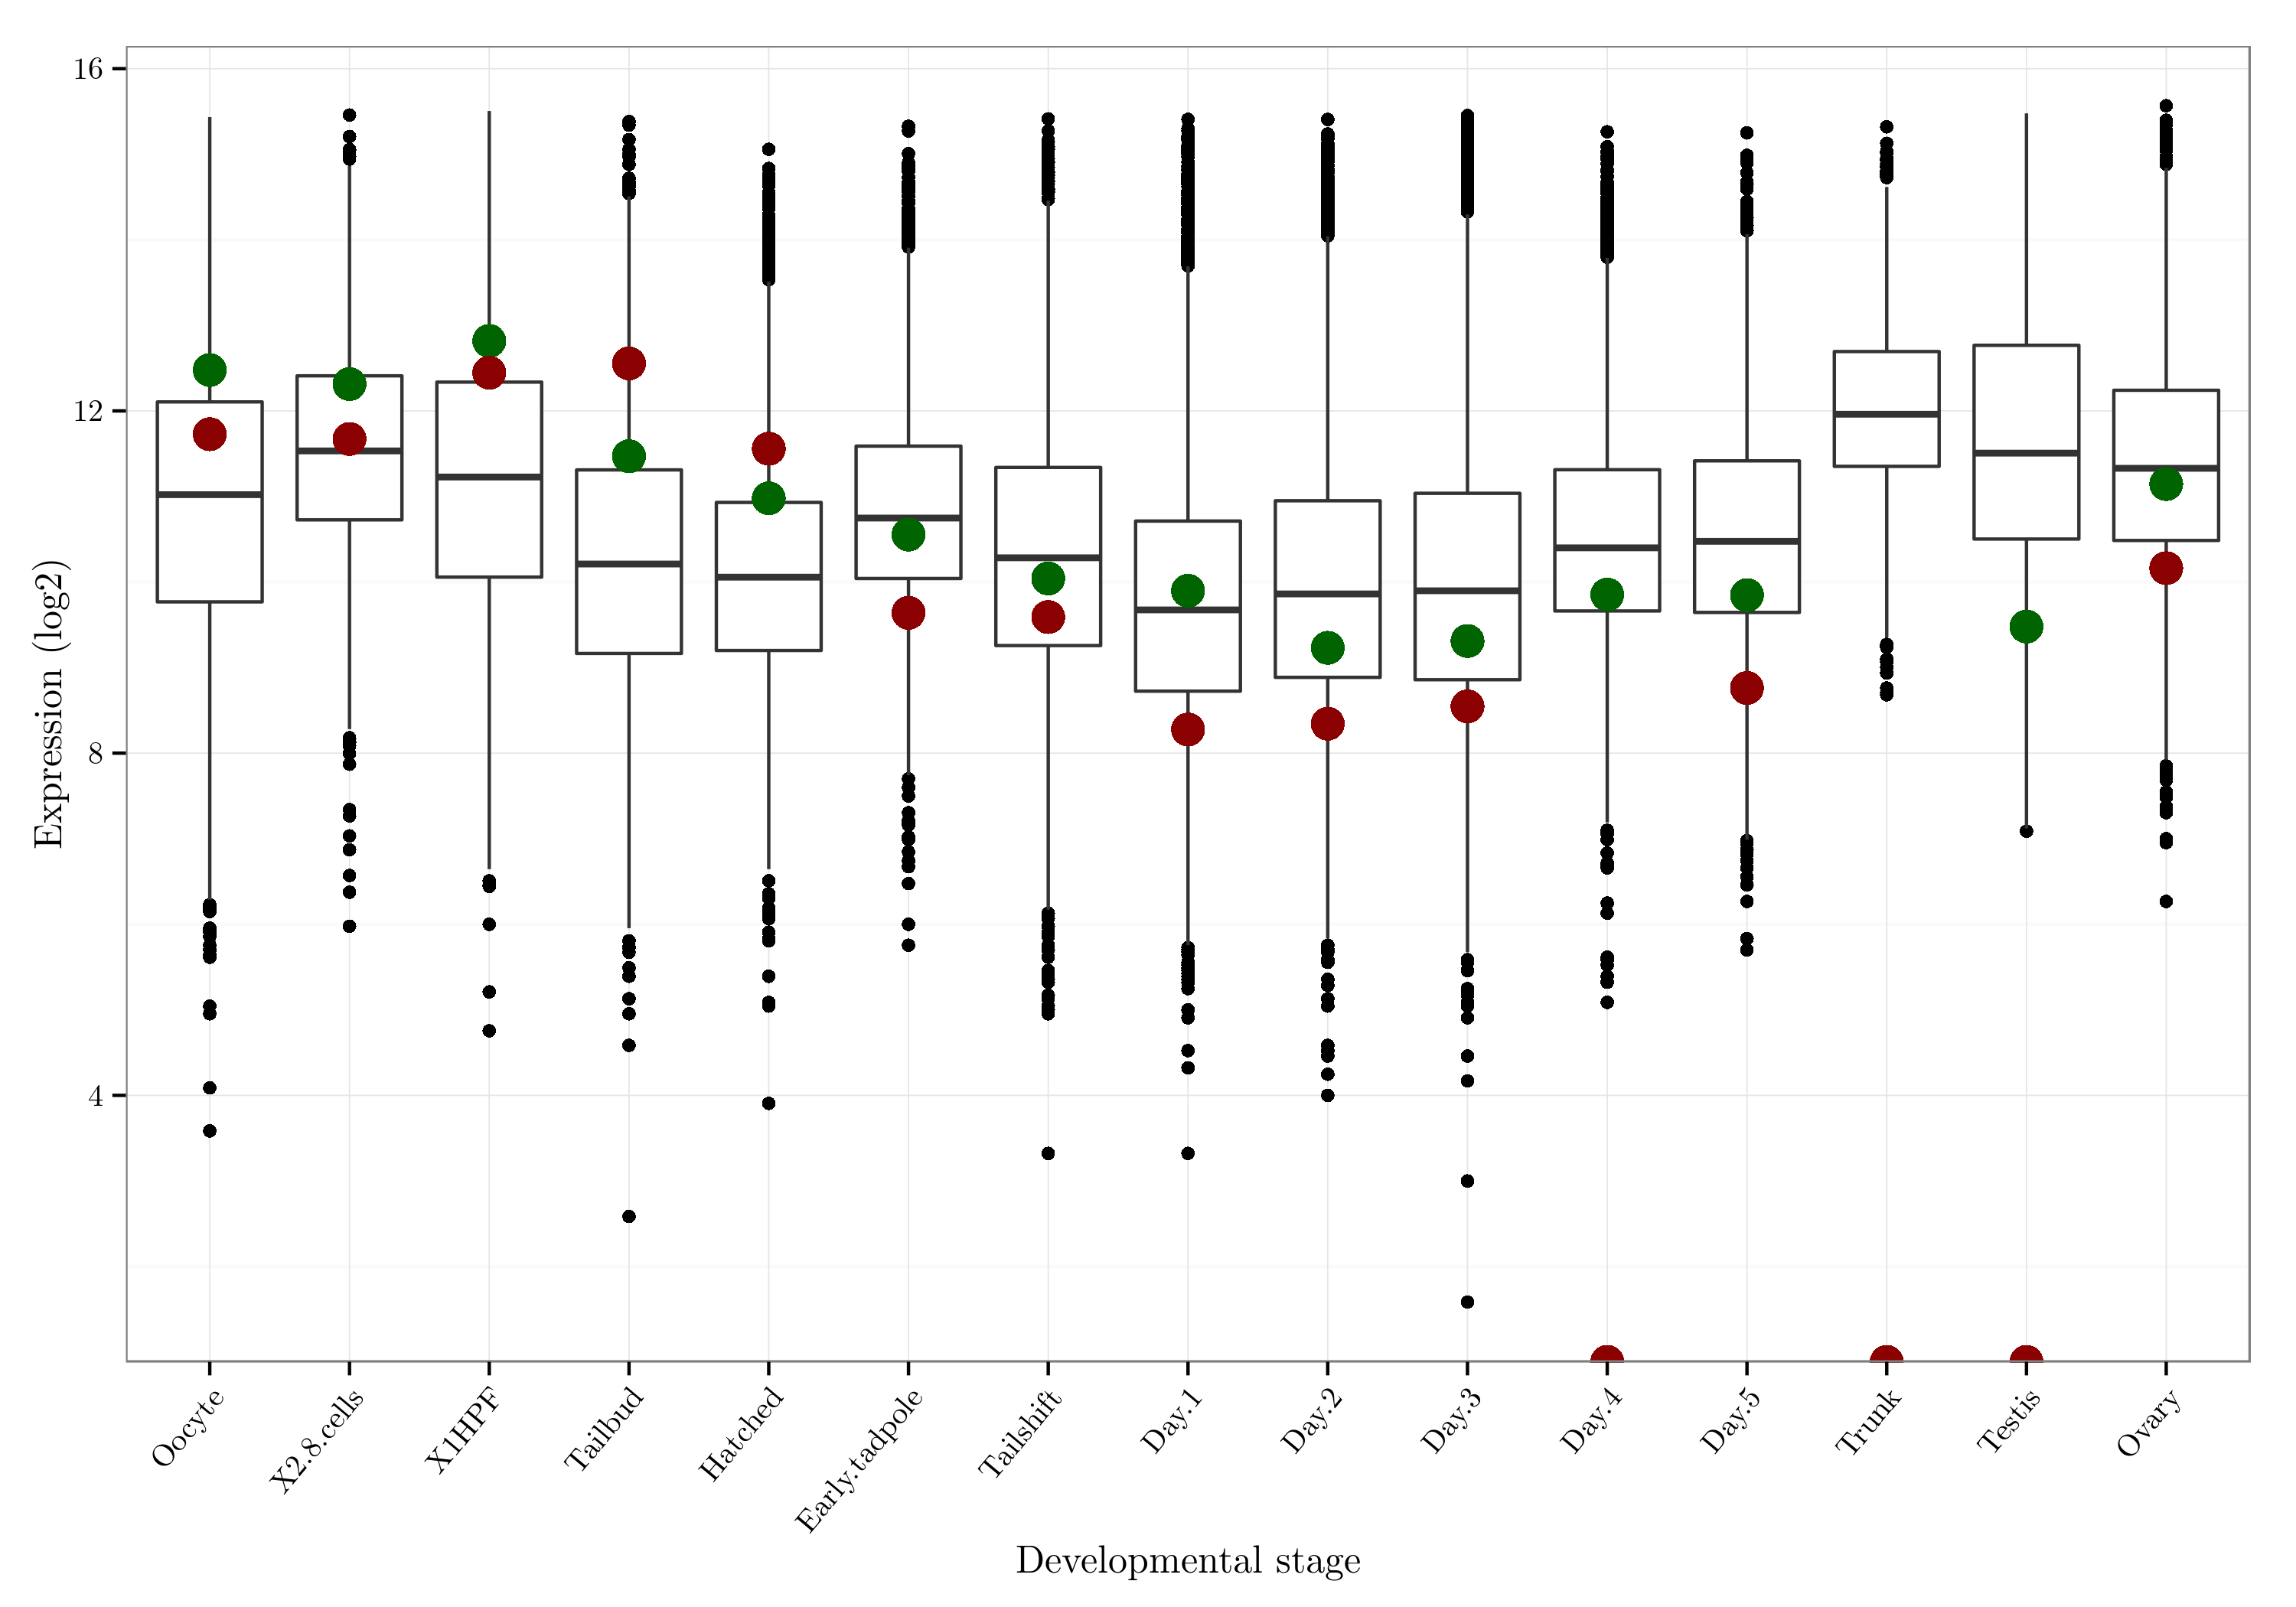
\includegraphics[width=0.9\textwidth]{pngs/E2F_expression_+allgenes.png}
		\caption[Expression levels of E2F factors during \textit{Oikopleura}'s development]
		{Expression levels of E2F factors during \textit{Oikopleura dioica}'s development.
			{
				\footnotesize
					Green: E2F1;
					Red: E2F7;
					Boxplots: All genes.
					Expression values transformed with a logarithm of base 2.
			}
		}
		\label{fig:E2F_expression}
	\end{figure}
	
	Despite the ubiquitous expression pattern of E2F TFs, differential binding and regulation of alternative genes can occur throughout development, leading to different biological outcomes. To investigate if E2F factors contribute to the use of different cell cycle modes through differential binding targets, we analyse ChIP-chip experiments of E2F1 and E2F7 TFs in dissected gonads of animals in Day 6 developmental stage of separate sexes.

	\subsection{Detection of E2F binding through ChIP-chip}
		\subsubsection{Validation of E2F antibodies}
		Antibodies used for immunoprecipitation of E2F TFs were validated by Western Blot (Figure \ref{fig:E2F_westerns}) and immunohistochemistry as previously published by Subramaniam \textit{et. al} \cite{Subramaniam2014} and found to detect the proteins in a specific manner.
		
		\begin{figure}[here]
			\setlength{\belowcaptionskip}{5pt}
			\centering
			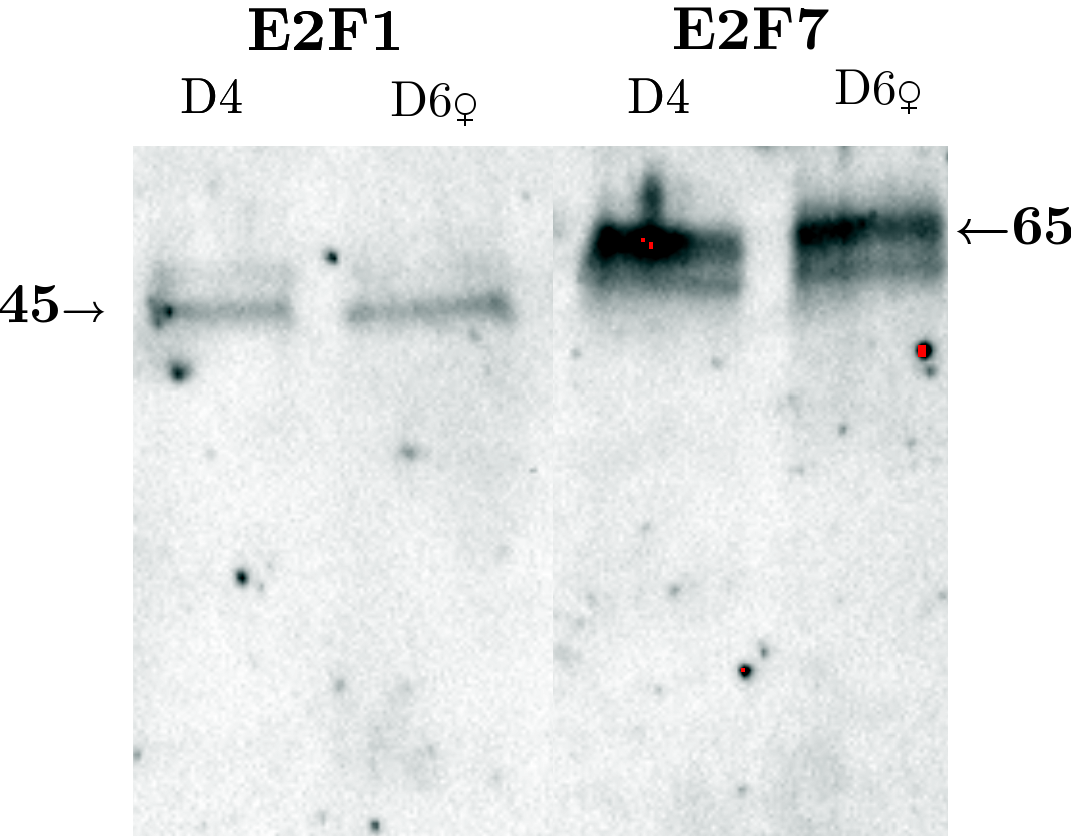
\includegraphics[width=0.4\textwidth]{pngs/E2Fs_western.png}
			\caption[Detection of E2F proteins in two developmental stages of\textit{Oikopleura}]
			{Detection of E2F proteins in two developmental stages of\textit{Oikopleura dioica}.
				{\footnotesize 
					Molecular weight in kDa.
				}
			}
			\label{fig:E2F_westerns}
		\end{figure}
	
		\subsubsection{Genomic context of E2F binding sites}
		When conducting genome-wide analysis of features of interest (\textit{e.g.} TF binding sites, cis-regulatory elements), the distribution of genetic and regulatory elements that make the background features of the genome under analysis mirror its architecture and can influence the statistical significance of the distribution of features of interest when compared with the background.
		
		\textit{Oikopleura dioica} possesses the most compact genome known yet for a chordate organism \cite{Denoeud2010a}, with reduced intergenic and intronic space, and enlarged proportion of coding sequence when compared with other model systems, both invertebrates and vertebrates (Figure \ref{fig:genome_background}).
	
		\begin{figure}[here]
			\setlength{\belowcaptionskip}{5pt}
			\centering
			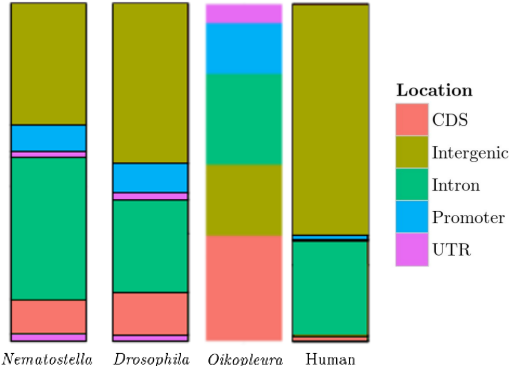
\includegraphics[height=0.3\textwidth]{pngs/species_genome2.png}
			\caption[Comparison of the distribution of genomic features in \textit{Oikopleura} and other animal models]
			{Comparison of the relative distribution of genomic features in \textit{Oikopleura dioica} and other animal models.
			{\footnotesize
				From left to right:
					\textit{Nematostella vectensis},
					\textit{Drosophila melanogaster},
					\textit{Oikopleura dioica},
					\textit{Homo sapiens}
				}
			}
			\label{fig:genome_background}
		\end{figure}
		
		The knowledge of the background of features in the genome of \textit{Oikopleura} will be useful when analysing the genomic context of E2F TF binding sites obtained by ChIP-chip. After preprocessing ChIP-chip data, putative binding sites of E2F TFs were obtained by selecting statistically significant ChIP-enriched regions (ChIP-ER) (see section \ref{subsection:methods_find_ChIP-ER} on methodology).
		
		Transcription factors are known to regulate gene expression by binding cis-regulatory elements (CREs) (\textit{e.g.} promoters, enhancers). Although CREs locate primarily in promoters and distal or intronic enhancer elements CITE, virtually every type of genomic feature can serve as a TF binding site. In \textit{Oikopleura}, E2F ChIP-ER were found to locate in close proximity to gene transcription start sites (TSS), regardless of the function of the TF (activator or repressor) and the developmental stage profiled (Figure \ref{fig:genomic context}a/b). 
				
		\begin{figure}
			\setlength{\belowcaptionskip}{5pt}
			\centering
			\begin{subfigure}[b]{1\textwidth}
				\centering
				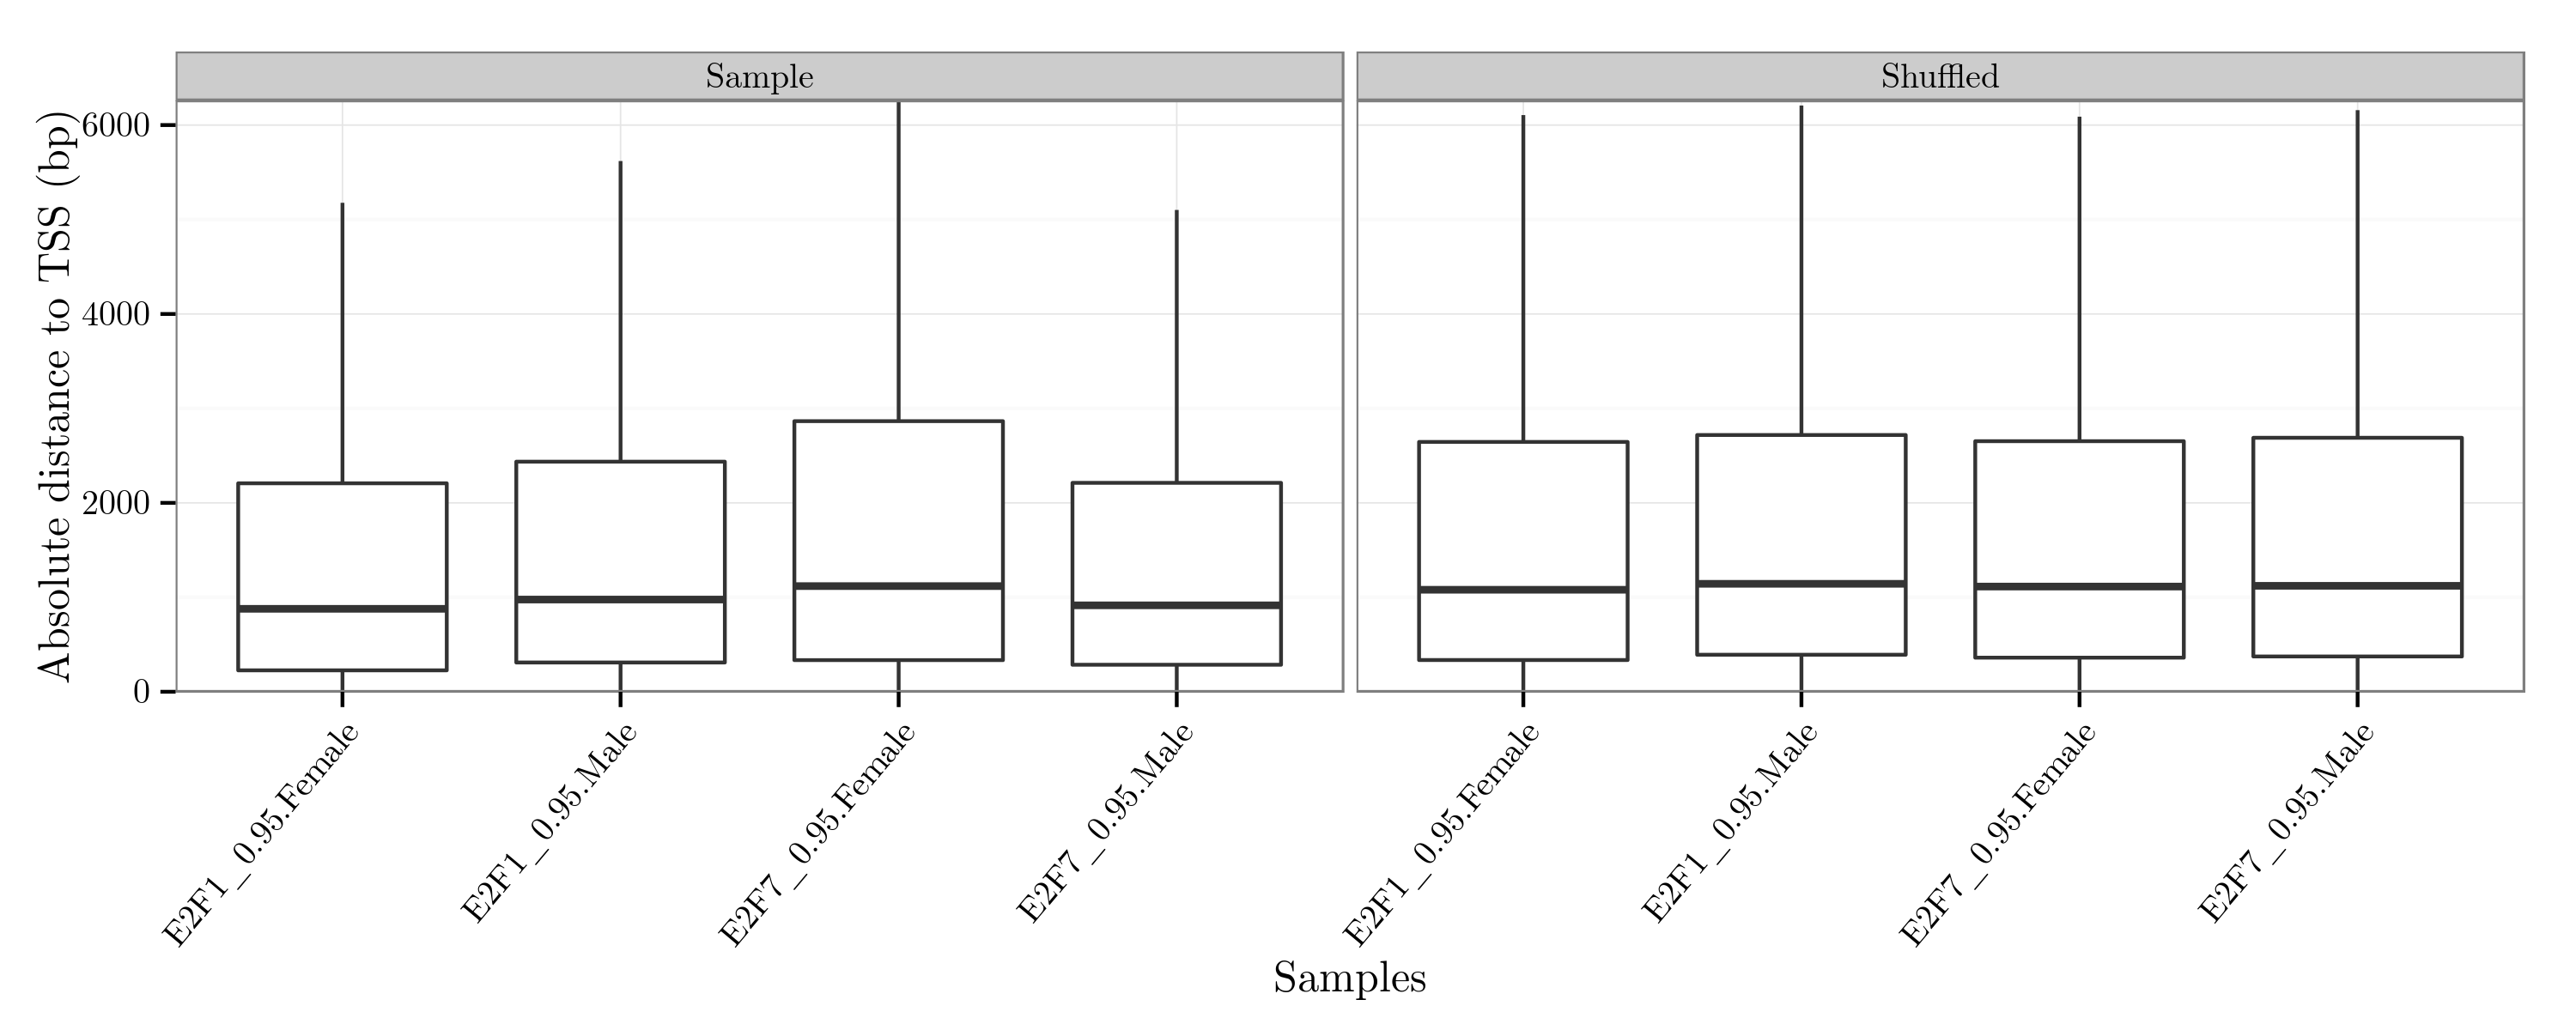
\includegraphics[width=1\linewidth]{pngs/E2F_distanceTSS_abs.png}
				\caption{Absolute distance of E2F ChIP-ER to the nearest gene TSS.}
			\end{subfigure}
			\begin{subfigure}[b]{1\textwidth}
				\centering
				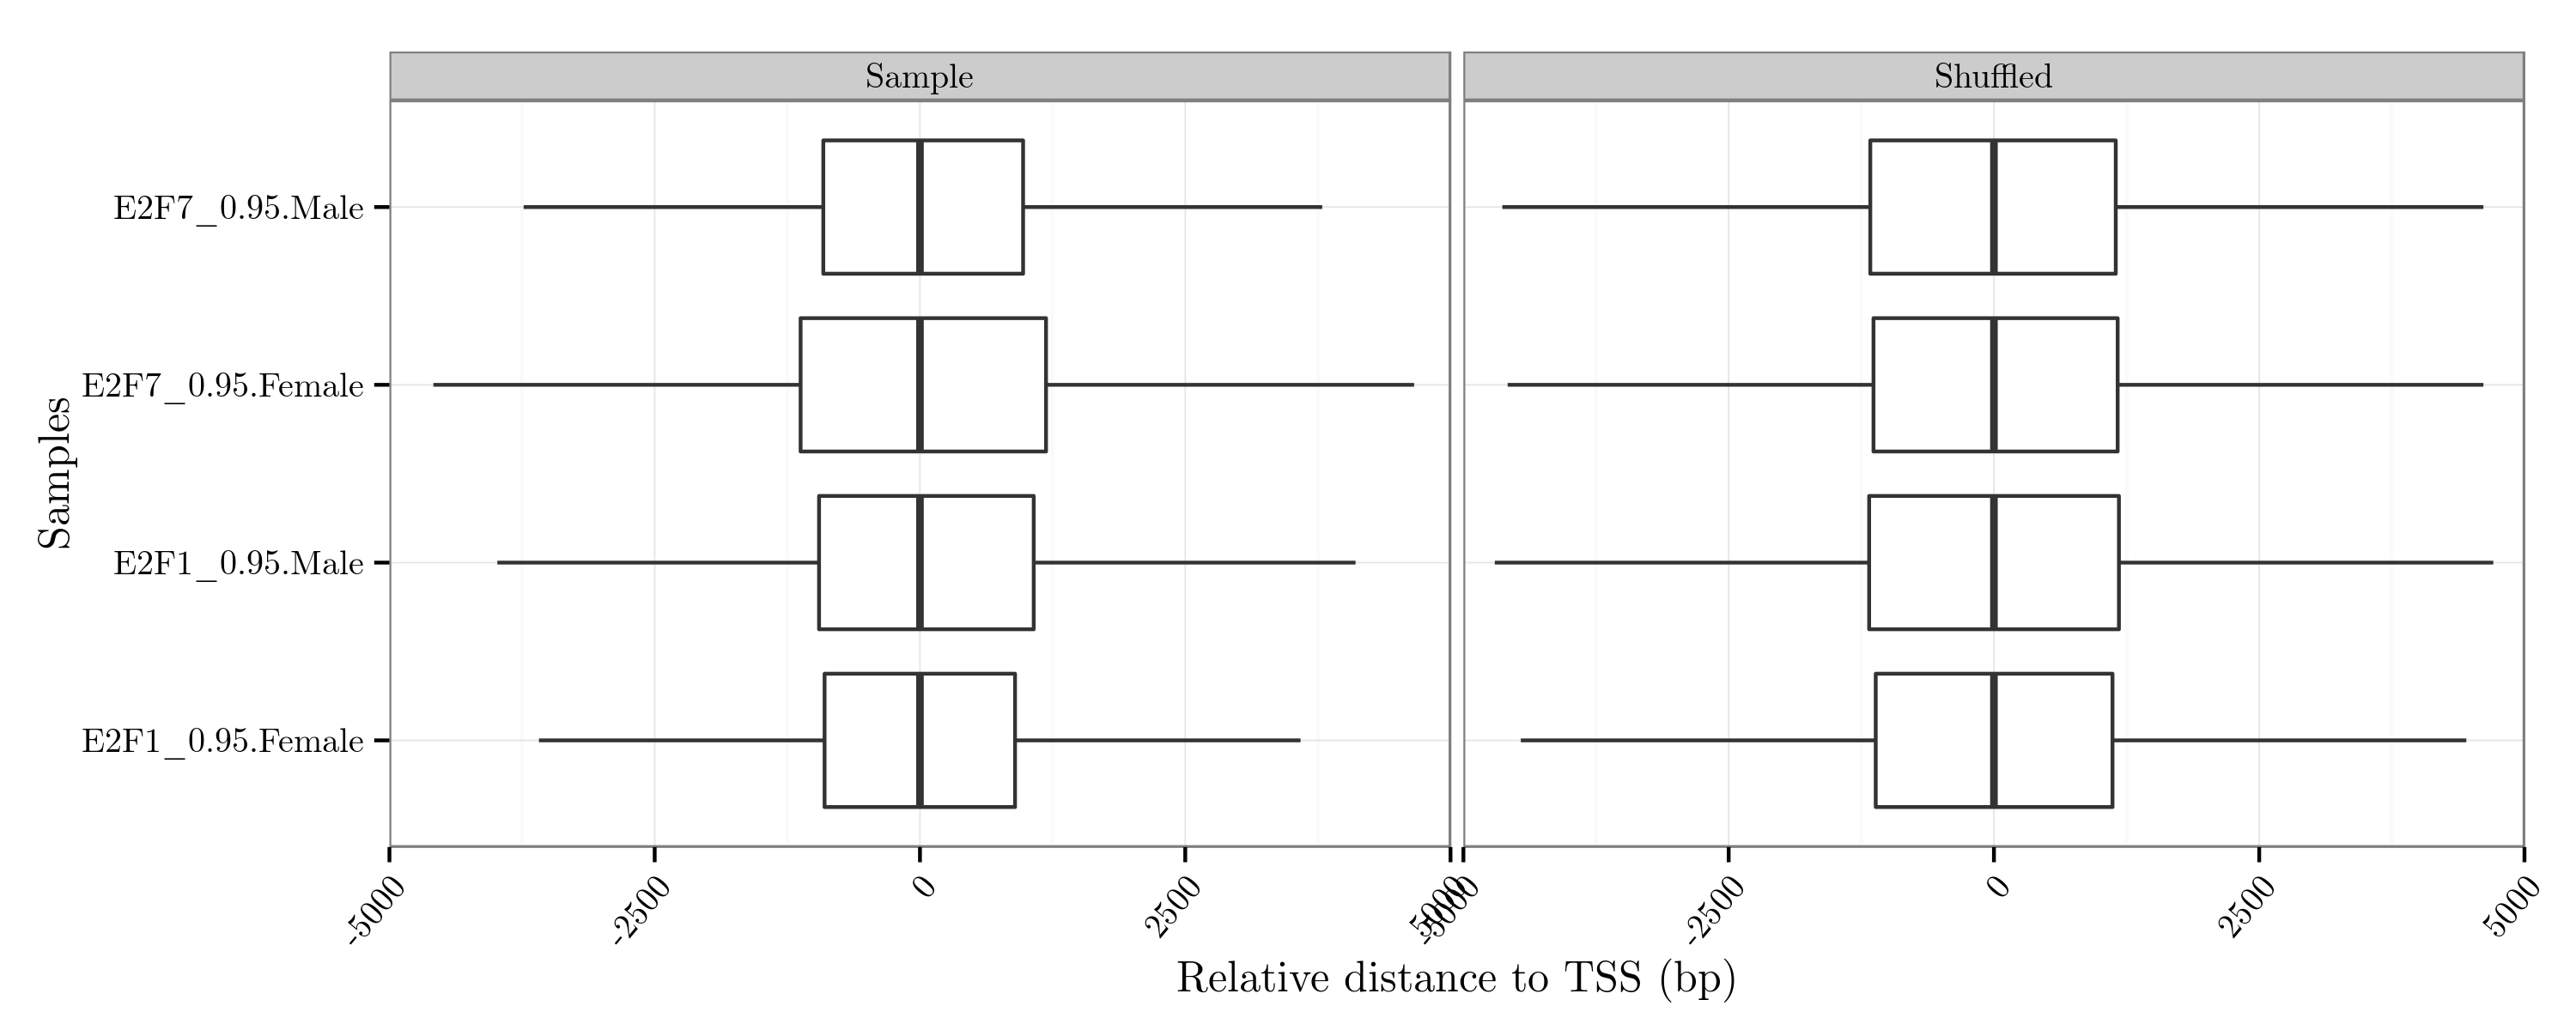
\includegraphics[width=1\linewidth]{pngs/E2F_distanceTSS_rel.png}
				\caption{Distance of E2F ChIP-ER relative to the nearest gene TSS.}
			\end{subfigure}
			\begin{subfigure}[b]{1\textwidth}			
				\centering
				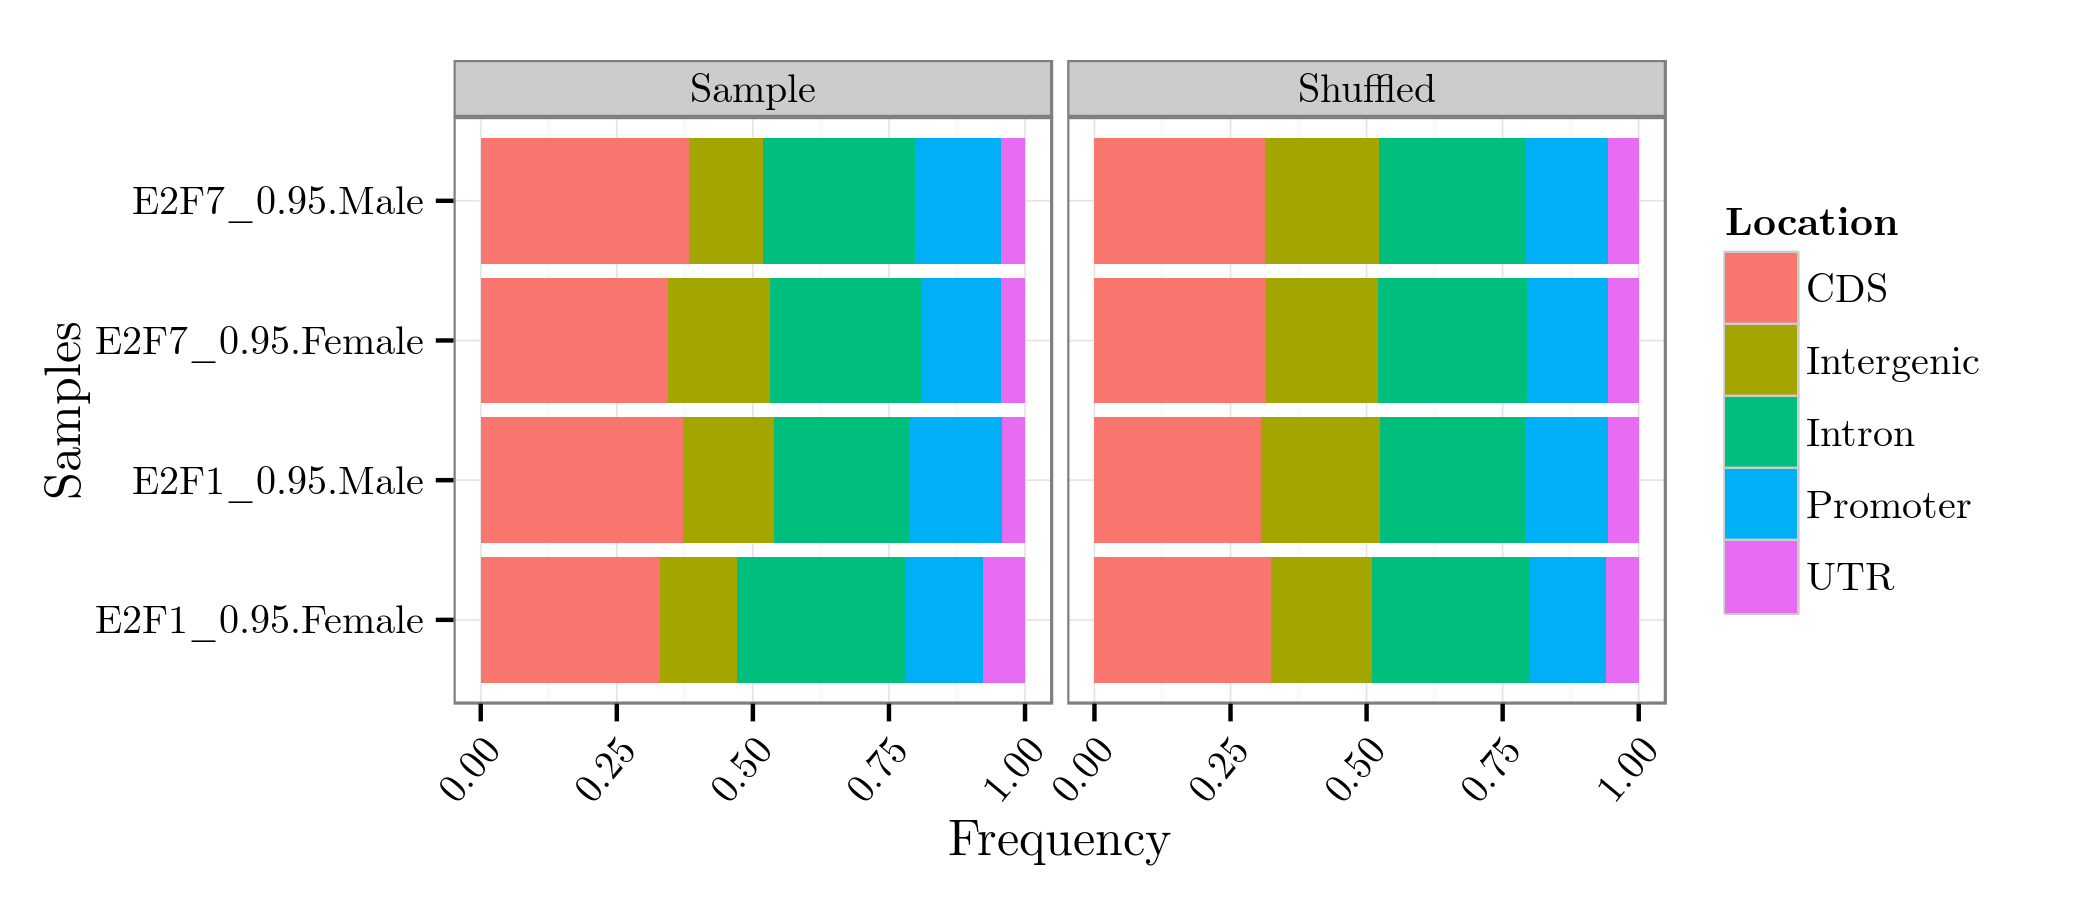
\includegraphics[width=0.9\textwidth]{pngs/E2F_genomicLocation.png}
				\caption{Location of E2F ChIP-ERs in the genome.}
				\label{fig:genomic_location}
			\end{subfigure}
			\caption[Genomic context of E2F ChIP-enriched regions]
			{Genomic context of \textit{Oikopleura} E2F ChIP-enriched regions.
				{\footnotesize
					Shuffled data has same number and widths as ChIP-ERs.
				}
			}
			\label{fig:genomic context}
		\end{figure}
		
		When comparing the distribution of observed distances with randomly positioned data of same size and widths, no statistically significant differences were found. Furthermore in both observed and randomized data the median distance to the nearest TSS coincided with it, revealing the structural constraints imposed by the compact genome. Nevertheless, the width of the distributions of observed data were smaller than the randomized, showing some propensity for the observed data to cluster around gene TSSs.
		
		Regarding the type of genomic features which E2F putatively bind, a considerable portion of ChIP-ERs overlaps regions of coding sequence(CDS) (Figure \ref{fig:genomic context}c) - this was unexpected, due to the general sequence constrains (\textit{e.g.} in terms of codon usage) of CDS and due to the preferential location of TF binding sites in non-coding regions. The portion of ChIP-ERs overlaping CDS was in some cases higher than expected by chance. This could be explained  by the combination of close proximity of ChIP-ERs to gene TSS and the wideness of ChIP-ER provided by the microarray technology, making overlaps between ChIP-ERs and CDS more likely.
		
		Overall, the distribution of ChIP-ERs in the \textit{Oikopleura} genome for both TFs in both stages analysed (Figure \ref{fig:genomic context}c) resembles what is expected by chance, and once again represents the constrains imposed by the genomic architecture.

		\subsubsection{Insights into the mechanism of E2F binding}
		
		Transcription factors are by definition sequence-specific DNA-binding proteins, but TF binding has also been shown to be constrained by the local epigenetic state of chromatin. Current findings have shown that the existence of a balance between local epigenetic context and TF sequence recognition is a likely underlying the mechanism of TF binding at least for TFs important for development and differentiation.
		
		In E2F ChIP-ERs we found significantly overrepresented motifs that aligned significantly to the known E2F TF binding motif from vertebrate models (Figure \ref{fig:E2F_influence}a). The motifs found in \textit{Oikopleura} are shorter in length than the vertebrate. This could be due to the evolutionary distance to vertebrates and the rapid rate of evolution of \textit{Oikopleura}, and also by the fact that the vertebrate motif was acquired with a combination of techniques (\textit{e.g.} SELEX, ChIP) which allows higher resolution. Nevertheless, both E2F TFs of \textit{Oikopleura} seem to bind locations with sequence content conserved with vertebrates.
		%OTHER MOTIFS
		
		To explore the possibility that the local epigenetic environment conditions the binding of the E2F TFs, we investigated the distribution of E2F ChIP-ERs in relation to a genome-wide annotation of chromatin states based on histone modifications (P. Navratilova, G. Danks and E. Thompson, unpublished data). This annotation provides 15 discrete epigenetic states based on genome-wide profiles of 19 histone modification marks obtained by ChIP-chip (Figure \ref{fig:E2F_influence}b). 
		
		The pattern of distribution of chromatin states in ChIP-ERs is highly similar within the same developmental stage as opposed to the the expectation that TFs with the same regulatory function (activator, repressor) would be more similarly constrained and more similarly likely to transform the epigenetic environment. E2F ChIP-ERs didn't show any preference for a particular local epigenetic signature (Figure \ref{fig:E2F_influence}c). A possible explanation lies on the wideness of ChIP-ERs provided by the microarray technology in a very compact genome, for if a high proportion of ChIP-ERs overlap with many chromatin states, the overal resolution would drop, reflecting mostly the overall landscape of chromatin states and epigenetic regulation within a particular developmental stage. It is also possible that E2F factors are not particularly sensitive to or involved in remodeling the epigenetic lanscape by recruiting chromatin remodelers, such as known for TFs involved in core developmental functions and differentiation.
		
		\begin{figure}
			\setlength{\belowcaptionskip}{5pt}
			\centering
			\begin{subfigure}[b]{1\textwidth}
				\centering
				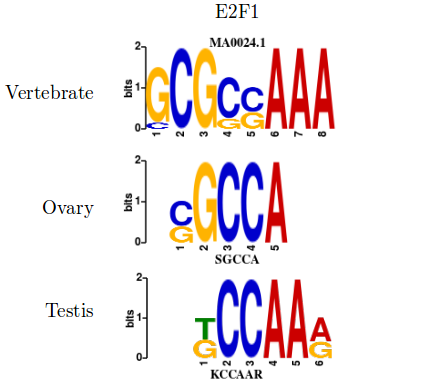
\includegraphics[width=0.45\textwidth]{pngs/E2F_motifs.png}
				\caption{Significant motifs found in E2F ChIP-ER that align with the known vertebrate E2F motif.}
			\end{subfigure}
			\begin{subfigure}[b]{1\textwidth}
				\centering
				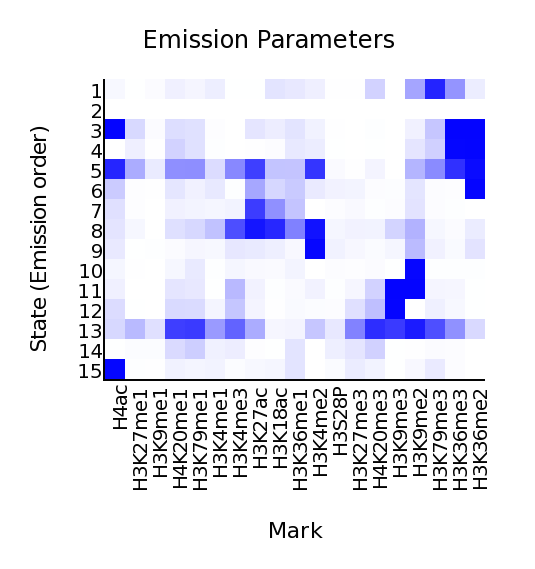
\includegraphics[width=0.5\linewidth]{pngs/ChromHMM_emissions_15.png}
				\caption{
					Composition of chromatin states based on histone modifications in \textit{Oikopleura dioica}.
					{\footnotesize 	Unpublished data kindly provided by P. Navratilova, G. Danks and E. Thompson.}
				}
			\end{subfigure}
			\begin{subfigure}[b]{1\textwidth}
				\centering
				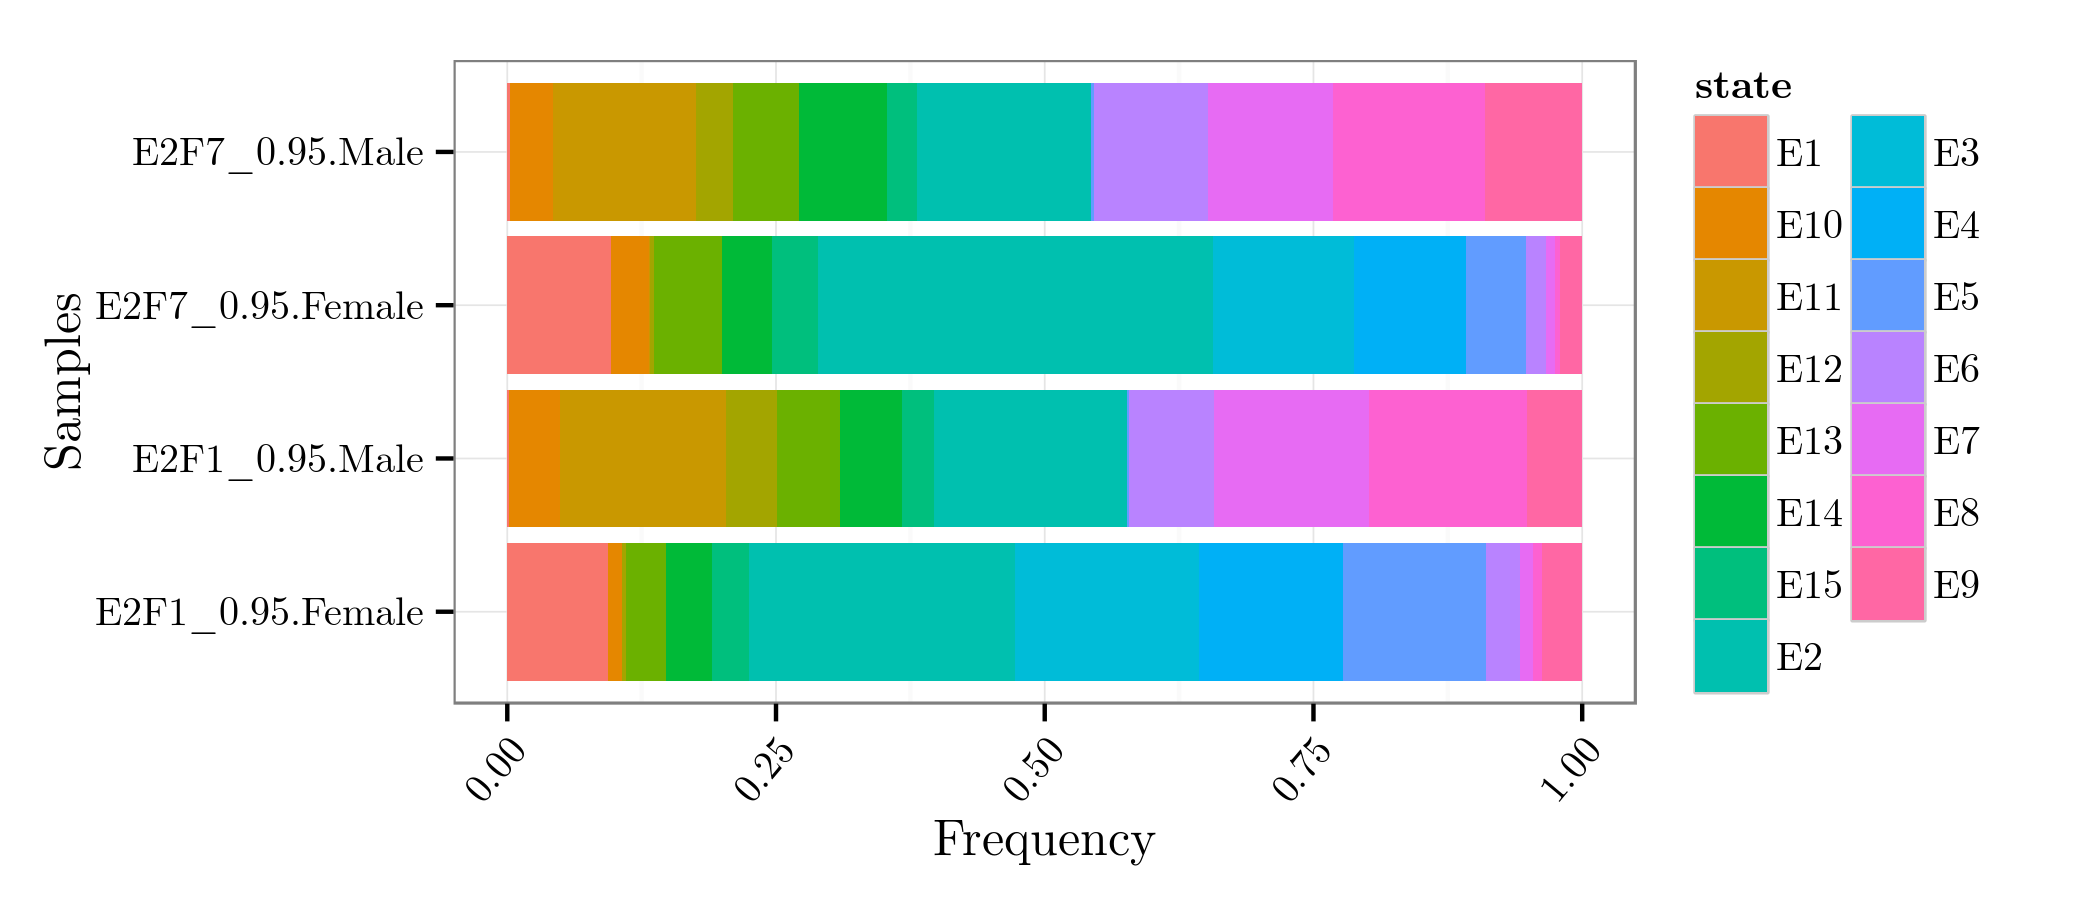
\includegraphics[width=1\linewidth]{pngs/E2F_chromatinAnnotation.png}
				\caption{Location of ChIP-ERs in the chromatin state annotation.}
			\end{subfigure}
			\caption[Influence of sequence specificity and local chromatin environment in E2F TF binding]
			{Influence of sequence specificity and local chromatin environment in E2F TF binding.}
			\label{fig:E2F_influence}
		\end{figure}
		
		\subsubsection{Spatial and temporal co-localization of E2F factors}
		E2F activator and repressor transcription factors are known to antagonize the effect of each other by regulating an overlapping set of genes in opposed ways CITE. To explore such relation in E2F TFs of \textit{Oikopleura}, we measured the degree of overlap between the two. Also in \textit{Oikopleura} ChIP-ERs of the activator (E2F1) and repressor (E2F7) showed high (45\% as maximum) spatial and temporal co-localization as seen by the overlap of ChIP-ERs within the same developmental stage (Figure \ref{fig:E2F_colocalization}a). From the ChIP-ERs of the two TFs that overlap within developmental stages, roughly half of them overlap between developmental stages (Figure \ref{fig:E2F_colocalization}b), showing that there is indeed a high degree of overlap between the genomic regions bound and likely the set of genes regulated.
    	
		\begin{figure}[here]
			\setlength{\belowcaptionskip}{5pt}
			\centering
			\begin{subfigure}[b]{1\textwidth}
				\centering
				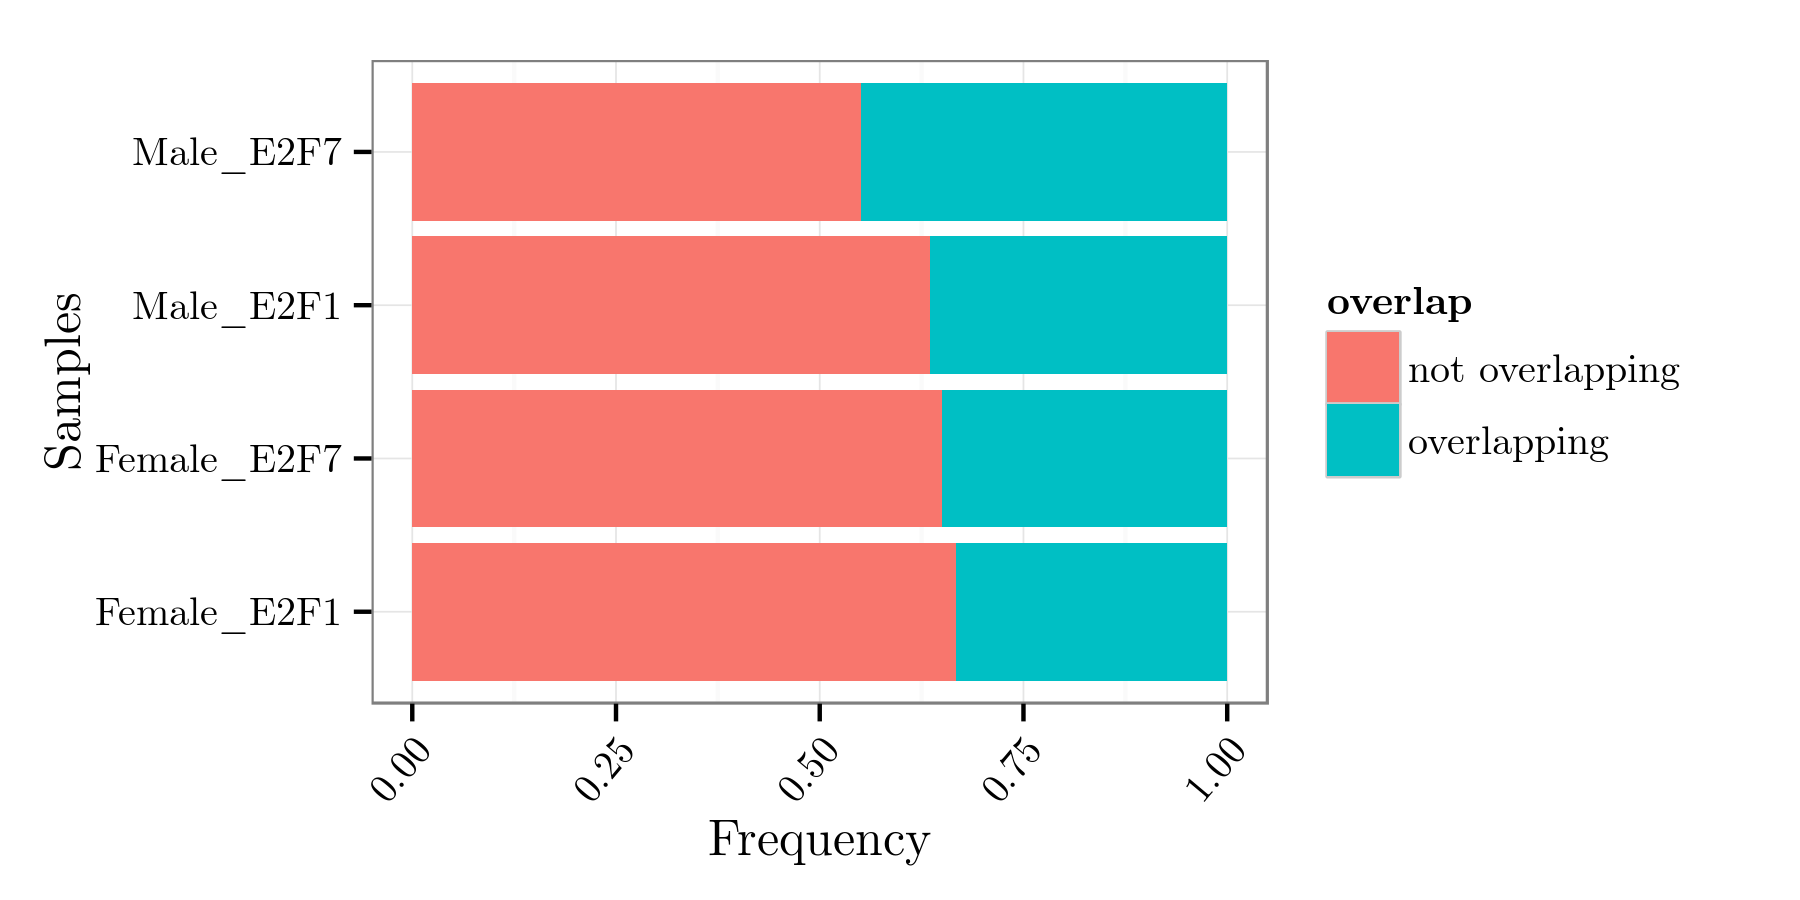
\includegraphics[width=0.75\linewidth]{pngs/E2F_overlap.png}
				\caption{Portion of ChIP-ERs that are shared (overlap) between transcription factors within the same developmental stage.}
			\end{subfigure}
			\begin{subfigure}[b]{1\textwidth}
				\centering
				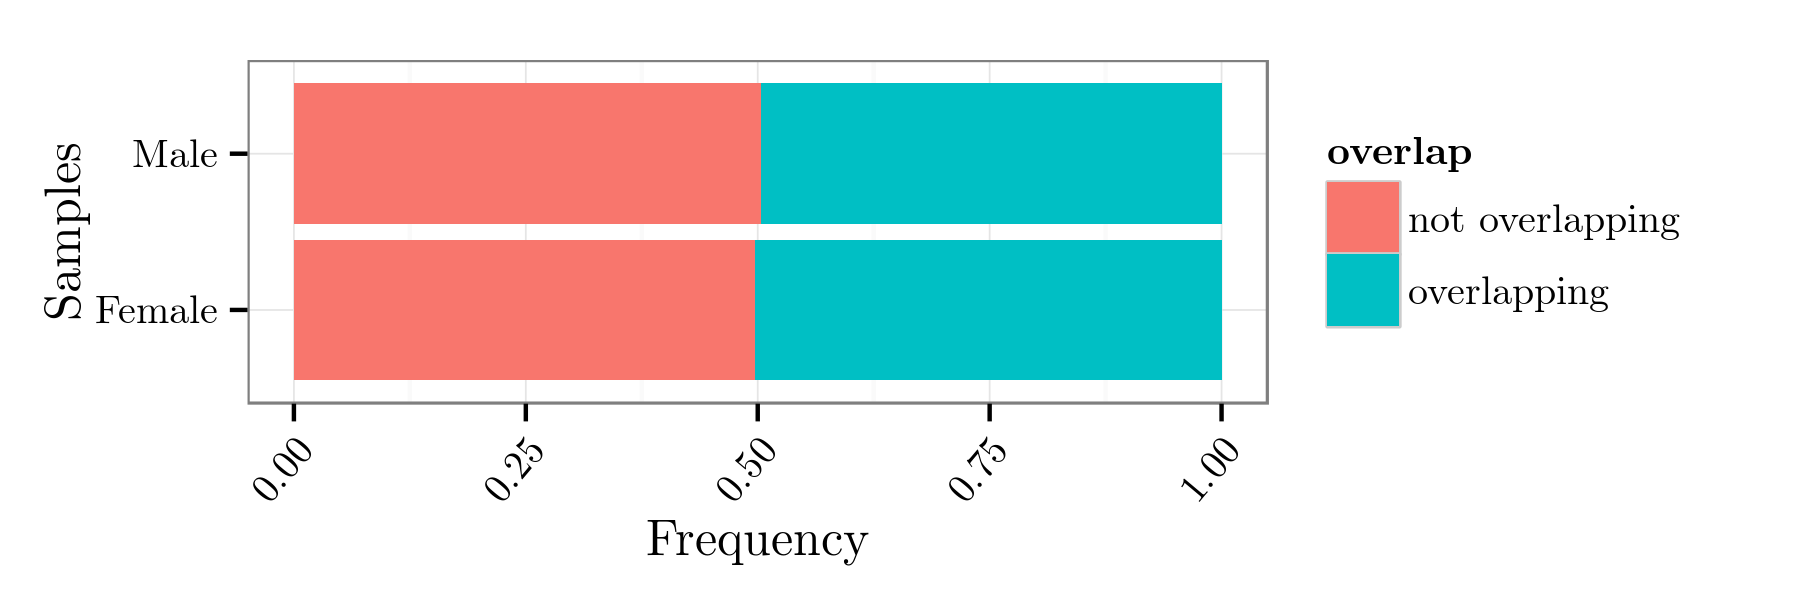
\includegraphics[width=0.75\linewidth]{pngs/E2F_overlap_overlaps.png}
				\caption{Portion of shared (overlapping) ChIP-ERs between transcription factors that also overlap between developmental stages.}
			\end{subfigure}
			\caption[Portion of E2F ChIP-ERs shared within and between developmental stages]
			{Portion of E2F ChIP-ERs shared (overlapping) within and between developmental stages.}
			\label{fig:E2F_colocalization}
		\end{figure}
		
		However, since ChIP experiments were performed on tissues with unsynchronised nuclei, the signal from the ChIP experiment most likely gives an overall picture of the binding of E2F TFs during this developmental stage by masking the possibly more subtle changes in E2F action during a cell cycle, rather than providing an accurate description of events inside an "ideal nucleus".
		
	\subsection{Putative E2F regulated genes (target genes)}
		Transcription factor binding has the function of altering the expression of genes. TFs binding diverse genomic locations have been shown to regulate genes near its binding site or in wide distances including different chromossomes. To attribute a putative binding event to the regulation of a gene, we assigned each ChIP-ER to the nearest transcription start site of a gene and said that this gene is regulated by this E2F ChIP-ER. This approach has the advantage that it assumes the less about the putative binding events, allowing genes to have multiple E2F regulatory elements in any genomic position. To study the functional properties of genes with an assigned ChIP-ER (from here on \textit{target genes}, for simplicity), we divided the genes into groups based on whether they were the targets of one TF exclusively or both in one of the tissues studied (ovary or testis) in Day 6 animals.
		
		\subsubsection{Gene ontology of target genes}
		From genes that are targets of both TFs within one tissue, a significant overrepresentation of genes whose biological processes is related with DNA replication and nucleotide metabolism was found (Figure \ref{fig:GO}). Other prominent overrepresented groups of gene ontology (GO) terms found among these genes were related with cell cycle regulation and progression, formation of protein-DNA complexes (with TFs overrepresented among these) and processes related with development of adult traits.
		
		\begin{figure}[here]
			\centering
			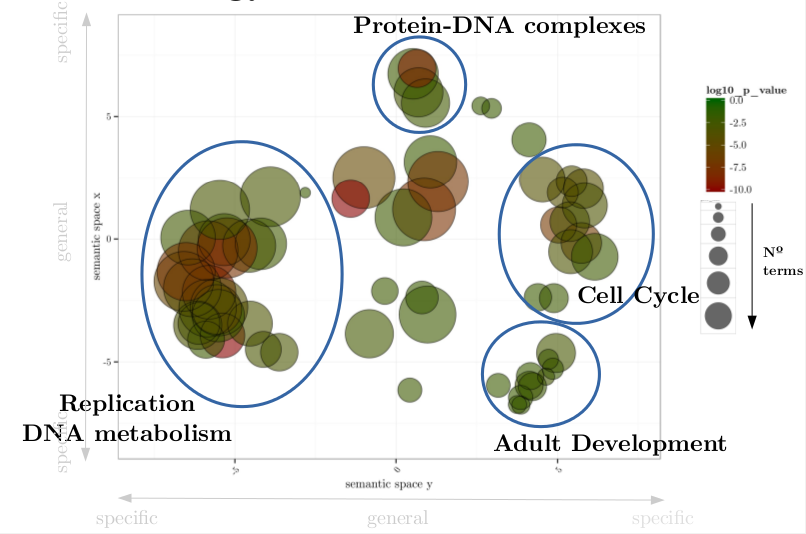
\includegraphics[width=1\textwidth]{pngs/E2F_overlap_overlaps_GO.png}
			\caption[Gene Ontology of genes putatively regulated by both E2F transcription factors]
			{Gene Ontology of genes putatively regulated by both E2F transcription factors in testis of animals in D6 developmental stage.
				{\footnotesize 
					Data spread over two semantic spaces (axis).
					Gene Ontology terms were nested within the same parent and the amount of terms clustered is shown by the area of the circle.
					Significance values are shown in a color spectra.
					Ovary of animals in the D6 developmental stage have a high degree of similarity.
				}
			}
			\label{fig:GO}
		\end{figure}
		
		Co-regulation of genes by the two TFs in the same development stage is likely due to the necessity of gaining fine control over the expression of these genes and highlights the importance of the E2F factors as key regulators of processes such as cell cycle progression and processes inherent to it (DNA replication, nucleic acid metabolism). Regulation of protein-DNA complexes and TFs is also not surprising due to the fact that regulation at the transcriptional level often exists in the form of gene regulatory networks of which TFs are the major regulatory force. Regardless, of the type of outcome from the action of a TF (activator or repressor), it is likely that other TFs will also be regulated accordingly. Since the stages of development studied here correspond to the last phase of \textit{Oikopleura}'s life cycle, general regulation of genes involved in biological processes important for acquisition of adult traits (\textit{e.g.} gametogenesis).
		
		Genes exclusively targeted by the E2F1 TF in the female gonad have a set of overrepresented GO terms associated with them highly similar to genes bound by both TFs, but in addition terms related with cytoskeletal activity. This could be related to the fact that during maturation of the female gonad oocytes expand their cytoplasmatic domain drastically, occupying a volume higher than the somatic part of the organism - such accomplishment requires extensive production and coordination of structural proteins in the cytoskeleton. In the analogous situation (exclusively bound E2F1 genes) in the male gonad, much fewer overrepresented GO terms were found. Of particular notice is the presence of the \textit{"metaphase/anaphase transition of mitotic cell cycle"} term, which is highly specific for M phase. The activation by E2F1 of genes involved in M phase is coincident with the resumption of cell cycles with mitotic phase which occurs in late maturation of the male gonad and during spermatogenesis (meiosis).
		
		Genes under exclusive action of E2F7 in the female gonad have a sparce and reduced set of overrepresented GO terms associated with them but where again the \textit{"metaphase/anaphase transition of mitotic cell cycle"} term stands out. The female gonad employs mainly endocycles throughout its maturation and it is foreseeable that genes involved in the promotion on M phase should be repressed to allow the endocycle. Genes exclusively bound by E2F7 in the male gonad have a rich set of overrepresented terms resembling the ones in Figure \ref{fig:GO}, but where terms such as \textit{"meioisis"} and terms related with transcription and RNA metabolism also appear. This could be due to the minimalistic nature of sperm when compared with the oocyte - sperm is mainly a carrier of genetic information in the form of the genome, as opposed to the oocyte which possesses maternal transcripts and reserve substances to support early development. E2F7 binding of genes involved in these functions could be contributing to their suppression.
		
		This mirror situation of genes involved in the same biological processes being activated or repressed inversely in the male and female gonads is indicative of the differences underlying the different cell cycle modes employed in the two tissues. However, although analysis of gene function through testing of under/overrepresented GO terms is useful, it assumes that genes have kept the same functional properties (biological process, cellular localization, molecular function) as the genes from which the terms were originally derived. Full lists of significantly overrepresented GO terms can be seen on appendix section \ref{appendix:GOterms}.		
		
		\subsubsection{Differences of expression in E2F target genes}
		The ultimate goal of transcription factor binding is to steer a developmental program in one direction by altering gene expression. Activator TFs positively influence gene expression whereas repressors have a negative effect by repressing or diminishing gene expression. We decided to explore the dynamics of gene expression in E2F target genes in \textit{Oikopleura} to see to which degree do they condition gene expression in the tissues analysed. 
		
    	There are major and significant changes of expression at the transcriptome level between ovary and testis tissue of animals in the D6 developmental stage (Figure \ref{fig:D6_expression}). Overall, there is a bias for genes being more highly expressed in the female gonad. In the male, a high fraction of genes are not expressed at all while being expressed at various levels in the ovary (note points stacked on x axis in Figure \ref{fig:E2F_targets_expression}a). This illustrates the intrinsic Biology of the maturing gonads - in the ovary, meiotic and nurse nuclei coexist and the expression values reflect genes expressed in both (possibly even different sets of genes).
		
		We tested the hypotesis that genes that are exclusively targeted by the E2F1 TF (activator) in a particular tissue would be more highly expressed in that tissue than in the other, and the inverse situation for genes exclusively targeted by E2F7 (repressor). There were no significant differences between the means of the distribution of these two groups in either tissue. However, a trend exists for genes that are bound by the repressor transcription factor (E2F7) in a stage to be less expressed in that stage and more in the other as shown by the inversion of position of smoothed and quantile lines in Figure \ref{fig:E2F_targets_expression}(b) and (c) between tissues.
		
		\begin{figure}[h!]
			\centering
			\begin{subfigure}{1\textwidth}
				\centering
				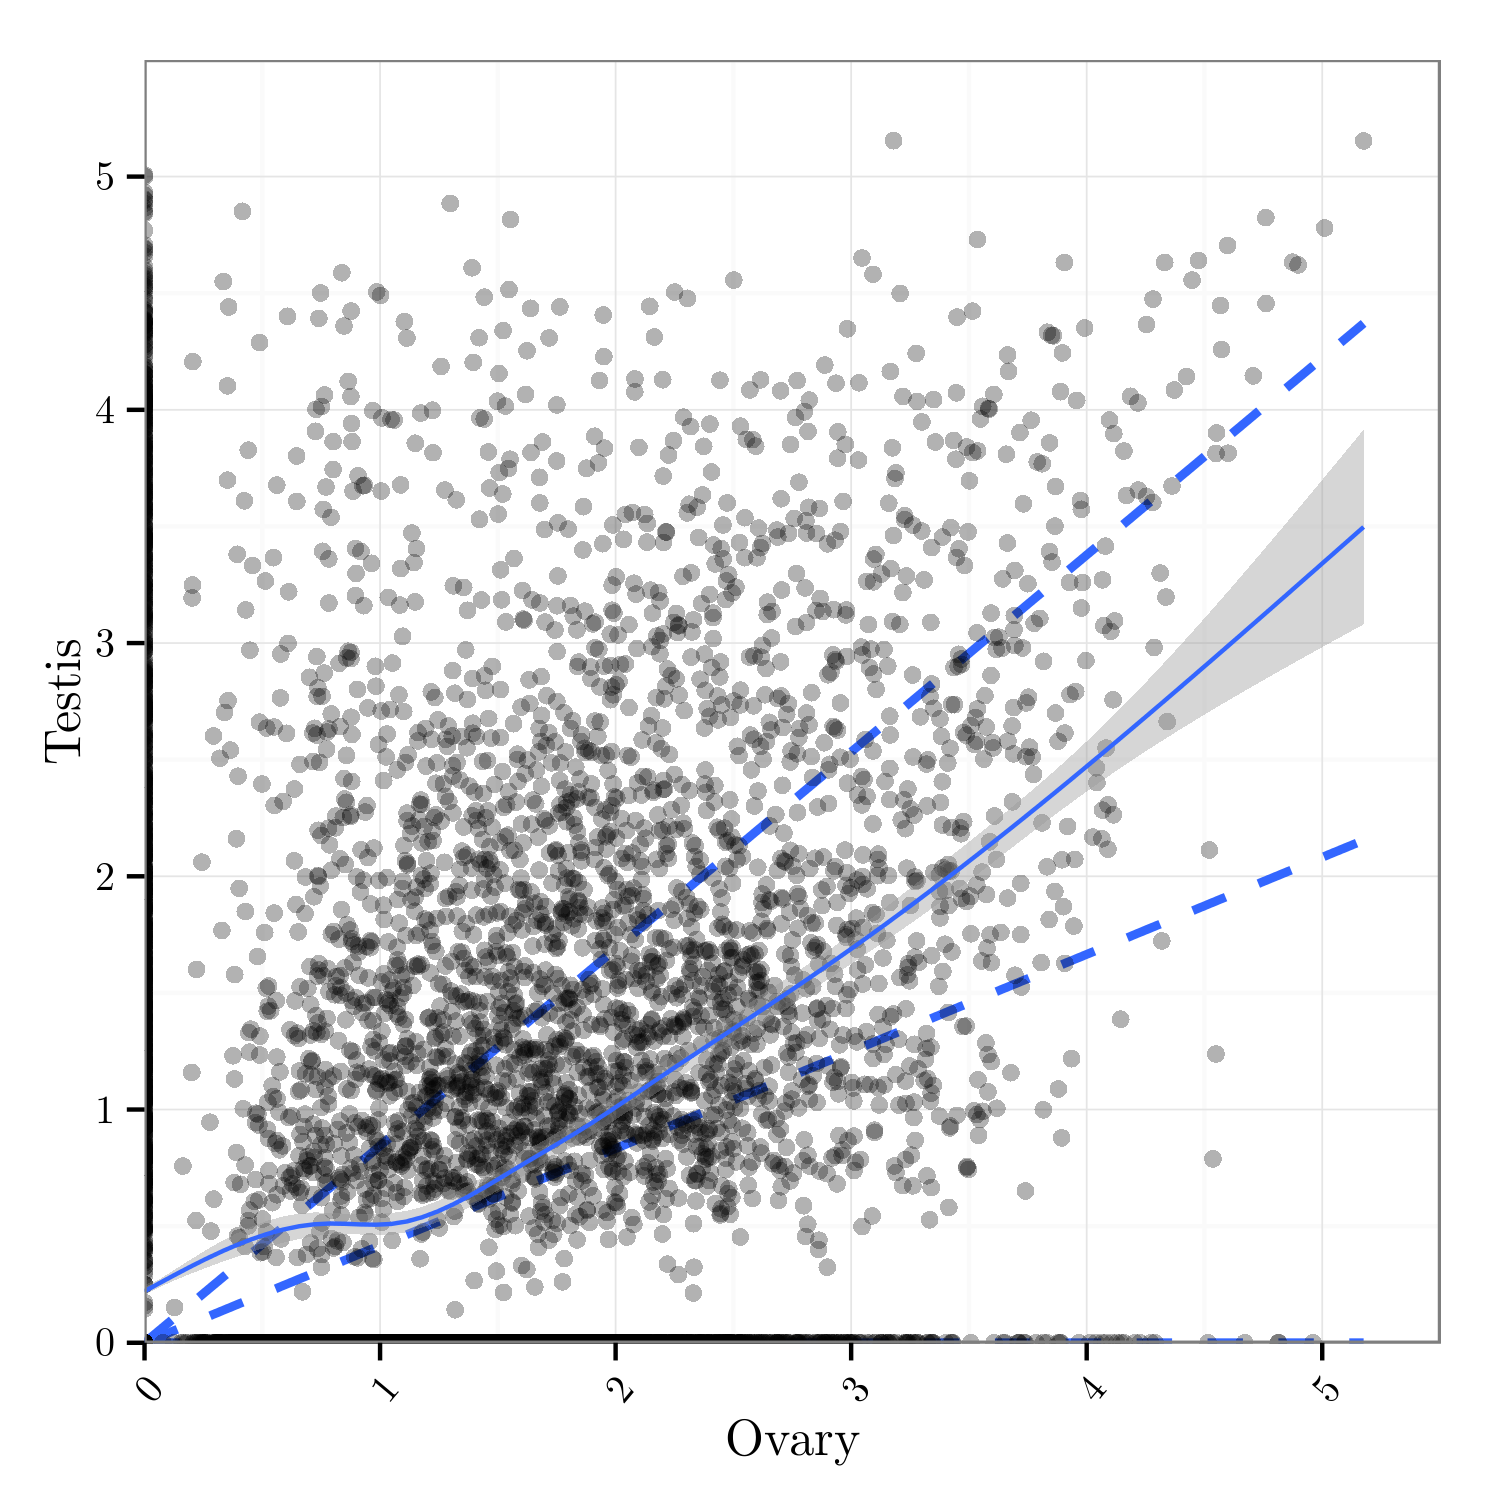
\includegraphics[width=0.5\textwidth]{pngs/D6_expression.png}
				\caption{Expression values of all genes in ovary and testis tissue of animals in the D6 developmental stage.}
			\end{subfigure}
			\begin{subfigure}{0.5\textwidth}
				\centering
				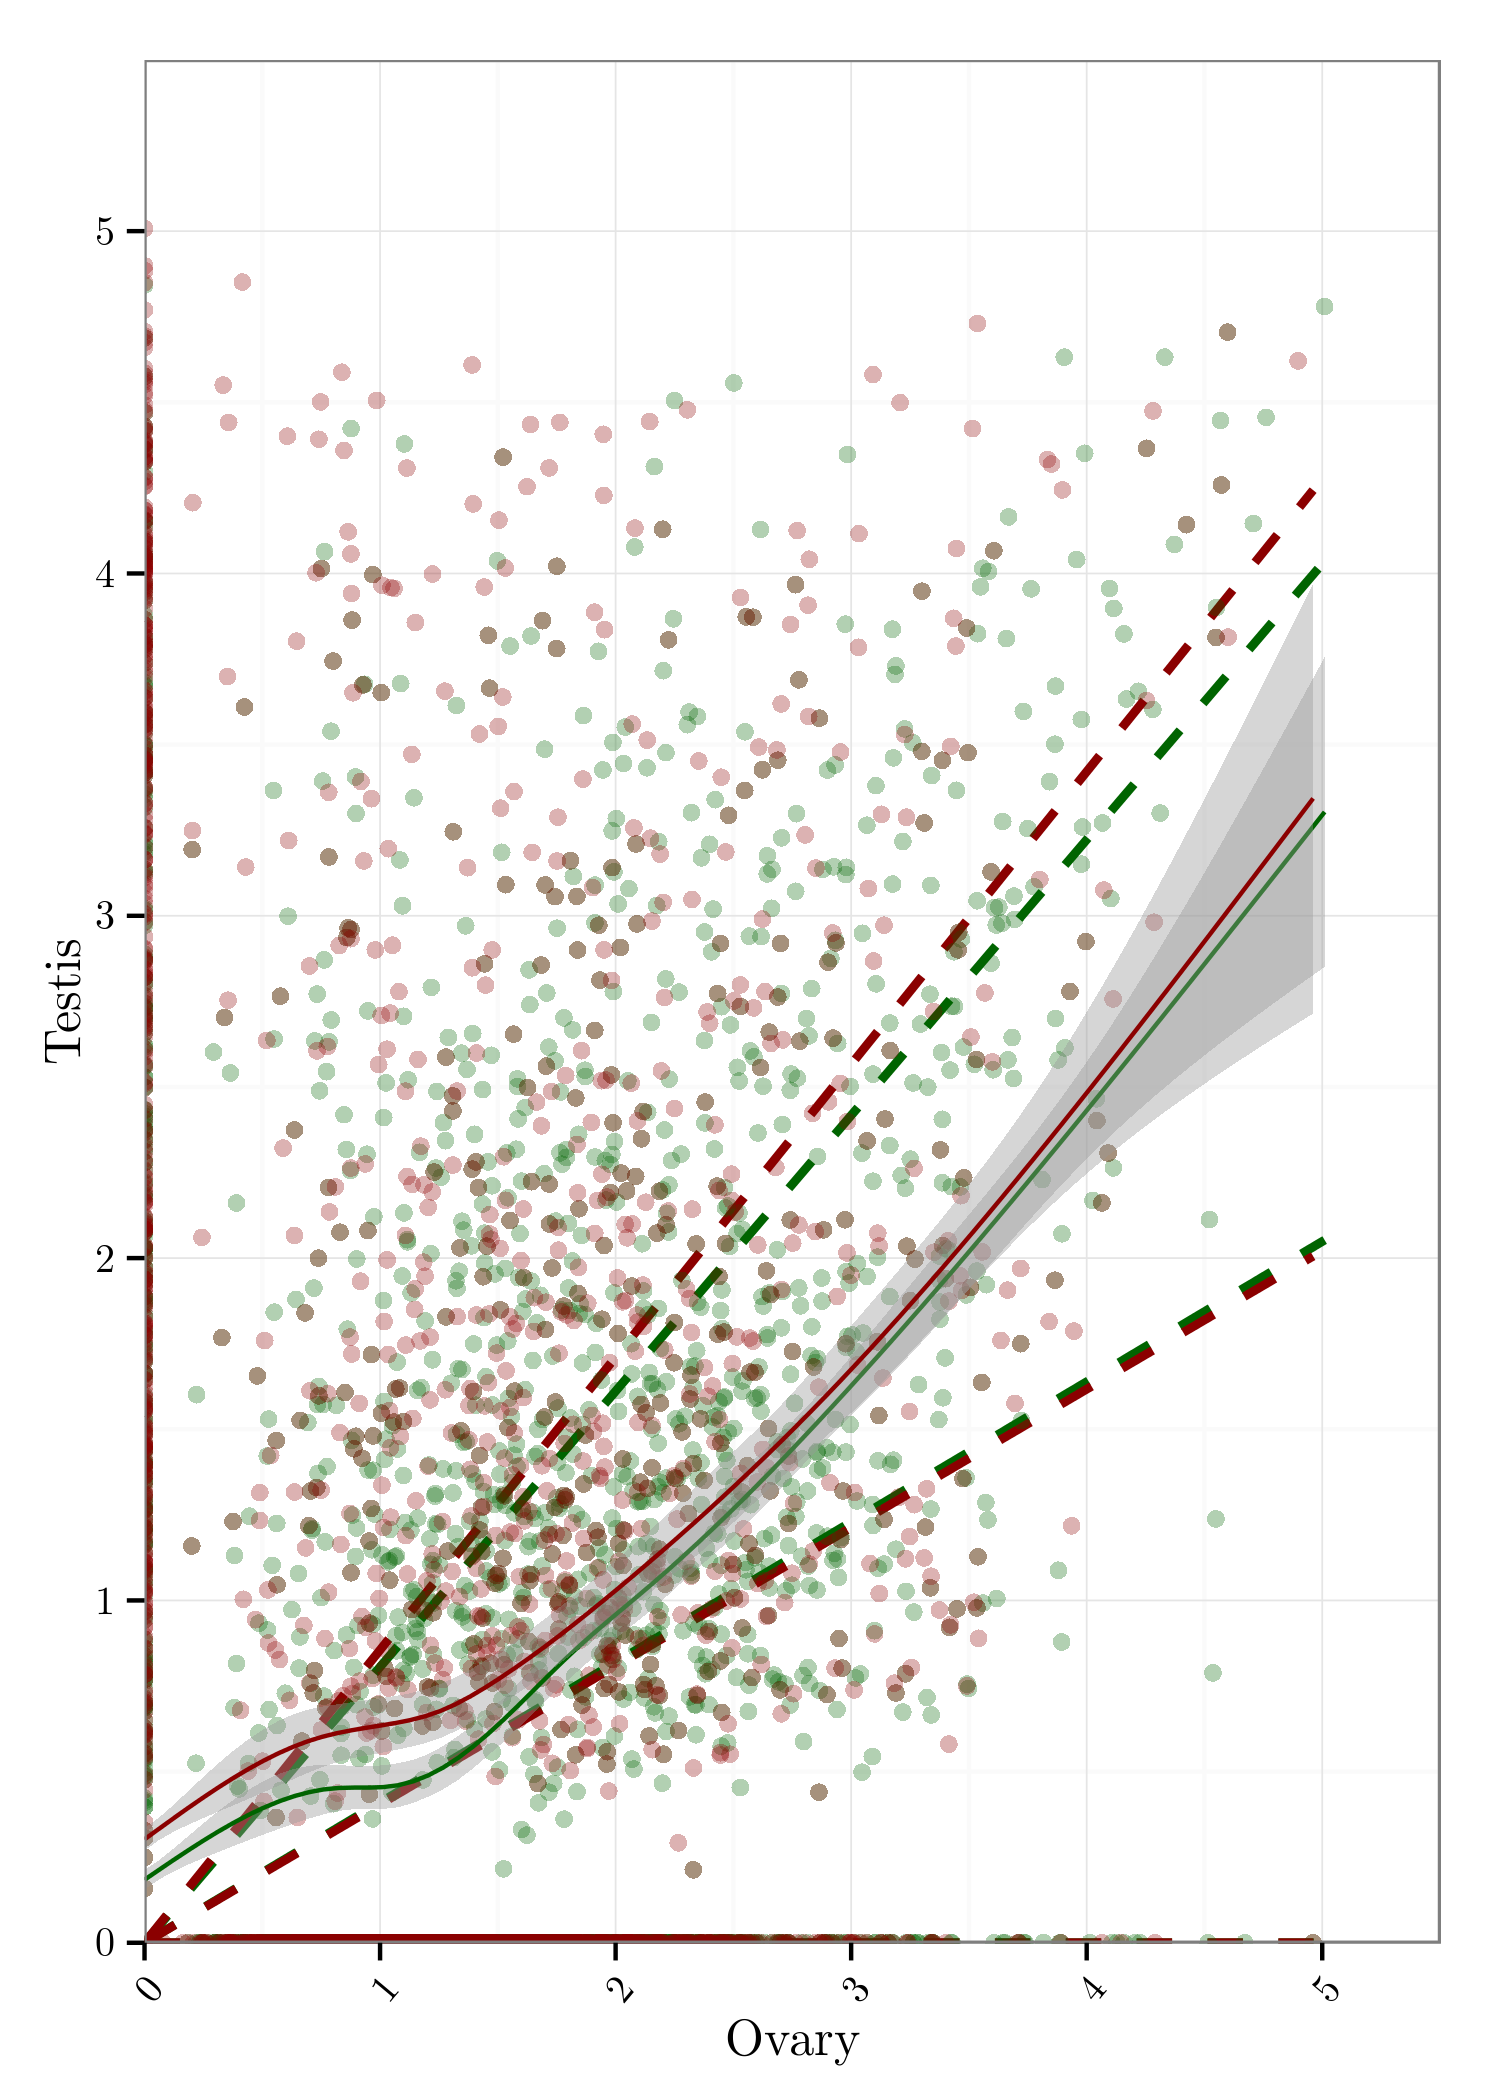
\includegraphics[width=1\linewidth]{pngs/E2F_specific_Female_expression.png}
				\caption{D6 Female developmental stage (Ovary).}
			\end{subfigure}%
			\begin{subfigure}{.5\textwidth}
				\centering
				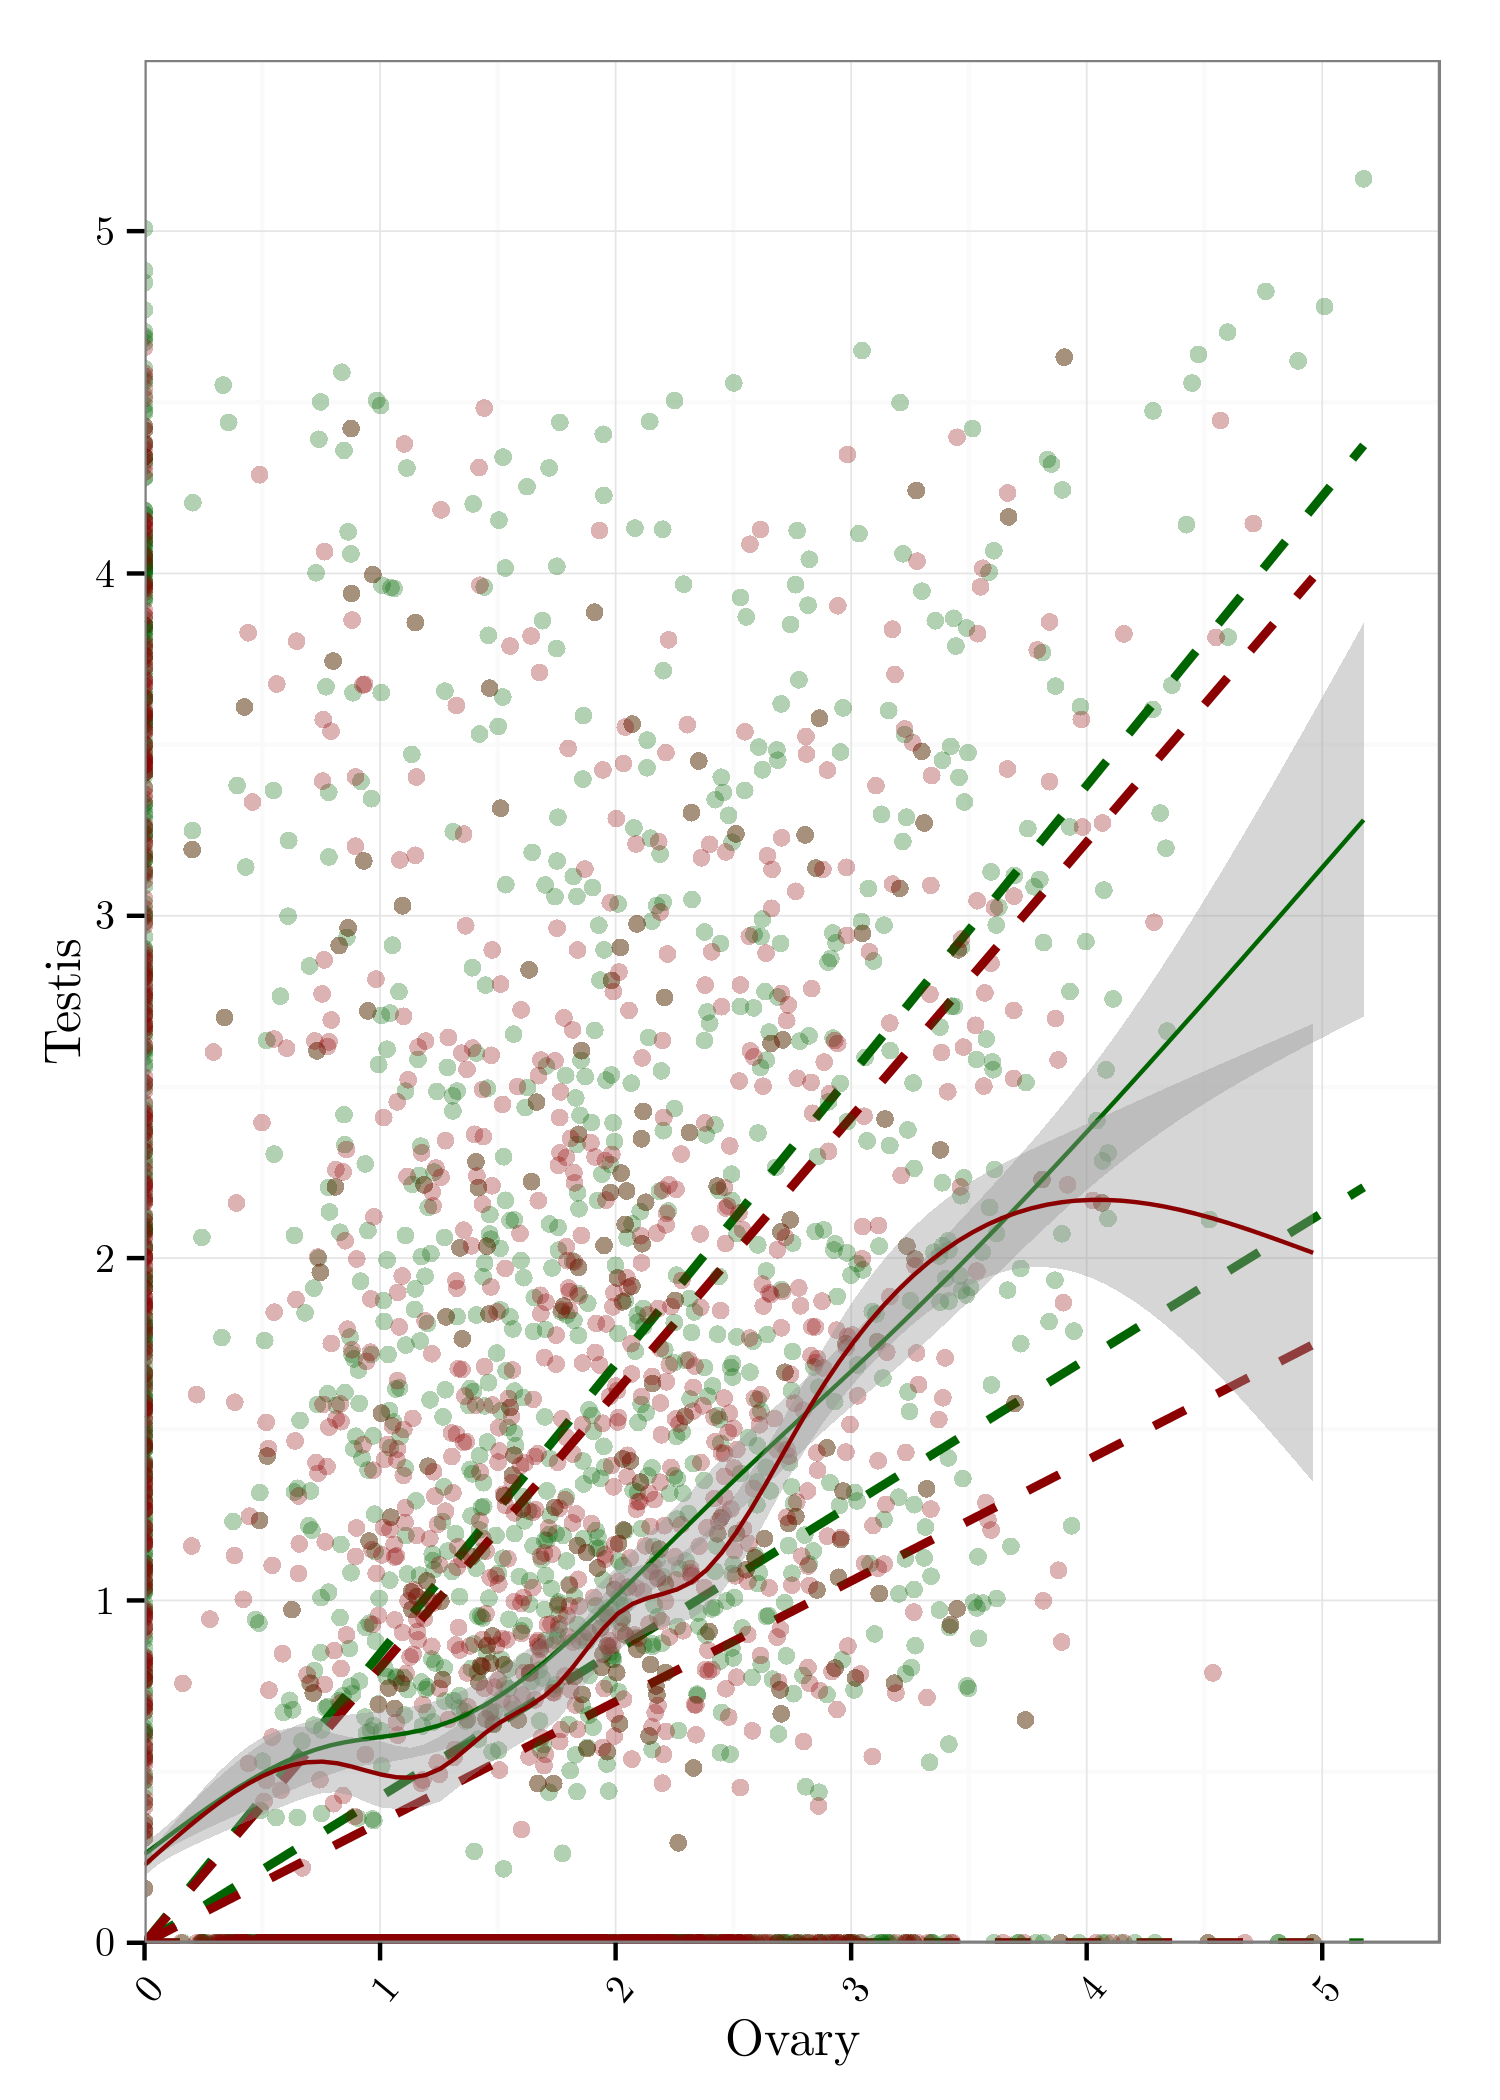
\includegraphics[width=1\linewidth]{pngs/E2F_specific_Male_expression.png}
				\caption{D6 Male developmental stage (Testis).}
			\end{subfigure}
			\caption[Expression values of all genes and genes exclusively targeted by one E2F TF in ovary and testis tissue]
			{Expression values of genes in ovary and testis tissue of animals in the D6 developmental stage.
			(a) All genes;
			(b, c) Genes exclusively targeted by one E2F TF in (b) ovary; (c) testis;			
			Green: E2F1-bound genes;
			Red: E2F7-bound genes;
				{\footnotesize
				Expression values were normalized by the mean expression of all genes within each stage and transformed with a logarithm of base 2;
				Dashed lines indicate quantiles of the distribution of expression values;
				Smoothed line represents the smoothed conditional mean of expression values.
				}
			}
			\label{fig:E2F_targets_expression}
		\end{figure}
		
		\subsubsection{E2F regulation of key cell cycle effectors}
		Since differential regulation of the canonical cell cycle and endocycles arise by the alternative regulation of key cell cycle effectors of progression through the cycles, it is foreseeable that some might be differentially regulated by the E2F TFs in the two gonadal tissues. The vast majority of such key cell cycle regulators components were detected to be putatively regulated by at least one E2F TF in at least one of the tissues. Such effectors are Cyclin, CDK proteins and CKI proteins as well as proteins directly involved in E2F regulation and other known regulators of cell cycle progression such as the co-transcriptional factor DP, the Retinoblastoma protein (Rb), Geminin, Cdt1, Cdh1 and PCNAs. Interestingly all four PCNA genes existent in \textit{Oikopleura} are bound by both TFs in both tissues.
		
		However, due to the lack of replication and the wideness of ChIP-ERs provided by the microarray technology, analysis of discrete cases of gene regulation by E2F factors should be taken with caution. Lists of key cell cycle effectors regulated by E2F TFs can be found in the appendix section \ref{list_key_cell_cycle_regulators}).


\clearpage
\section{Dot1 and H3K79 methylation in \textit{Oikopleura dioica}'s cell cycle modes}
	Methylation of lysine 79 in histone H3 (H3K79me) has been recently shown to be layed in a distributive manner by the Dot1 methyltransferase leading to its accumulation during a cell's cycle \cite{Frederiks2008}. This lead to the proposal H3K79me levels might act as memory for the age of the cell and contribute to the regulation of cell cycle progression \cite{DeVos2011}. Studies on H3K79me and the function of Dot1 in Human cells have shown that knock-out of Dot1 produces cells with a high degree of ploidy due to re-replication in the same cell cycle \cite{Fu2013a}, a situation similar but inverse to \textit{Trypanossoma brucei}, where overexpression of Dot1 has the aforementioned effect \cite{Gassen2012}.
	
	To investigate whether H3K79me would have a function in the regulation of \textit{Oikopleura dioica}'s cell cycle modes and contribute to the differences between them, we conducted an initial functional study on Dot1 through the use of a chemical inhibitor in the Tailbud stage (mitotic) and the Day 5 (endocycle) and characterization of the phenotypic effects.
	
	The Dot1 methyltransferase is ubiquitously expressed throughout the development of \textit{Oikopleura} with no exception (Figure \ref{fig:Dot1_Bre1_expression}a), indicative of its vital function. Nevertheless, the Bre1 ubiquitin ligase, responsible for laying monoubiquitinilation of lysine 123 on histone H2B (H2BK123ub1), of which Dot1 depends to lay its mark, is mostly expressed from the Tailshift developmental stage on (Figure \ref{fig:Dot1_Bre1_expression}a), coincident with the employment of endocycles in \textit{Oikopleura}. In the last day of the life cycle (D6), where sexual dimorphism is most apparent, Bre1 ceases to be expressed in the somatic tissues of the Trunk and in the gonads of female animals, while having the highest expression level of the whole cycle in the male testis, indicating a sex-specific differential use of Bre1 during gonad maturation.
	
	\begin{figure}[h!]
		\setlength{\belowcaptionskip}{5pt}
		\centering
		\begin{subfigure}{1\textwidth}
			\centering
			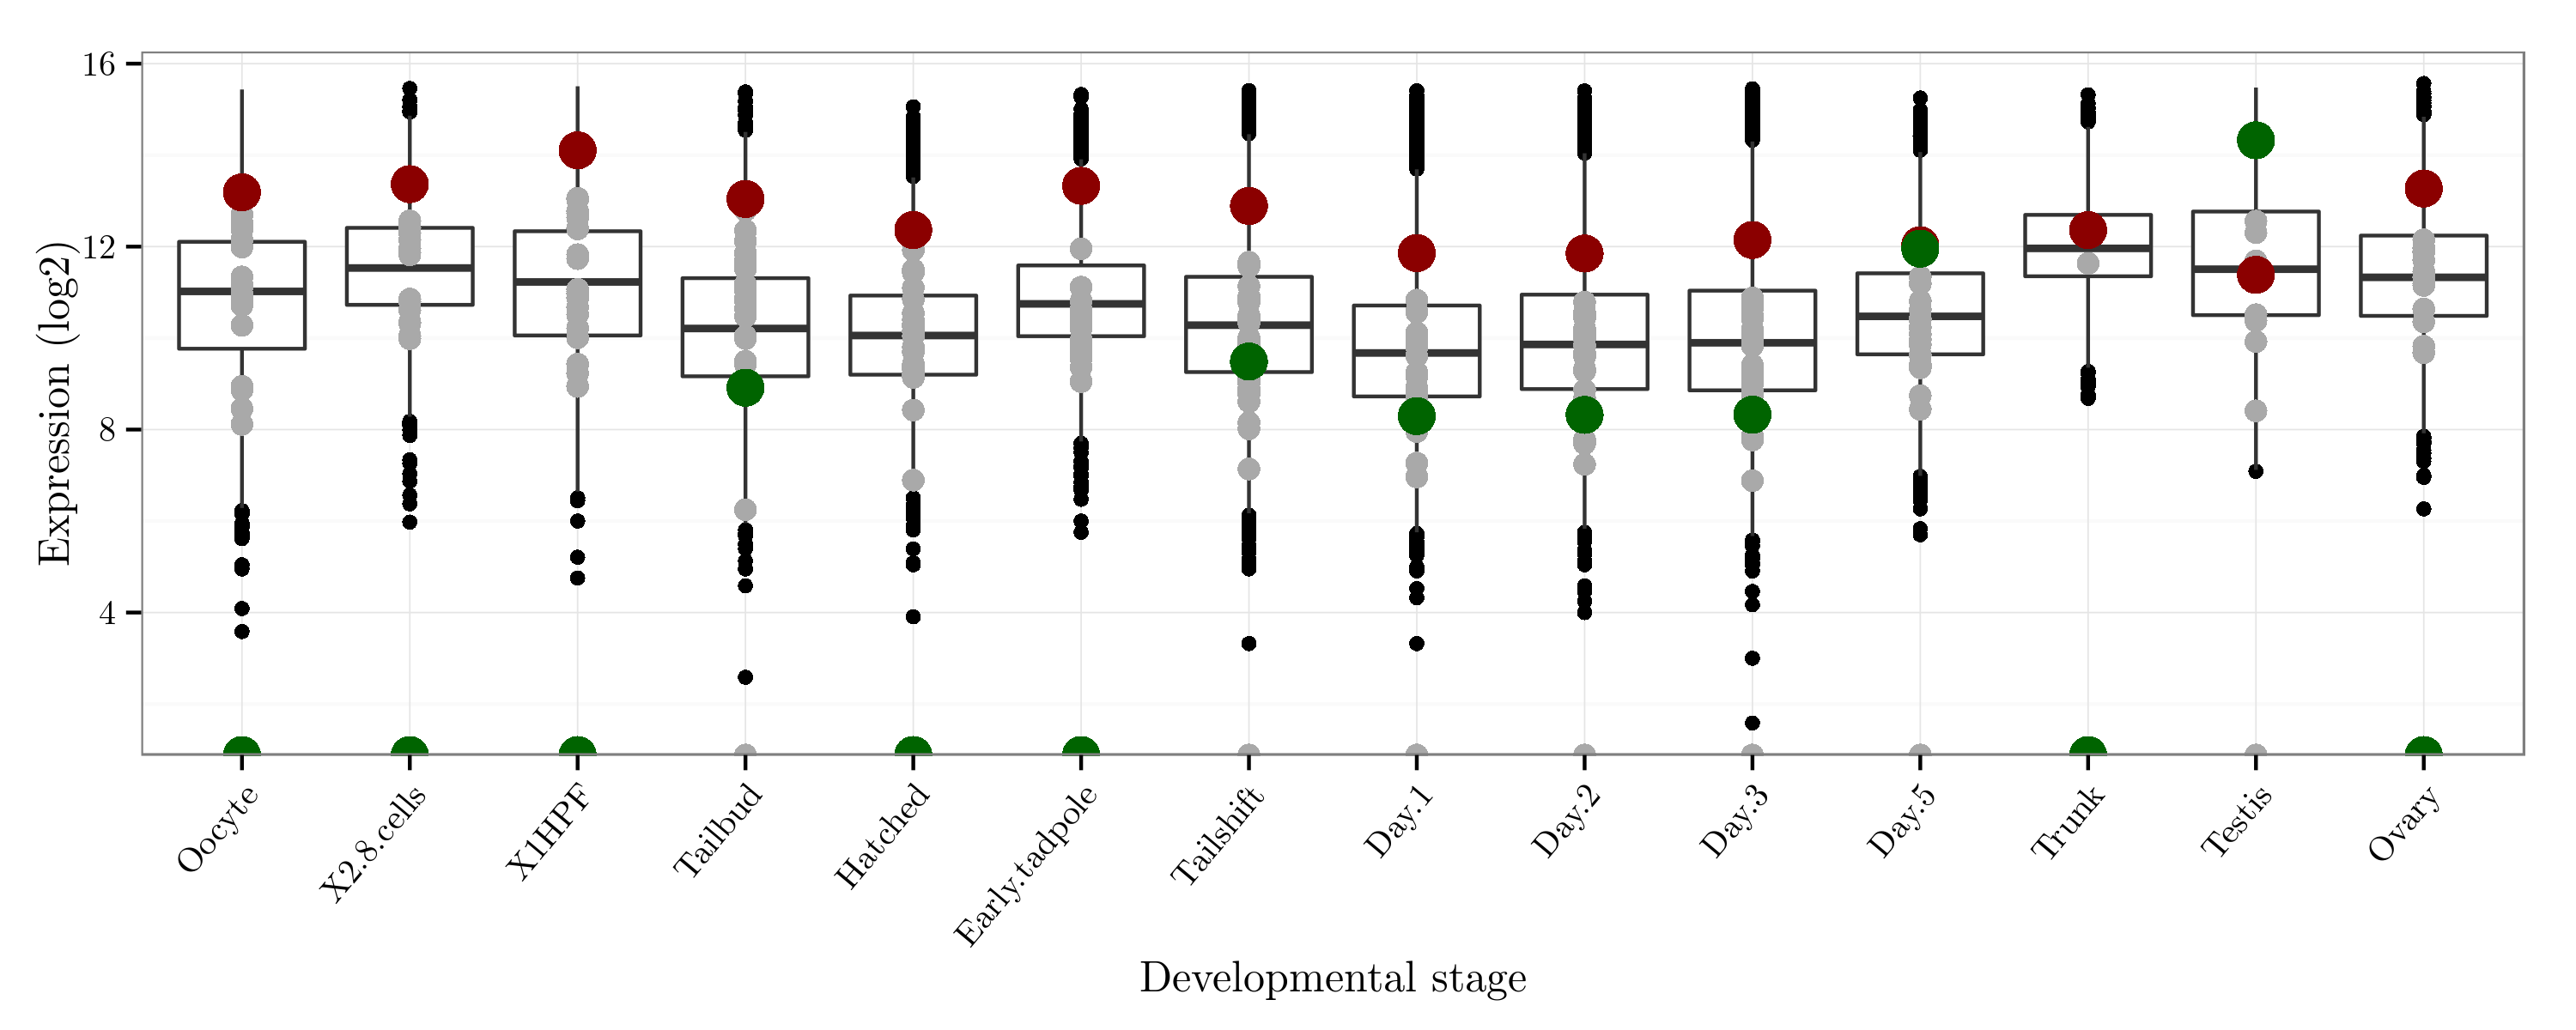
\includegraphics[width=1\textwidth]{pngs/Dot1_expression_allgenes_SETs.png}
			\caption{Life cycle with optimal conditions.}
		\end{subfigure}	
		\begin{subfigure}{.5\textwidth}
			\centering
			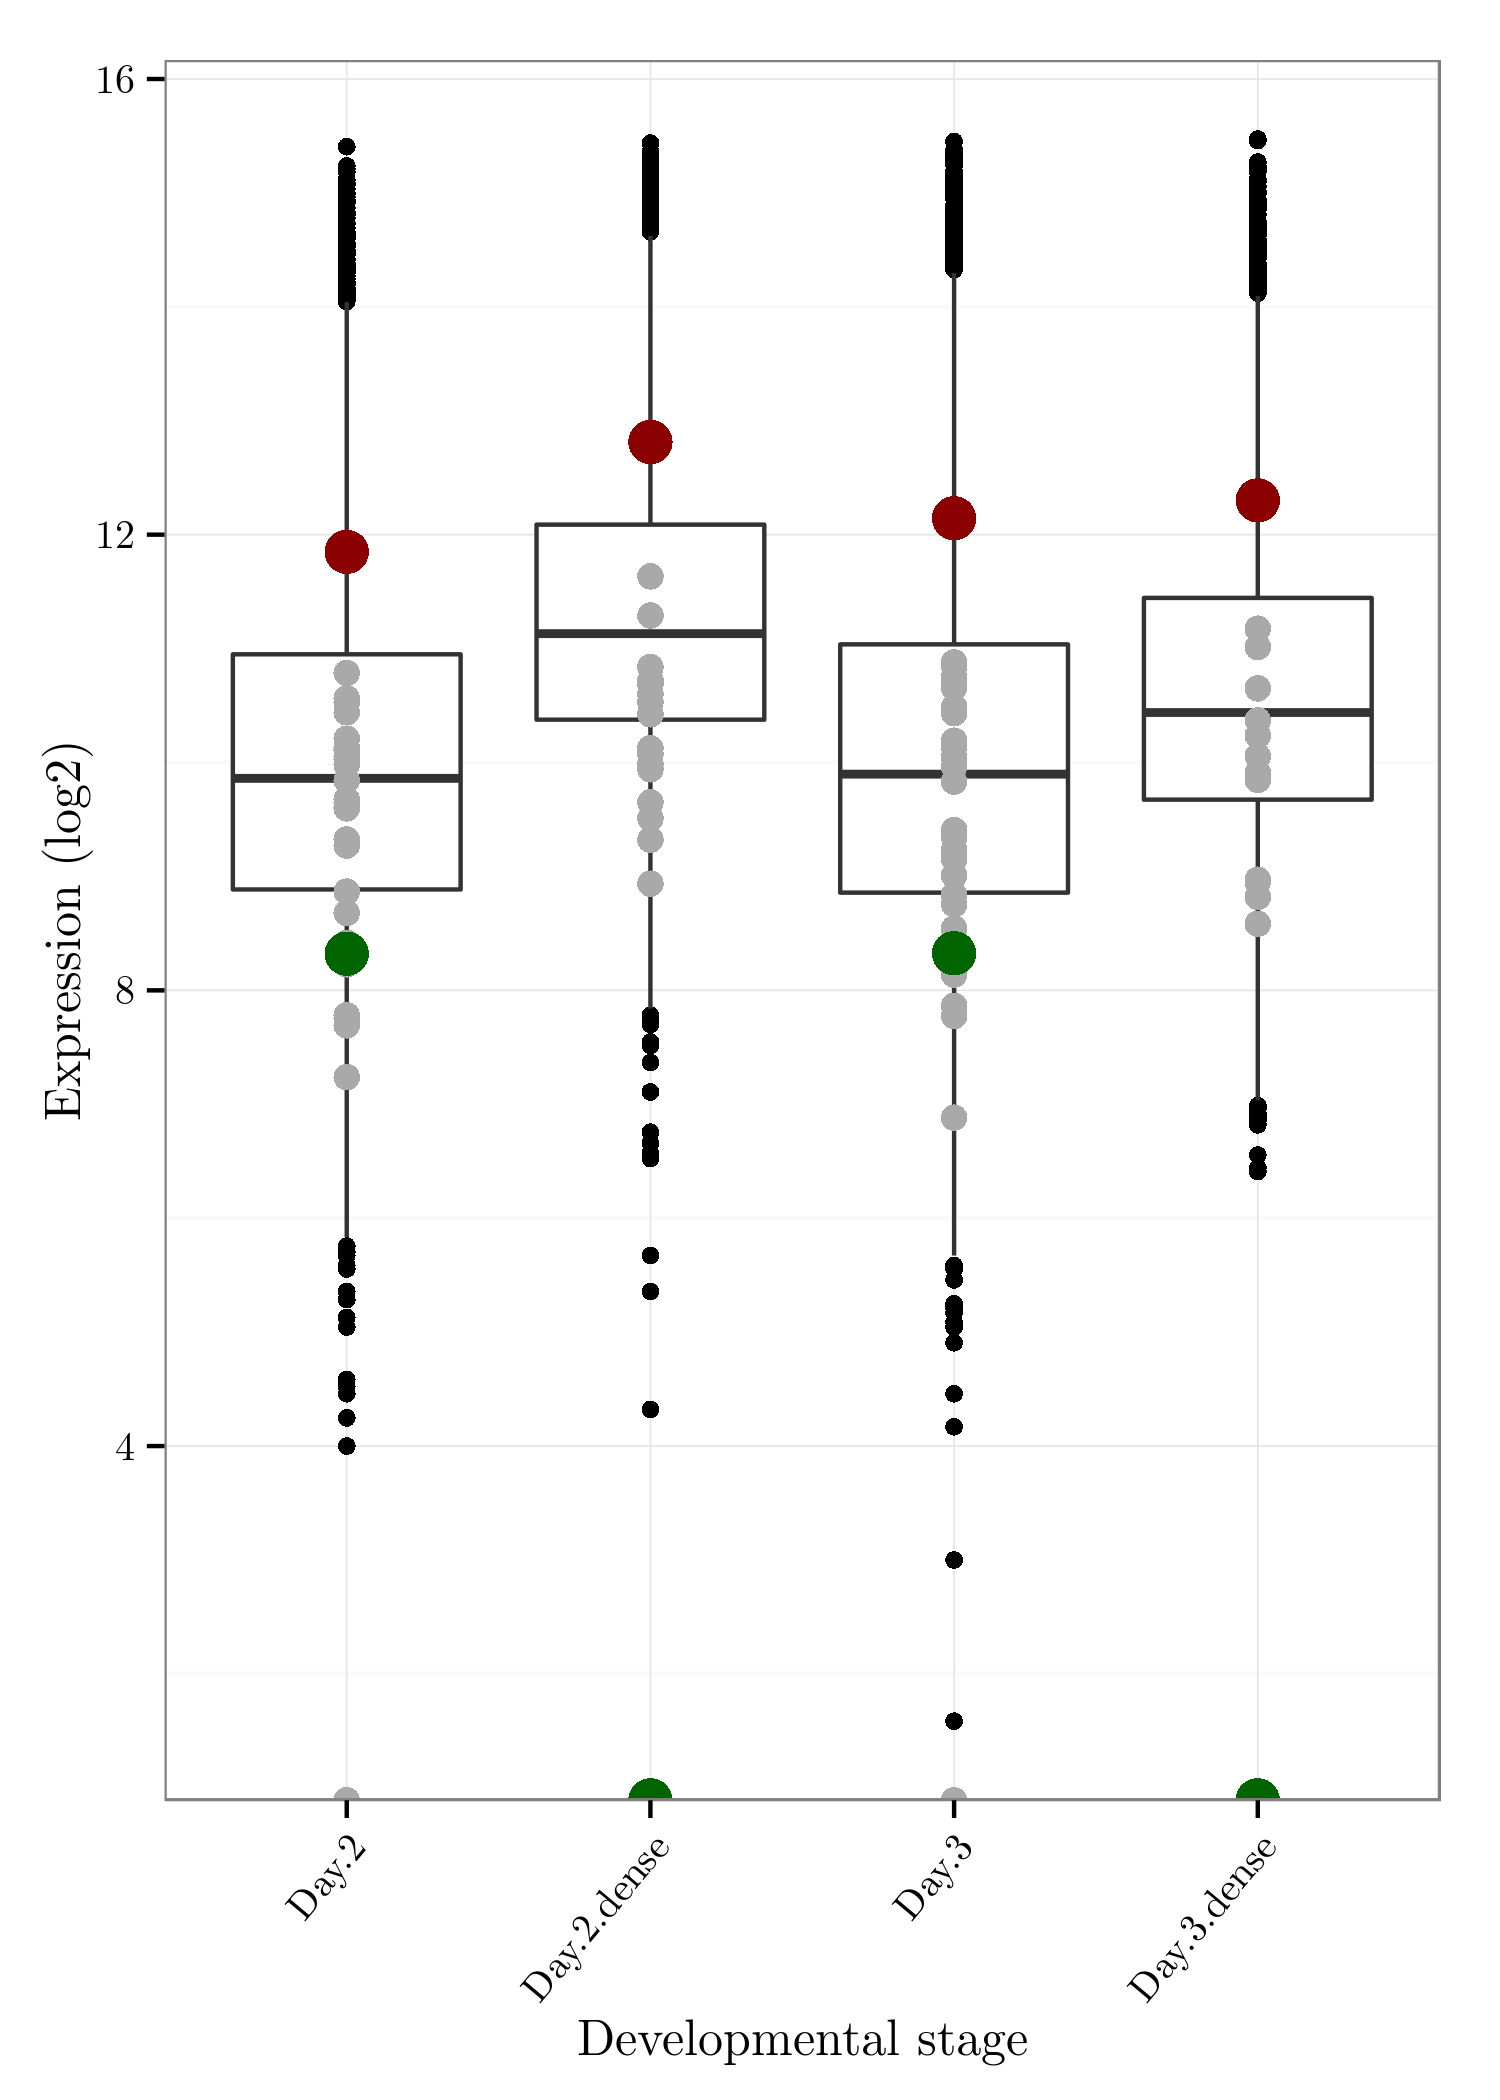
\includegraphics[width=1\linewidth]{pngs/Dot1_expression_allgenes_SETs_dense_noDay4.png}
			\caption{Normal culture and growth arrest (dense) conditions.}
		\end{subfigure}%
		\begin{subfigure}{.5\textwidth}
			\centering
			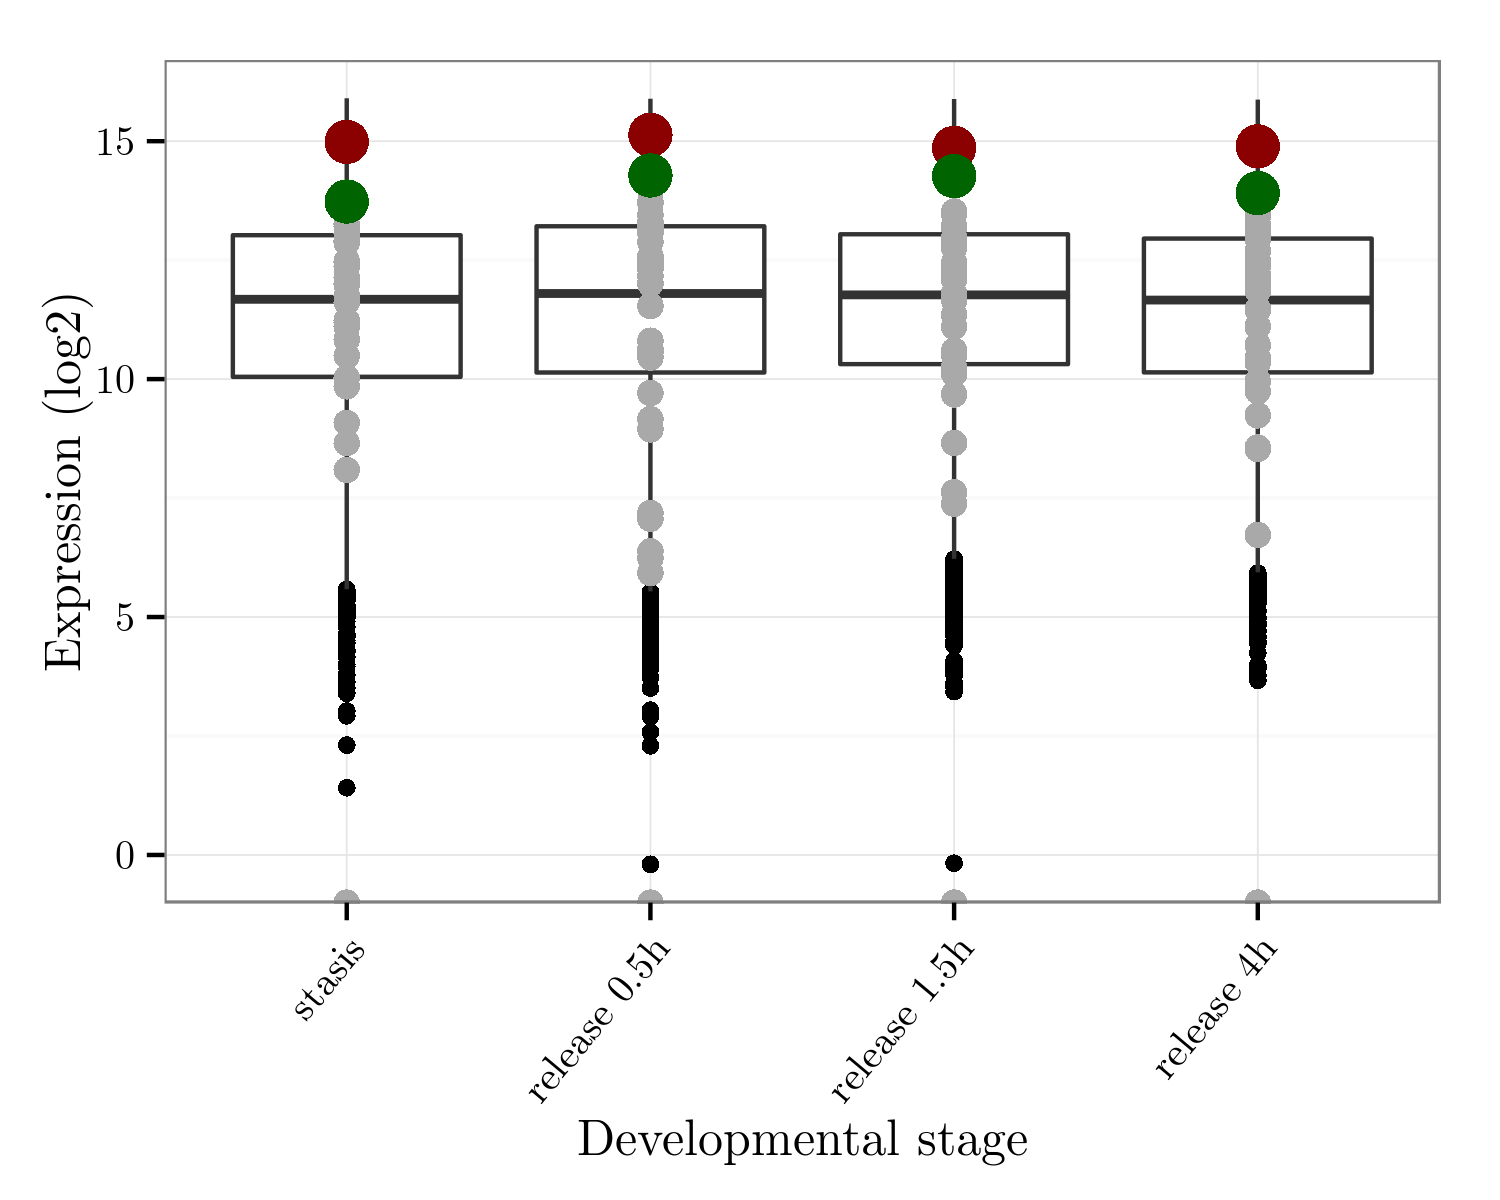
\includegraphics[width=1\linewidth]{pngs/stasisRelease_Dot1_expression_allgenes_SETs.png}
			\caption{After release of growth arrest condition.}
		\end{subfigure}		
		\caption[Expression values of Dot1 and Bre1 enzymes during optimal \textit{Oikopleura} development]
		{Expression values of Dot1 (red), Bre1 (green), all SET domain-containing enzymes (grey) and all genes (boxplots) during (A) optimal \textit{Oikopleura} development. Comparison of (B) normal development and growth arrest, and (C) after release from the growth arrest condition.
		{\footnotesize
			Expression values were transformed with a logarithm of base 2.
			}
		}		
		\label{fig:Dot1_Bre1_expression}
	\end{figure}
	
	\textit{Oikopleura} is known to possess a developmental condition known as growth arrest (GA) with reduced proliferation and growth when cultured densely due to reduced nutritional resources (see section \ref{subsection:Growth_arrest}). During GA, expression of Bre1 is significantly reduced whereas the Dot1 methyltransferase is relatively stable (Figure \ref{fig:Dot1_Bre1_GA_expression}b). When animals are released from the growth arrest condition by restoring the normal culture density and nutritional supply, Bre1 expression is restored to levels compared with normal development during endocycling stages (Figure \ref{fig:Dot1_Bre1_expression}c). This suggests that Bre1 is more highly expressed during periods of proliferation and reinforces the idea it might have a function during endocycles, for this type of cell cycle mode is rapidly inactivated when in GA and resumed when animals are released from this condition \cite{Subramaniam2014}. Nevertheless, this putative increase of activity of Bre1 in endocycles does not imply any particular connection with the increase of H3K79me levels.
	
	To gain more knowledge on the dynamics of H3K79me during \textit{Oikopleura}'s life cycle we assessed the different states of H3K79me by western blot on whole animals (Figure \ref{fig:k79me}a). Developmental stages with a predominant use of endocycles show overall high levels of K79 methylation, while stages with a predominant use of a mitotic cell cycle show decreased levels of K79 methylation. Additionally, in the Tailbud stage (mitotic), the ratio of H3K79me1 to H3K79me3 is in favor of the least methylated form, while on Day 5 all three forms seem equally present and in Day 6 female animals the most methylated form becomes more predominant. In Day 6 male animals, H3K79me3 was atypically detected, probably due to the existence of testis-specific variant of H3, H3.t, which lacks the lysine 79 residue. This suggest that higher methylation forms of H3K79 tend to be more present towards the end of the life cycle of \textit{Oikopleura}, concurrent with the idea of accumulation of H3K79me with time.
	
	\begin{figure}[h!]
		\setlength{\belowcaptionskip}{5pt}
		\centering
		\begin{subfigure}{.5\textwidth}
			\centering
			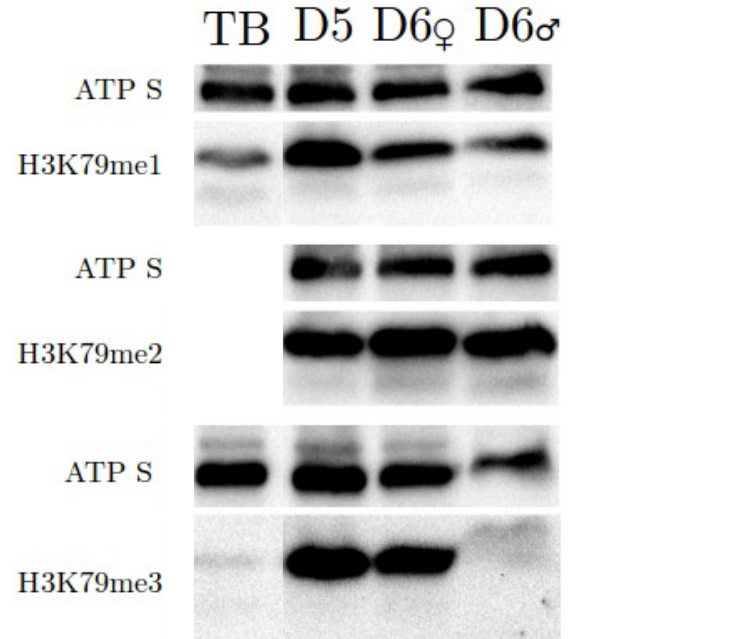
\includegraphics[width=1\linewidth]{pngs/K79me_WT.png}
			\caption{H3K79me in selected developmental stages representative of the different cell cycle modes.}
		\end{subfigure}%
		\begin{subfigure}{.5\textwidth}
			\centering
			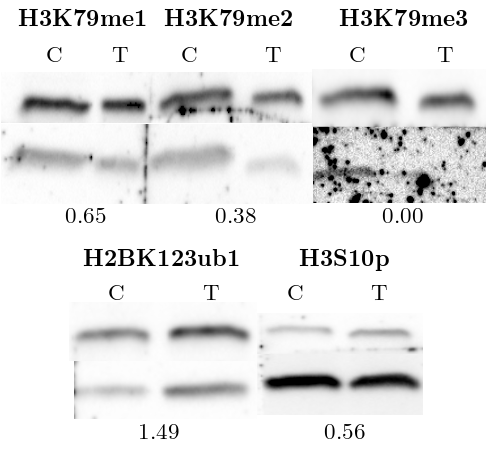
\includegraphics[width=1\linewidth]{pngs/TB_Dot1_in.png}
			\caption{Tailbud stage.}
		\end{subfigure}
		\begin{subfigure}{.7\textwidth}
			\centering
			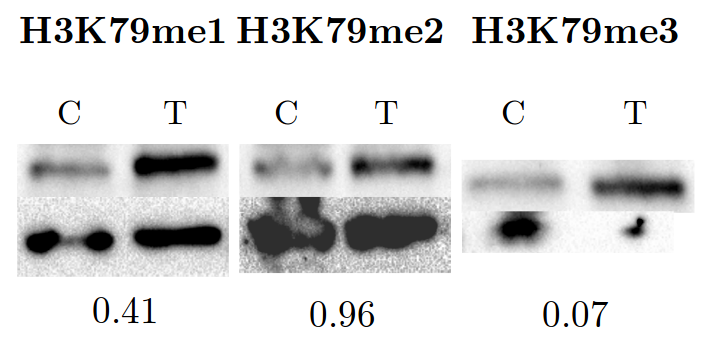
\includegraphics[width=1\linewidth]{pngs/D5_Dot1_in.png}
			\caption{D5 stage.}
		\end{subfigure}
		\caption[H3K79 methylation states during selected developmental stages of \textit{Oikopleura} and in Dot1\textsuperscript{in}-treated animals]
		{Quantification of H3K79 methylation states during selected developmental stages of \textit{Oikopleura dioica}'s life cycle and in Dot1\textsuperscript{in}-treated animals by Western blot.
			{\footnotesize
				In (b) and (c), values under blots show the relative amounts compared with control normalized by ATP synthase $beta$ subunit (upper band). C - DMSO-treated control animals; T - Dot1\textsuperscript{in}-treated animals.
			}
		}
		\label{fig:k79me}
	\end{figure}
	
	To gain knowledge of the function of H3K79me we used a potent and specific chemical inhibitor of Dot1, SGC0946 (from now on Dot1\textsuperscript{in}) \cite{Yu2012} on animals of the Tailbud stage. Treatment with 30 $\mu$M of Dot1\textsuperscript{in} for 3.5 hours was shown to be effective in inhibiting Dot1, as assessed by the reduced levels of H3K79me compared with control animals (treated with the solvent DMSO) (Figure \ref{fig:k79me}b). Depletion of H3K79me was most successful in higher methylation states probably due to the reduced activity of Dot1 on newly deposited histones during replication, since the lower methylation states are necessary for the addition of higher.
	
	Since the presence of H2BK123ub1 is known to increase the deposition of H3K79me by Dot1, we decided to explore the connection between H3K79me and H2BK123ub1, by assessing H2BK123ub1 levels in Tailbud animals treated with Dot1\textsuperscript{in}. Levels of H2BK123ub1 were higher in Dot1\textsuperscript{in}-treated animals when compared with control (treated with the solvent DMSO) (Figure \ref{fig:k79me}b). Although the inverse relationship (dependency of H3K79me on H2BK123ub1) had already been described, increase of H2BK123ub1 in response to decreased levels of Dot1 and H3K79me had not and was therefore surprising. A possible mechanistic explanation could be inspired by the fact that high levels of H3K79me3 were found on the locus of the Bre1 enzyme in testis of animals in D6 developmental stage (P. Navratilova, G. Danks and E. Thompson, unpublished data), a stage where Bre1 expression is notably low (Figure \ref{fig:Dot1_Bre1_expression}a). In this situation, increased H3K79me levels in the Bre1 locus could be responsible for its very low expression, which in turn would reduce the activity of Dot1 creating a negative feedback loop. If this mechanism would be present throughout \textit{Oikopleura}'s life cycle, in the present situation of Dot1 inhibition in the Tailbud stage, H3K79me levels are decreased and Bre1 expression would be enhanced, thus being responsible for the upregulation of the H2BK123ub1 mark in Dot1\textsuperscript{in}-treated animals.
	
	Tailbud animals treated with Dot1\textsuperscript{in} presented phenotypic effects that revealed developmental defects: the surface of the trunk was largely affected, with cells presenting a granulous appearance (Figure \ref{fig:Dot1in_TB}a), failure to maintain swimming activity and later death. To further characterize the phenotype, we assessed the state of cell proliferation by the use of the mitosis marker phosphorilation of serine 10 in histone H3 (H3S10p) and apoptosis by the Tunel assay. The Tunel assay in normal animals revealed cells marked for apoptosis along the tail of animals, starting from the posterior tip and progressing to anteriorly with developmental time (Figure \ref{fig:Dot1in_TB}b), indicating a possible use of apoptosis in regulation of morphogenic processes during this stage of development of \textit{Oikopleura}. Dot1\textsuperscript{in}-treated animals showed reduced levels of H3S10p, indicative of reduced cell proliferation (Figure \ref{fig:k79me}b) signs of apoptosis in the granulous cells of the trunk, specially at its surface (Figure \ref{fig:Dot1in_TB}c).
	
	\begin{figure}
		\setlength{\belowcaptionskip}{5pt}
		\centering
		\begin{subfigure}{1\textwidth}
			\centering
			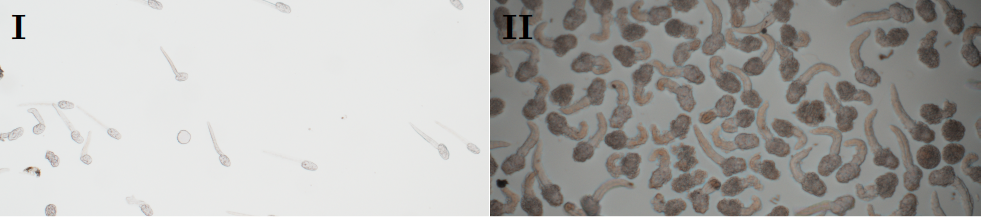
\includegraphics[width=1\linewidth]{pngs/tb_phenotype.png}
			\caption{Phenotypic effects of Dot1in-treated animals compared with DMSO-treated.
				{\footnotesize
					I: DMSO treated;
					II: Dot1in-treated.
					Animals cultured at same densities.
				}
			}
		\end{subfigure}
		\begin{subfigure}{1\textwidth}
			\centering
			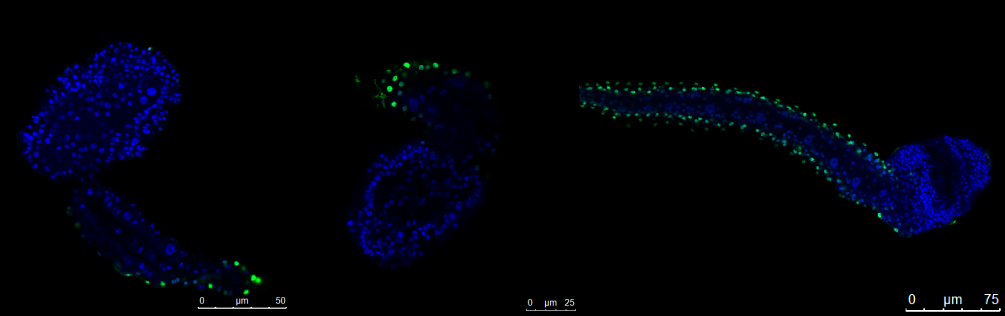
\includegraphics[width=1\linewidth]{pngs/tb_tunnel.png}
			\caption{Tunnel assay on untreated control animals during development of the tadpole.}
		\end{subfigure}
		\begin{subfigure}{1\textwidth}
			\centering
			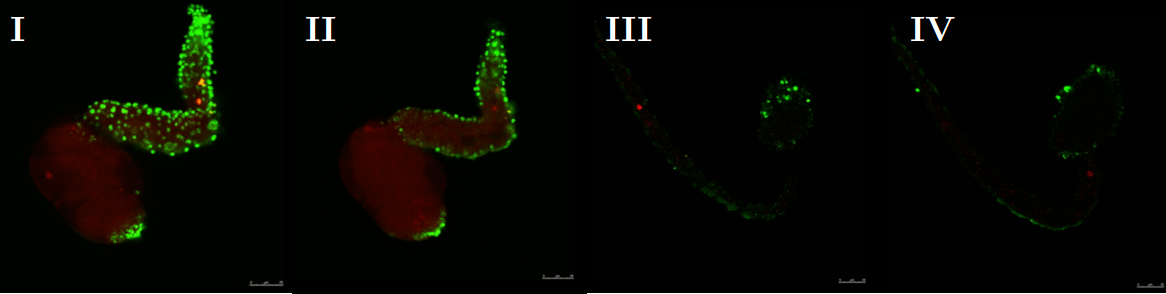
\includegraphics[width=1\linewidth]{pngs/tb_dot1in.png}
			\caption{
				Detection of apoptotic cells using the tunnel assay.
				{\footnotesize
					I-II: DMSO treated;
					III-IV: Dot1\textsuperscript{in}-treated.
				}
			}
		\end{subfigure}
		\caption[Effects of the treatment with Dot1\textsuperscript{in} in Tadpole animals]
		{Effects of the treatment with Dot1\textsuperscript{in} in Tadpole animals. Green: Tunel assay; Red: H3S10p; Blue: DNA;}
		\label{fig:Dot1in_TB}
	\end{figure}
	
	Inhibition of the Dot1 methyltransferase seems to have a severe effect, causing deficiency of proliferation, developmental defects and death in the Tadpole developmental stage of \textit{Oikopleura}, a stage where a mitotic cell cycle is employed. Since Dot1 has been shown to be involved in other developmental processes that may or may not be related with the addition of H3K79me marks (\textit{e.g.} transcription), it is not safe to assume that the phenotypic effects seen are the consequence of H3K79me depletion.
	
	Since the overall amount of H3K79me levels is higher in the endocycling mode of proliferation and the ratio of the methylation states appears to change during the different cell cycle modes, we studied the effects of Dot1 inhibition in the D5 developmental stage, where endocycling is employed extensively in both somatic and gonadal tissues.
	
	Overall levels of H3K79me were reduced although not as much as in the Tailbud stage (Figure \ref{fig:k79me}c). This might be due to the fact that although H3K79me is not copied into new histones during replication, old histones will still carry the same methylation state of H3K79 and because on the D5 stage overall levels of H3K79me are high. This is furthermore amplified by the fact that in the female gonad most nuclei (either nurse or selected oocytes) in the coenocyst are already present at this time, making the most important step of H3K79me dilution - replication - more infrequent. Increased H2BK123ub1 was also detected on Dot1\textsuperscript{in}-treated when compared with control, reinforcing the hipotesis of a indirect negative feedback loop between H3K79me and H2BK123ub1 in \textit{Oikopleura}.
	
	To assess the rate of proliferation of cells in this developmental stage, we measured the incorporation of a labeled nucleotide analog 5-ethynyl-2-deoxyuridine (EdU) using 1 hour pulses and quantifying fluorescence of the labeled nucleotides. In this developmental stage, under optimal conditions cells proliferate actively throughout the \textit{Oikopleura} body, but towards the end of the life cycle (entering Day 6), proliferation is restricted to the gonadal tissue, when somatic tissue ceases to proliferate (Figure \ref{fig:Dot1in_D5}a). In Dot1\textsuperscript{in}-treated D5 animals, gonad proliferation is severely reduced although still detectable (Figure \ref{fig:Dot1in_D5}b) and proliferating somatic cells were detected as opposed to control animals which terminated somatic proliferation as measured by EdU incorporation. Somatic cells marked with EdU were abnormally large and had propensity to detach from the animal body (Figure \ref{fig:Dot1in_D5}c). Surprisingly, animals exhibiting this phenotype remained alive and capable of filtration functions before dying, much later than in the Tailbud stage when comparing time after treatment.
	
	The surprising invertion of the proliferation pattern in the body of 	Dot1\textsuperscript{in}-treated D5 animals might be connected with the function of Dot1 in providing a molecular clock for the cell's age by laying H3K79me and indicate a function for Dot1 in the regulation of proliferation, perhaps by regulating the timing of replication.
	
	\begin{figure}
		\setlength{\belowcaptionskip}{5pt}
		\centering
		\begin{subfigure}{1\textwidth}
			\centering
			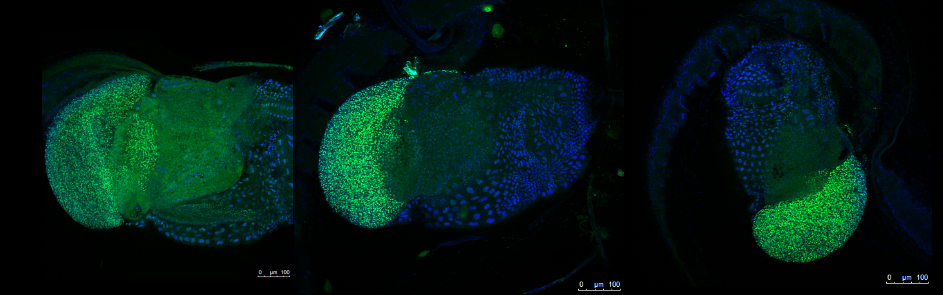
\includegraphics[width=1\linewidth]{pngs/d5_EdU.png}
			\caption{Changes in proliferation during the D5 stage in normal untreated animals.}
		\end{subfigure}
		\begin{subfigure}{1\textwidth}
			\centering
			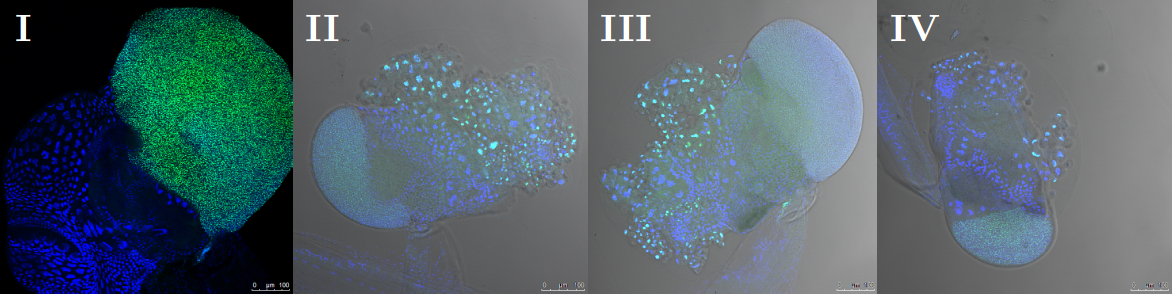
\includegraphics[width=1\linewidth]{pngs/D5_EdU_dot1in.png}
			\caption{
				Changes in proliferation in Dot1in-treated animals compared with DMSO-treated.
				{\footnotesize
					I: DMSO treated;
					II-IV: Dot1in-treated - images overlaid with light microscopy for better detection of the cell's shape.
				}
			}
		\end{subfigure}
		\begin{subfigure}{0.8\textwidth}
			\centering
			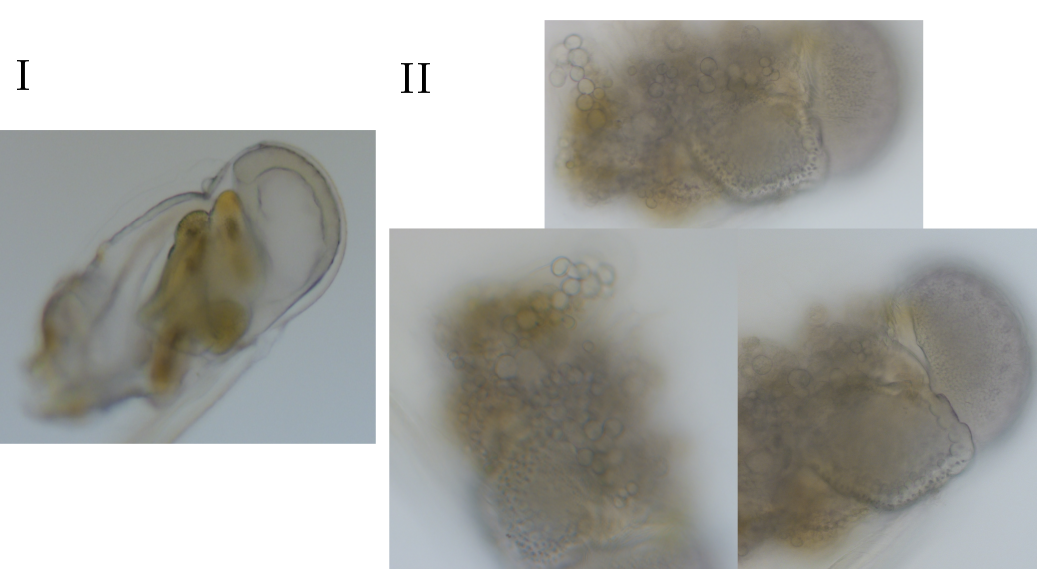
\includegraphics[width=1\linewidth]{pngs/d5_phenotype.png}
			\caption{
				Phenotypic effects of Dot1in-treated animals compared with DMSO-treated.
				{\footnotesize
					I: DMSO treated;
					II: Dot1in-treated.
				}
			}
		\end{subfigure}
		\caption{Assessment of the proliferative state of animals during a predominant endocycle mode of by detection of EdU incorporation.
		Green: EdU;
		Blue: DNA;
		}
		\label{fig:Dot1in_D5}
	\end{figure}

\clearpage

%=========================================================================%
\chapter{Discussion}
%=========================================================================%

\section{E2F factors in \textit{Oikopleura}'s late developmental stages}


\section{Dot1 and H3K79 methylation in \textit{Oikopleura dioica}'s cell cycle modes}

Higher states of K79 methylation accumulate with cell age \cite{DeVos2011}. What are the implications of this in an chordate with a extremely short cell cycle and fast cell division as \textit{Oikopleura}?

Dot1 is more expressed when cultured densely, which might indicate that 
Interestingly, the stage with least Dot1 expression is the testis, where the H3.t H3 variant is more expressed and the K79 residue is not present.

Bre1, the ubiquitin ligase of H2BK123 in yeast and mammals is present in \textit{Oikopleura}, but its expression is not ubiquitous unlike Dot1L. Bre1 is expressed in early stages, although not present maternally (detected earliest in tailbud animals) until day 3. It is not expressed in Day 4, but it is again in Day 5 and has its highest point of expression in the male testis. It is not expressed in the female gonad.

From MS data, H3K79me1/2 were detected, but not me3. me1 is much higher (is the most abundant of all histone PTMs) than me2 \cite{Moosmann2011}, possibly indicating that the state of H3K79me is one of "young cells", marked by low overall levels of H3K79me.


All H3K79me states reduced;
Increased H2Bub (feedback mechanism);
Reduced H3S10p – reduced proliferation;
Apoptosis and death;
H3K79me and Dot1 regulation seem to play a role in the
regulation of Oikopleura's cell cycle modes;
However, validation and more thorough assessment must be
conducted to better elucidate its exact role.
Future studies: dsRNA, overexpression

\clearpage

%=========================================================================%
\chapter{Conclusions and Future Perspectives}
%=========================================================================%




replicates and ChIP-seq data -> more resolution -> more confidence 
Confirmation with ChIP-qPCR
Functional characterization of identified E2F binding sites 
\textit{in vivo} reporter constructs through transgenesis is not yet possible
alternatively,
injections in closely related (or not) species (e.g. Ciona intestinalis)
\textit{in vitro} assays of reporter with luciferase.


Both transcriptional regulation and histone modifications contribute to the regulation of Oikopleura's cell cycle modes;
Analysis of E2F binding in more stages with replication and validation will highlight the differences between mitotic cell cycles and endocycles.


dsRNA knockout
overexpression

Possible role of Dot1 and K79 methylation in the regulation of biological processes known to involve deregulation of replication. Cancer




Regulation at both transcriptional and epigenetic levels is required and probably both play a role in the regulation and transition between \textit{Oikopleura}'s cell cycle modes.



\cleardoublepage
%=========================================================================%
%
% The bibliography
%
%=========================================================================%
\bibliographystyle{plain}
\bibliography{/data/Documents/library.bib}


\cleardoublepage
%=========================================================================%
% Appendix
%=========================================================================%
\begin{appendices}
	\chapter{Gene Ontology terms associated with genes putatively regulated by E2F factors}
	\label{appendix:GOterms}
	
	\chapter{List of key cell cycle regulators putatively regulated by E2F factors}	
	\label{list_key_cell_cycle_regulators}

\end{appendices}


\end{document}
